\documentclass[uplatex,dvipdfmx,a4paper,11pt]{jsbook}

\usepackage{docmute}


% 数式
\usepackage{amsmath,amsthm,amssymb}
\usepackage{bm}
% 画像
\usepackage{graphicx}

\usepackage{multirow}
\usepackage{wrapfig}
\usepackage{ascmac}
\usepackage{xcolor}


\usepackage{makeidx}
\makeindex

\graphicspath{{../../Figures//}{../../Figures/Rheology/}}

\usepackage{qrcode}
\setlength\lineskiplimit{0pt}
\setlength\normallineskiplimit{0pt}

\usepackage{qexam}

\usepackage{titlesec}
\titleformat*{\section}{\Large\bfseries}
\titleformat*{\subsection}{\large\bfseries}
\titleformat*{\subsubsection}{\normalsize\bfseries}
\titleformat*{\paragraph}{\normalsize\bfseries}

% ページ設定
% \pagestyle{empty}
% 高さの設定
\setlength{\textheight}{\paperheight}   % ひとまず紙面を本文領域に
\setlength{\topmargin}{-5.4truemm}      % 上の余白を20mm(=1inch-5.4mm)に
\addtolength{\topmargin}{-\headheight}  % 
\addtolength{\topmargin}{-\headsep}     % ヘッダの分だけ本文領域を移動させる
\addtolength{\textheight}{-40truemm}    % 下の余白も20mmに%% 幅の設定
\setlength{\textwidth}{\paperwidth}     % ひとまず紙面を本文領域に
\setlength{\oddsidemargin}{-5.4truemm}  % 左の余白を20mm(=1inch-5.4mm)に
\setlength{\evensidemargin}{-5.4truemm} % 
\addtolength{\textwidth}{-40truemm}     % 右の余白も20mmに
% 図と本文との間
%\abovecaptionskip=-5pt
%\belowcaptionskip=-5pt
%
% 全体の行間調整
% \renewcommand{\baselinestretch}{1.0} 
% 図と表
%\renewcommand{\figurename}{Fig.}
%\renewcommand{\tablename}{Tab.}
%

% \makeatletter 
% \def\section{\@startsection {section}{1}{\z@}{1.5 ex plus 2ex minus -.2ex}{0.5 ex plus .2ex}{\large\bf}}
% \def\subsection{\@startsection{subsection}{2}{\z@}{0.2\Cvs \@plus.5\Cdp \@minus.2\Cdp}{0.1\Cvs \@plus.3\Cdp}{\reset@font\normalsize\bfseries}}
% \makeatother 

\usepackage[dvipdfmx,%
 bookmarks=true,%
 bookmarksnumbered=true,%
 colorlinks=false,%
 setpagesize=false,%
 pdftitle={数式に頼らない直感的理解による材料設計のためのレオロジー⼊⾨},%
 pdfauthor={佐々木裕},%
 pdfsubject={},%
 pdfkeywords={レオロジー; 材料設計; }]{hyperref}
\usepackage{pxjahyper}

\usepackage{plext}

\usepackage{niceframe} 
\usepackage{framed}
\newenvironment{longartdeco}{%
  \def\FrameCommand{\fboxsep=\FrameSep \artdecoframe}%
  \MakeFramed {\FrameRestore}}%
 {\endMakeFramed}
 
\usepackage{siunitx}

\newcommand{\rmd}{\mathrm{d}}

\title{数式に頼らない直感的理解による\\材料設計のためのレオロジー⼊⾨}
\author{佐々木裕}
\date{\today}

\begin{document}

\maketitle

\frontmatter

\chapter*{まえがき}

\section*{レオロジーとは}
我々の身の回りの材料の大半は流れるという性質を持っています。
当然、それぞれの材料ごとに流れ易さは異なりますが、非常に長い時間をかければ不動に見える岩や大地も流れていきます。
その流れるものを測る学問がレオロジーです。

レオロジーは「お触りの科学」とも言われています。
人間の五感(特に触覚)は極めて優秀であり、手触りで物質の特徴の違いを直感的に区別することができます。
しかしながら、この直感的な区別を材料や商品の開発へと結びつけることは困難です。
それは、直感的な区別はあくまでも定性的なものであり、定量性に欠ける場合がほとんどであるためです。

\section*{目指すもの}
レオロジーの本質をきちんと理解することで、各種の材料の違いを明確に区別する方法がイメージでき、その違いを利用した材料の設計のポイントもわかってきます。

直感的に感じる違いをきちんとした理解へと結びつけるために、本セミナーでは、「箇条書き」や「図解」を多用します。
そうすることで、単に抽象的な概念としてだけではなく、ブレイクダウンしたイメージとして直感的に捉えていきます。
また、数式だけに頼ることなく、数式が表したいことを理解して、イメージと数式をつなげていきます。

本セミナーは、レオロジーを実践的に使いこなすためのベースとなる基本的な事項を実感として理解し、材料の持つ「流動と弾性」という二面性をイメージとして持てるようになることを目指します。

\section*{簡単な自己紹介}

筆者は、もともと合成化学をベースとした高分子化学を専攻し、1986 年に化学系材料のメーカーである東亞合成株式会社に入社しました。
入社当初の仕事としては、新規構造を有する材料の合成を主として各種の光硬化型材料の研究開発を行ってきました。
その自身が合成した材料の特性評価を行う過程において、レオロジーを始めとした各種の材料評価技術の習得へとつなげてきています。

これらの経験において、「新規なものを作り出す技術としての化学の有用性」を何度も再認識してきました。
それと同時に、物理、数学、統計等の中にある「事象を客観視しながら普遍性を大事にするものの考え方」の重要性を痛感する場面も幾度となく経験してきました。
そして、それらの場面において最も役立ったのは、レオロジーから学んだマクロな応答をミクロな化学構造へと繋げられる想像力でした。

このような感覚を皆さんにお伝えできればと望んでおります。

\begin{screen}
	\begin{itemize}
		\item 略歴
        \begin{itemize}
            \item 北海道大学で合成化学系の高分子化学を専攻
			\item 卒業後、東亞合成株式会社に入社し、現在に至る
		\end{itemize}
		\item  研究・開発歴
		\begin{itemize}
			\item 合成をベースとした各種の光硬化型材料の研究開発に従事。
			\item 機能性材料の特性評価を通して、レオロジー等の評価技術の重要性を痛感。
			\item 現在は、シミュレーションやレオロジーを主として研究活動を継続。
		\end{itemize}
		\item モットー
		\begin{itemize}
            \item 「化学をベースに、尤もらしく」
			\item 「物理、数学、統計の考えを利用して」
		\end{itemize}
	\end{itemize}
\end{screen}

\section*{本講座の進め方}

本講座においては、実際の研究開発に役に立つレオロジー関連の事項について、基礎的な事項をきちんと押さえながら、直感的に理解していくことを目指して説明を行います。

以下のような点に気を付けて、進めていきたいと考えています。
\begin{boxnote}
	\large
	\begin{itemize}
		\item 進め方のポイント
		\begin{itemize}	
			\item
			  イメージしやすい、直感的な理解を目指す。
			  \begin{itemize}
			  \item
				全体を俯瞰した概念的な説明
			  \item
				多様な切り口からの説明
			  \end{itemize}
			\item
			  大事なことは何度か繰り返す。
			  \begin{itemize}
			  \item
				一度ではわかりにくいかも。
			  \item
				似たような内容を、ちょっと違う言葉で。
			  \end{itemize}
			\item
			  ゆっくり議論
		\end{itemize}
		\item 数式に頼らないという意味
		\begin{itemize}
			\item 状態をイメージするためには、数学的な感覚は有効
				\begin{itemize}
					\item 直感的に感じるイメージを数学とつなげて理解すれば、\\
					共有しやすい。
					\item そのために、数学(算数?)的な事項の復習もやります。
				\end{itemize}
			\item 「天下りの数式展開」は無駄。
				\begin{itemize}
				\item 意味の理解できない数式は無意味。
				\item たいてい、思考停止を招くだけ。
				\item 数式の表す内容をイメージしましょう。
				\end{itemize}
		\end{itemize}
	\end{itemize}
\end{boxnote}

また、本講座では、できるだけ数式には頼らない説明を目指します。

ただ、「数式に頼らない」ということは、「数式を使わない」という意味ではありません。
本論でお話しますように、我々がレオロジーを使いこなして行くためには、対象となる物質の状態をきちんとイメージすることが重要になります。
そのイメージングの際に、数学的な感覚は非常に役に立つものなのです。

私に分かり易い表現があなたにとっても有効とは限らないので、数式の表すものを一緒に考えていきましょう。

\setcounter{tocdepth}{2}
\tableofcontents

\mainmatter

\setcounter{chapter}{0}

\chapter{レオロジーとは}
\documentclass[uplatex,dvipdfmx,a4paper,11pt]{jsreport}

\usepackage{docmute}


% 数式
\usepackage{amsmath,amsthm,amssymb}
\usepackage{bm}
% 画像
\usepackage{graphicx}

\usepackage{multirow}
\usepackage{wrapfig}
\usepackage{ascmac}
\usepackage{xcolor}


\usepackage{makeidx}
\makeindex

\graphicspath{{../../Figures//}{../../Figures/Rheology/}}

\usepackage{qrcode}
\setlength\lineskiplimit{0pt}
\setlength\normallineskiplimit{0pt}

\usepackage{qexam}

\usepackage{titlesec}
\titleformat*{\section}{\Large\bfseries}
\titleformat*{\subsection}{\large\bfseries}
\titleformat*{\subsubsection}{\normalsize\bfseries}
\titleformat*{\paragraph}{\normalsize\bfseries}

% ページ設定
% \pagestyle{empty}
% 高さの設定
\setlength{\textheight}{\paperheight}   % ひとまず紙面を本文領域に
\setlength{\topmargin}{-5.4truemm}      % 上の余白を20mm(=1inch-5.4mm)に
\addtolength{\topmargin}{-\headheight}  % 
\addtolength{\topmargin}{-\headsep}     % ヘッダの分だけ本文領域を移動させる
\addtolength{\textheight}{-40truemm}    % 下の余白も20mmに%% 幅の設定
\setlength{\textwidth}{\paperwidth}     % ひとまず紙面を本文領域に
\setlength{\oddsidemargin}{-5.4truemm}  % 左の余白を20mm(=1inch-5.4mm)に
\setlength{\evensidemargin}{-5.4truemm} % 
\addtolength{\textwidth}{-40truemm}     % 右の余白も20mmに
% 図と本文との間
%\abovecaptionskip=-5pt
%\belowcaptionskip=-5pt
%
% 全体の行間調整
% \renewcommand{\baselinestretch}{1.0} 
% 図と表
%\renewcommand{\figurename}{Fig.}
%\renewcommand{\tablename}{Tab.}
%

% \makeatletter 
% \def\section{\@startsection {section}{1}{\z@}{1.5 ex plus 2ex minus -.2ex}{0.5 ex plus .2ex}{\large\bf}}
% \def\subsection{\@startsection{subsection}{2}{\z@}{0.2\Cvs \@plus.5\Cdp \@minus.2\Cdp}{0.1\Cvs \@plus.3\Cdp}{\reset@font\normalsize\bfseries}}
% \makeatother 

\usepackage[dvipdfmx,%
 bookmarks=true,%
 bookmarksnumbered=true,%
 colorlinks=false,%
 setpagesize=false,%
 pdftitle={数式に頼らない直感的理解による材料設計のためのレオロジー⼊⾨},%
 pdfauthor={佐々木裕},%
 pdfsubject={},%
 pdfkeywords={レオロジー; 材料設計; }]{hyperref}
\usepackage{pxjahyper}

\usepackage{plext}

\usepackage{niceframe} 
\usepackage{framed}
\newenvironment{longartdeco}{%
  \def\FrameCommand{\fboxsep=\FrameSep \artdecoframe}%
  \MakeFramed {\FrameRestore}}%
 {\endMakeFramed}
 
\usepackage{siunitx}

\newcommand{\rmd}{\mathrm{d}}

% \title{第一章 レオロジーとは}
% \author{}
% \date{}

\begin{document}

% \maketitle

% \setcounter{chapter}{1}
\chapter{レオロジーとは}

\section*{この章の内容}

ここでは、レオロジーという「考え方」についての説明から始めていきます。
レオロジーを学ぶことで会社の仕事に活かせるような考え方を身に付けていただきたいと思います。

以下に、この章で議論する内容について簡単にまとめました。

\begin{boxnote}
	\large
	\begin{itemize}
		\item レオロジーとは?\\はじめに、「レオロジー」という言葉について、概観しましょう。
		\begin{itemize}
			\item レオロジーの歴史的背景を振り返り、その流れを確認します。
			\item 具体的なレオロジーのやり方について説明します。
		\end{itemize} 
		\item 会社の仕事とレオロジー\\会社の仕事とレオロジーの関わりについて考えてみます。
		\begin{itemize}
			\item レオロジーが関わる分野が非常に広範囲に渡ることを確認します。
			\item 会社の仕事とレオロジーの関わりについて考えてみます。
			\item 特に商品を作り出すときの有効性について見てみます。
		\end{itemize} 
		\item 人の感覚とレオロジー\\人間の直感とレオロジーとの親和性が高いことについて考えてみます。
		\begin{itemize}
			\item レオロジーは、「おさわりの科学」とも言われています。
			\item 人間の五感が大事であることを再確認します。
			\item そして、人間の判断基準についても説明します。
		\end{itemize}
		\item レオロジーを理解するために\\有用なレオロジーですが、その理解は困難な場合も多く見受けられます。
		\begin{itemize}
			\item レオロジーの理解を妨げる要因について簡単にまとめます。
			\item おすすめの理解へのアプローチについて紹介します。
		\end{itemize} 
	\end{itemize}
\end{boxnote}

\section{レオロジーとは?}

まず、レオロジーという言葉のはじまりを確認し、どのような考え方であるのかを概観していきましょう。

\subsection{レオロジーの始まり}
1929年にアメリカにおいてレオロジー学会 The Society of Rheology (SOR) が設立されました。
このとき、中心となったのが、E.C. Bingham でした。
レオロジーという言葉は彼の造語であり、万物流転という意味を表すギリシア語の ``\textit{panta rhei}'' から引いた接頭語である ``Rheo-'' を学問の分野を表す ``-logy'' と組み合わせたものです。
そして、その対象を「物質の変形と流動に関する科学」と定めたのでした。
\begin{figure}[htb]
	\begin{center}
		\begin{minipage}{0.5\textwidth}
			\large
			\begin{itembox}[l]{レオロジーの始まり}
				レオロジー (Rheology) とは、\\
			「物質の変形と流動に関する科学」
				\begin{itemize}
					\item \textit{panta rhei} (ギリシア語)
					\item ``everything flows''
					\item 万物流転
				\end{itemize}
			\end{itembox}
		\end{minipage}
		\begin{minipage}{0.4\textwidth}
			\begin{center}
				\includegraphics[width=0.6\textwidth]{Bingham.jpg}\\
				\large{\bf Eugene Cook Bingham}
			\end{center}
		\end{minipage}
	\end{center}
		\caption{レオロジーの創始者}
		\label{Bingham}
\end{figure}

日本では、それから約二十年後の 1951 年に第1回レオロジー討論会が開催されています。
学会としてレオロジー学会が設立されたのは、その二十年以上後の 1973 年になります。
ですから、学問と考えれば、それほど歴史が古いわけでもないことになります。
その後、現在に至るまでその発展は続いており、非常に多様な分野へと適応される範囲は広がってきています。

\subsection{レオロジーのやり方}

そもそも、物体の変形や流動に関する物理学は、古くから弾性論\index{だんせいろん@弾性論}や流体論\index{りゅうたいろん@流体論}として存在していました。
弾性論は Hooke の法則\index{ふっくのほうそく@Hooke の法則}を基本にして弾性固体を、そして、流体論はNewton の法則\index{ニュートンの法則@Newton の法則}により粘性を持つ単純な流体を対象として、物体の挙動を明確にしていたのでした
\footnote{
	Hooke の法則、Newton の法則については、後ほどきちんと説明しますので、安心してください。
}。
\begin{figure}[htb]
    \begin{center}
        \includegraphics[width=.9\textwidth]{Rheo_method.png}
        \caption{レオロジーのやりかた}
        \label{yarikata}
    \end{center}
\end{figure}

レオロジーは、弾性固体とか粘性流体のような「理想的な物体」に限ること無く、我々が日々に遭遇する「一般にそこらに存在する物質や材料」を対象に含んでいます。
言い換えれば、対象を問わず、その変形と流動に関する事柄をすべて取り扱うということになり、物理学、化学、生物学、地学、医学、薬学、農学、食品学、家政学、時には心理学までをも含む多くの学問分野に横断的に関係する極めて学際的な学問となっています。

レオロジーは、そもそも科学の一分野として提唱されたわけですが、変形や流動というキーワードで物質や材料の特性を評価できることになりますから、実学として工学的にも大きな意味を持って来ています。
これが、広くレオロジーが用いられるようになった大きな要因となります。

レオロジーを測定する具体的な方法は、物質に外的な刺激を与えて、その応答としての変形や流動を測ることになります。
一般に、その刺激とは物質に力\index{ちから@力}や変形を与えることであり、応答としては時間という因子を意識しながら物質の流動や返してくる力\footnote{
	このあとに詳細を学びますが、このときの返してくる力は「応力\index{おうりょく@応力}」という物質内部での内力と呼ばれるものとなります。
}を測定することになります。
そして、このような測定を通して、物質の持つ各種の特性を比較することができるようになるわけです。

この考え方を簡単に書き直すと、図 \ref{yarikata} に示したようになります。

\section{会社の仕事とレオロジー}

ここでは、レオロジーの関わる分野が多様であることを確認し、その多様性を会社の仕事に生かしていくということについて考えてみましょう。

\subsection{レオロジーの関わる分野}

前述したように、1929年にアメリカにおいて、Bingham を中心としてレオロジー学会 The Society of Rheology (SOR) が設立されました。
日本では、それから約二十年後の 1951 年に第1回レオロジー討論会が開催されています。
その後、多様な分野へとその適応される範囲は広がってきています。

例えば、2019 年に開催された第 67 回レオロジー討論会に協賛した学会を見てみましょう。
\begin{screen}
	日本材料学会、プラスチック成形加工学会、高分子学会、日本化学会、日本物理学会、繊維学会、応用物理学会、化学工学会、
	強化プラスチック協会、日本ゴム協会、日本接着学会、日本セラミックス協会、日本木材学会、セルロース学会、日本機械学会、
	日本雪氷学会、日本混相流学会、日本流体力学会、可視化情報学会、日本食品科学工学会、日本家政学会、日本調理科学会、
	日本食品工学会、日本繊維機械学会
\end{screen}

非常に多様な学会が協賛しており、レオロジーという学問が学際的な特徴を有していることがわかります。

さらに、それぞれの学会が関連している分野を考えると、学術的な分類だけではなくて材料の種類や応用の範囲にしても、以下のように非常に幅広い分野に渡っていることが理解できます。
	\begin{itemize}
	\item
	  学術分野:化学、物理、生物、化学工学、応用物理、流体力学、地球物理学
	\item
	  高分子化学(科学):プラスチック、繊維、ゴム、強化プラスチック
	\item
	  材料:金属、セラミックス、木材
	\item
	  応用:機械、接着、塗料、食品化学、調理科学、家政学、成型加工
	\end{itemize}
	
したがって、レオロジーとは、高度に学際的な科学であると同時に、それぞれの要素技術が大きく異る多岐にわたる対象を、多様な切り口で議論していくことが出来るアプローチとも捉えられます。

\begin{figure}[htb]
	\begin{center}
		\includegraphics[width=.9\textwidth]{Katsuyou.png}
		\caption{レオロジーの活用}
		\label{katsuyou}
	\end{center}
\end{figure}

\subsection{会社の仕事とレオロジー}

次に、会社の仕事とレオロジーの関係について考えてみましょう。
この講座に参加されているみなさんの大多数は、会社に勤務されていると思います。
ここで、会社の社会的な意味について確認しておきましょう。

一般に、会社は営利団体であり、利益を生み出すことでその存在を継続させ、社会的な意義を果たしていくことになります。
そして、製造に関連する会社であれば、商品(製品)を作り出し、製造、販売することで、その利益を生じているわけです。

商品の開発の流れを簡単に言えば、原料から材料、そして商品へと価値を付与できるようにつなげていく過程と考えることができます。
そして、それぞれのステップで評価・解析に基づく、設計を行っていくわけです。
その設計の過程において商品に必要となる特性を評価する際に、レオロジーを活用することが多いわけです。
模式図とすれば、図 \ref{katsuyou} に示したようなイメージとなります。

\subsection{レオロジーと商品}

以前に図示(図 \ref{yarikata})したように、レオロジーとは物質に刺激を与えてその応答を評価観察することで、その特性を評価できるのでした。

では、商品化におけるレオロジー利用の、具体的な例を見てみましょう。
以下に示したように、人間の心地良さの定量化や、原料、材料の機能設計にレオロジーが活用されている事例が多くあります。
\large
	\begin{itembox}[l]{レオロジーが活用されている例}
		\begin{itemize}
			\item
			人間の心地良さの定量化にレオロジー的感覚で評価
			\begin{itemize}
				\item 食品工学における「舌触り」や「のど越し」のような食感の定量化。
				\item 肌触りの良い下着やノビの良い化粧品のような触感の定量化
			\end{itemize}
			\item
			原料、材料の機能設計にレオロジーを利用
			\begin{itemize}
			\item
				ショックのない運動靴やよく飛ばせるゴルフクラブのような力学特性の評価
			\item
				塗り易くて液だれしない塗料のような流動特性の評価
			\end{itemize}
		\end{itemize}
	\end{itembox}
\normalsize
したがって、少なくとも定性的に物事を評価するためには、レオロジーが非常に有効な方法であることが理解できるでしょう。

\section{人の感覚とレオロジー}
\label{sec:1_kankaku}

前節で、人間の心地良さのような感覚を評価するためにレオロジーが使えるという事例を示しました。
このことについて、もう少し詳しく考えてみましょう。

\subsection{人はみなレオロジスト}

\subsubsection{オノマトペとレオロジー}

オノマトペ\index{おのまとぺ@オノマトペ}とは、状態や感情を言葉に表したものであり、この語彙が多彩で豊富であることが日本語の大きな特徴の一つとなっています。
織物などの手触りのような質感を意味する言葉として、テクスチャという言葉もあります。
手触りだけでなく食品分野で食感を表現するためにも、テクスチャを表すオノマトペが多用されています。

レオロジーに、単純につながるような物性を表す言葉としては、「サラサラは低粘度、ドロドロは高粘度」や「ふにゃふにゃは低弾性、カチカチは高弾性」のようなものもありますし、これが、フワッフワとかモッチモチになると、一層感覚的な表現になってきます。
このような感覚は、別に若者言葉として特別なのではなくて、日本人には共通認識として通じる感覚になっています。
\begin{figure}[htb]
	\begin{center}
		\includegraphics[width=.9\textwidth]{gokan.png}
		\caption{人間の五感とレオロジー}
		\label{gokan}
	\end{center}
\end{figure}

そして、このような言葉として物性やモノの有り様を表すことは、科学としてのレオロジーだけではなく、日常的に行われている評価なのです。

\subsubsection{人間の五感とレオロジー}

我々の生活の場において、なにかものを評価するときに、それを叩いてその音で判断することがあります。
具体的には、以下のような場面です。

\begin{itemize}
	\item 陶磁器の品質を見分ける
	\begin{itemize}
		\item 指先ではじいてその音を聞く
		\item 焼き上がり具合に応じて振動状態が変化し、陶器と磁器の見分けがつく。
	\end{itemize}
	\item スイカの熟し具合
	\begin{itemize}
		\item 熟れ過ぎたスイカは音が低くなる。
		\item 実の部分に微小な気泡が生じている。
	\end{itemize}
	\item 医者が打診によって診断
	\begin{itemize}
		\item お医者さんが指で胸やお腹を叩く。
		\item 音の響きで、内臓の腫れやうっ血を判断できる。
	\end{itemize}
\end{itemize}

こんな具合に、人は物質の状態を音で判断することができているわけです。

また、手触りでものの状態を判断することもやっています。
これらの行為は、ものを叩いたり触ったりして刺激を与えて、その応答を音で聞いたり手触りで感じたりしているわけですから、レオロジー評価を行っていると言うことにほかなりません。
すなわち、人間は五感を使ってレオロジーを行うレオロジストということになります。

\subsection{人間の判断基準は?}

しかしながら、オノマトペのような言葉としての表現はあくまでも感覚としての相対的な比較であり、感覚としての違いを何でどのように表すかが難しいわけです。

具体的な数値化のお話は後で行いますが、ここでは、人間の感覚の特徴について、もう少し考えてみましょう。

\subsubsection{ウェーバー比\index{うぇーばーひ@ウェーバー比}}

様々な刺激に対する人間の感覚的な評価について、ドイツの生理学者である E. Weber は、「人間の変化を感じ取る感覚量は、受ける刺激の差ではなく何倍になったかという比に依存する」という関係を見出しました。
\begin{align*}
	\text{ウェーバー比} = \dfrac{\Delta R}{R}= \dfrac{\text{増加量}}{\text{初期値}}
\end{align*}

\begin{figure}[htb]
	\begin{center}
		\begin{minipage}{0.45\textwidth}
			\large
			\begin{itembox}[l]{ウェーバー比}
				\begin{itemize}
					\item 人間の感覚量は、
					\item 受ける刺激の差ではなく、
					\item 何倍になったかという比
				\end{itemize}
			\end{itembox}
		\end{minipage}
		\begin{minipage}{0.45\textwidth}
			\large
			\begin{align*}
				\text{ウェーバー比} &= \dfrac{\Delta R}{R} \\
				&= \dfrac{\text{増加量}}{\text{初期値}}
			\end{align*}
		\end{minipage}
		\caption{ウェーバー比}
		\label{fig:weber}
	\end{center}
\end{figure}

この関係を数式で表すと、はじめに加えられる基準となる刺激量の強度を $R$ としたとき、人間が違いに気づくことができる閾値 $\Delta R$ との間に以下のような式が成立し、そのウェーバー比は事柄ごとに決まるということになります。

これを具体的に書くと、ある人が、10 の刺激が 20 になったときに「増加した」と気づくとしましょう。
このときの増加量は、10になりますから、ウェーバー比は 1 です。
その人は、20 の刺激が同じ増加量で 30 になってもその増加には気づかず、気づかせるためには 40 にする必要があるということになります。
言い換えると、「もともと強い刺激を基準とした場合、その違いを見分けることは難しい。$\Leftrightarrow$ 強い刺激には鈍感」ということになります。

当然、人の感覚は異なりますから、ウェーバー比の値は個々に異なりますが、大枠の傾向としてはこの様になっているわけです。

\subsubsection{フェヒナーの法則}

ヴェーバーの弟子である G. Fechner は、ヴェーバーの法則の式を微分方程式とみなして積分することにより、以下の対数法則を導き出しています。

すなわち、刺激量の強度 $R$ が変化する時、これに対応して人が感じる感覚量 $E$ は、以下のようになります。
\begin{align*}
	E = C \log R
\end{align*}
ここで $C$ は定数です。

この数式の示すことは、心理的な感覚量 $E$ は、刺激の強度の値 $R$ ではなく、その対数 $\log R $ に比例して知覚されるということになります。
具体的に言えば、100 の刺激が倍に増加して 200 になるときの感覚量と、200 の刺激が倍に増加して 400 になるときの感覚量の変化は等しいわけです。

\subsubsection{ウェーバー・フェヒナーの法則\index{うぇーばー・ふぇひなーのほうそく@ウェーバー・フェヒナーの法則}}

二人の師弟によって示された上記の関係を合わせてまとめると、
\large
	\begin{itembox}[l]{ウェーバー・フェヒナーの法則}
		\begin{itemize}
			\item 刺激量の差だけではわかりにくい
			\begin{itemize}
				\item 相対変化は見やすいが、絶対的な差はわかりにくい。
			\end{itemize}
			\item 基準値によって閾値が変わる
			\begin{itemize}
				\item 元々強い刺激の変化には鈍感
				\item 基準値をそろえたほうがわかりやすい。
			\end{itemize}
			\item 差ではなく比で比較する
			\begin{itemize}
				\item 桁数の違いで感じるということが大事。
			\end{itemize}
		\end{itemize}
	\end{itembox}
\normalsize
というようなことになります
\footnote{
	ここで議論したような人間の感覚に関わるような分野は、心理レオロジー(サイコレオロジー)と呼ばれており、定性的な感覚量を定量化するためには重要な考え方になっています。
}
。

このように考えると、レオロジー評価を料理に例えられる場合の以下のような表現も理解できてきます。
\begin{itemize}
	\item レオロジーで何がわかるのか?
	\begin{itemize}
		\item 隠し味の調味料がわかるわけではない!
		\item 調味料を加えた時に、味がどう変化したのかがわかる。
	\end{itemize}
	\item 比較試料を用いて、相対値評価をする
	\begin{itemize}
		\item 絶対値評価はできない。
		\item 対数的な応答と考えれば、理解しやすい。
	\end{itemize}
\end{itemize}

\section{レオロジーを理解するために}
\subsection{レオロジーの難しい点}

前述のように、レオロジーという考え方自体は非常に単純で分かりやすいものなんですが、
実際に比較しようとするととたんに面倒くさくなってくるものでもあります。

\subsubsection{似たものを比べると?}

例えば、身近にある水と蜂蜜を比べてみましょう。
\begin{itemize}
	\item 水
	\begin{itemize}
		\item 箸で簡単にかき混ぜることができる。
		\item たやすくコップに注ぎ込むことができる。
	\end{itemize}
	\item 蜂蜜
	\begin{itemize}
		\item 容易にかき回すことができない。
		\item 入れ物を傾けても、流れにくい。
	\end{itemize}
\end{itemize}

触ってみたときの手応えとして比べるのであれば、これらの二つがずいぶん違うことは簡単にわかります。
しかしながら、その違いはあくまでも感覚としての相対的な比較であり、この違いを何で表すかが難しいわけです。

粘っこい者同士となると一層困難になります。
例えば、ハチミツとマヨネーズとを比べることを考えてみましょう。 
これらを比較するためには、何らかの客観的な判断基準が必要となってくることになります。

\subsubsection{言葉の使い方が曖昧}

もう一つの面倒くさいこととして、レオロジーでは多様な言葉が用いられる場合が多いことが挙げられます。
これは、\ref{sec:1_kankaku} 節 (\pageref{sec:1_kankaku} ページ) で後述するように、
レオロジーが人間の直感的な評価を行いやすいためだと考えることができます。
その結果として、抽象的な言葉や指示代名詞による、あまりにもイメージに偏った議論に陥りがちになるのです
\footnote{まあ、流石に以下のようなことを本当に言う人は少ないのですが、それに近いことを口走っていることはよく見かけます。
	
「この時はこう、あの時はああ。」$\Leftarrow$ それなら。今はどの時?}。

例えば、以下に示したように、言葉の定義や使い方が不明確だとわかりにくくなります。
% \begin{shadebox}
	
	\begin{itemize}
		\item わかり易そうで、油断するとよくわからない表現(逃げ言葉?)\\
		たとえば、以下に示したような言葉は、レオロジーの説明によく出てきていますが、
		具体的に理解しようとするとその意味がとたんにわからなくなりませんか?
		\begin{itemize}
			\item 「応力集中が粘弾性により緩和します。」
			\item 「チクソ性の高い液体は液だれしにくい。」
			\item 「非Newton 流体の特徴的な流動を設計しなければいけない。」
		\end{itemize}
		\item 数式の羅列で数学的なお話\\
		確かに、数式を使いこなせれば言葉の定義の不明確さは解消できるのですが、数式が突然天下りで出てきても、
		内容がイメージできるわけでもありません。なお、以下の表式は見た目がややこしそうというだけの例です。
		\begin{itemize}
			\item 例えば、一般化マックスウェルモデルの動的貯蔵弾性率を表す数式\\
		\end{itemize}
	\end{itemize}
	\vspace{-7mm}
	\begin{align*}
		\displaystyle G'(\omega) = \int_{-\infty}^{\infty} \mathcal{H}(\ln \tau)\dfrac{\omega^2 \tau^2}{1 + \omega^2 \tau^2} \mathrm{d}(\ln \tau)
	\end{align*}
% \end{shadebox}

さらに、レオロジーの対象は非常に幅広いものであることも、混乱しやすいもう一つの原因となります。
以下に例を示したように、食感や手触りから、材料の機能性の設計に至るまで、非常に幅広い分野でレオロジーの言葉は使われています。
これらの言葉も、使っている人に応じて微妙に言葉に込めた意味合いが異なっていますので、混乱しやすいものとなります。
% \begin{shadebox}
	\begin{itemize}
		\item 人間の心地よさをレオロジー的感覚で評価
		\begin{itemize}
			\item 「タピオカ」の喉越しのツルンとした感覚
			\item 肌触りのよい下着
		\end{itemize}
		\item 機能設計にレオロジーを利用
		\begin{itemize}
			\item ショックのない運動靴
			\item 塗り易くて液だれしない塗料
		\end{itemize}
	\end{itemize}
% \end{shadebox}

\subsubsection{よくある状態}

我々の身の回りで、レオロジー関連で実際によくある状態として、以下のようなものがあります。
たとえば、「頭で考えずに手を動かして、とにかく測れ」と言われたり、「まずよく調べてから測定しよう」と言われたりして、
どうすればいいのか判らなくなったりします。
そこで、自身が素人であることを自覚して周りのマネをしようとしても、近くに先輩がいなかったり、
そもそも新しい問題については誰も先輩になれなかったりもするわけです。
\large
	\begin{itembox}[l]{よくある状態}
		\begin{itemize}
			\item ありがちな両極端
			\begin{itemize}
				\item 脳みそ筋肉状態
				\begin{itemize}
					\item とにかく測れ
				\end{itemize}
				\item 頭でっかち
				\begin{itemize}
					\item 理屈ばかりで手が動かない
				\end{itemize}
			\end{itemize}
			\item 誰もが、最初は素人 $\Leftrightarrow$ うまくやっている人の物まねが手っ取り早い
			\begin{itemize}
				\item でも、近くにいい先輩がいないときは?
				\item 新しい問題へのアプローチは?
			\end{itemize}
		\end{itemize}
	\end{itembox}
\normalsize

\subsection{理解へのアプローチ}
こんなときに、おすすめしたいのが、
\begin{center}
	\Huge{\bf「急がば回れ」}
\end{center}
という、キーワードになります。

すなわち、慌てて結果を出そうとするのではなく、心を落ち着けてやるべきことを明確化してイメージすることから始めてみることをお勧めします。

レオロジーというややこしいものでも、イメージとして全体像をザックリと捕まえることができれば、理解は一気に容易になります。

\subsubsection{見える化のすすめ}

イメージとして捉えるためには、自分の捉えるべき問題を自分の中に落とし込むことが大事です。
そのためには、モチベーションを高くすることが重要だと思います。
\large
\begin{itembox}[l]{お勧めの考え方}
	\begin{itemize}
		\item 「何のためにやりたいのか?」を明確に。
		\begin{itemize}
			\item 目的がわからないと、ゴールが見えない。
			\item 仕事であれば、上司とよく相談。
			\item 自己啓発であれば、自分の本心をよく見極める。
		\end{itemize}
		\item 「何をやりたいのか?」を常に意識しながら、
		\begin{itemize}
			\item 因果関係をはっきりと
			\begin{itemize}
				\item 因 $\Leftarrow$ 原因
				\item 果 $\Leftarrow$ 結果
			\end{itemize}
			\item 図として捉える
			\begin{itemize}
				\item 複雑な実事象をできるだけ単純化
				\item 一目で理解できるように  
			\end{itemize}
		\end{itemize}
	\end{itemize}
\end{itembox}
\normalsize



つまり、たとえ会社の仕事として命令されたような事項であっても、「何のためにやりたいのか」という目的と
「何をやりたいのか」という目標をきちんと設定することが最も大事になるのです。
他人事ではなく自分の問題として捉えることで、やる気が全く変わってくるものです。

そして、因果関係をはっきりとさせながら、その関係を図として単純化したイメージが持てるようになれば、
目標とそこに到達するための手段もクリアーに落とし込むことが出来ると感じています。

\subsubsection{色々なモデル化\index{もでるか@モデル化}}
それでは、レオロジーという道具を理解して、私達は何をやりたいのでしょうか?

この答えは、みなさんがそれぞれ異なっているでしょう。

参考までに著者の場合を書けば、私は「様々な条件のもとで幅広い検討対象に対してでも当てはめることの出来るような、
汎用的なモデル」が欲しいと考えています。
このモデルは、多様な実験事実を「尤もらしく」説明できるものであってほしいと考えています。
このような考え方ができるようになることで、表面的には異なる問題に見えるようなものの本質を捕まえることが出来、
普遍的な問題として捕まえることが出来ると信じています。
特に、レオロジーのようにとらえどころのないややこしい問題に対しては、適度に単純化したモデルが有効だと感じてきました。

これからの具体的な説明の中において、この「モデル化」という考え方についても、実際の例を上げて説明していきます。

\large
\begin{itembox}[l]{モデル化のすすめ}
	\begin{itemize}
		\item 適度な深さで尤もらしく
			\begin{itemize}
				\item 簡単すぎるものは例外が多い。
				\item 複雑化しすぎても過適応
				\begin{itemize}
					\item n個のデータを、n次の関数でフィット
					\item 個々の現象にだけ適応可能
					\item モデル化する意味がない
				\end{itemize}
			\end{itemize}
		\item 欲しいもの
		  \begin{itemize}
			\item 汎用的に使えるモデル
			\item 尤もらしく、実験事実を説明できるもの
		  \end{itemize}
		\end{itemize}
\end{itembox}
\normalsize

\section{この章のまとめ}
この章では、レオロジーという「考え方」についての説明を行い、会社の仕事にどのように役立つかを考え、
「おすすめの理解へのアプローチ」について紹介しました。
\begin{boxnote}
	\large
	\begin{itemize}
		\item 「レオロジー」という言葉の歴史的背景を振り返り、その流れを確認
		\item レオロジーが関わる分野が広範囲に渡り、会社での商品開発に有用
		\item 人間の直感とレオロジーの親和性が高いこと
		\item 「おすすめの理解へのアプローチ」について紹介
	\end{itemize}
\end{boxnote}

\newpage

\begin{longartdeco}
	\begin{center}
	\emph{コラム:緩和とリラックス}	
	\end{center}

	レオロジーという学問は、その成り立ちをベースにすれば、「流れるものの流れ方を考える学問」と捉えることができます。
	
	単純な応答を示す水のように、明らかに液体的な性質が主となってい場合には、あまり面倒なことを考える必要はありません。
	この場合は、変形速度と応力の関係を表す比例定数である粘度を決定すれば、流れ方の特徴を理解したことになります。
	このような流体は、初期の研究を行った Newton に因んで Newton 流体と分類されています。
	
	でも、世の中の大多数の物質はそれほど単純ではありません。
	一般に、固体的な性質と液体的な性質を兼ね備えた「粘弾性」という性質を持っている物質が多数派となっています。
	
	レオロジーでは、流れるということを「変形という刺激を与えた結果として生じる応答」と考えます。
	このような考え方に立てば、与えた刺激(変形)が消滅していく過程こそが「刺激が緩和していく」ということに対応します。
	したがって、粘弾性を示す物質においては、その「緩和現象」が重要になってくることになります。
	
	最後にゆったりとしたお話で締めましょう。
	緩和という言葉は、英語ではリラックスとなります。
	この語源はラテン語で、「緩んた状態(laxare)へ戻す(re)」ということを意味しているようです。
	昼間の仕事時間に、職場で拘束されて固体的にきちんと振る舞っていたサラリーマンが、
	自宅に帰ってソファーの上でだらけて液体的にリラックスしていく過程も緩和なんでしょうね。

\end{longartdeco}

\newpage

\question{演習問題 1}
内容を振り返るために、以下に示した文章例の中から適切な記述のものを複数選んでください。
\begin{qlist}
	\qitem レオロジーとはどのようなものでしょうか?
		\begin{qlist2}
			\qitem レオロジーとは「物質の変形と流動に関する科学」であり、これまでの物理理論とはかけ離れた新規な測定技術です。
			\qitem レオロジーのベースとなる物体の変形や流動に関する物理学は、古くから弾性論や流体論として存在していました。
			\qitem 弾性論はフックの法則を基本にして弾性固体の力学的な性質を記述し、流体論はニュートンの法則により粘性を持つ流体の流れ方の挙動を明確にします。
			\qitem レオロジー測定は、物質の変形や流動を測って、そこに加えられた刺激を推定する逆問題を解きます。
			\qitem レオロジー測定を通して、物質の持つ各種の特性を比較することができるようになります。
    \end{qlist2}
    \vspace{3mm}
	\qitem 会社の仕事とレオロジーとの関係について確認してみましょう。
		\begin{qlist2}
			\qitem レオロジーという学問は高度に学際的な科学であり、同時に、それぞれの要素技術が大きく異る多岐にわたる対象を多様な切り口で議論していきます。
			\qitem レオロジーは、物質の特性を絶対値として測定する方法で、物質に含有される成分を定量的に分析することができます。
			\qitem 商品の開発の「原料から材料そして商品へと仕立てる過程」において、特性の評価にレオロジーを活用することができます。
            \qitem 例えば、人間の心地良さの定量化や、原料、材料の機能設計にレオロジーが活用されている事例が多くあります。
            \qitem 人間の感覚のような抽象的なものは定量化する方法がありませんから、できるだけ過去の記憶や勘を働かせることで設計を進めるしかありません。
    \end{qlist2}
    \vspace{3mm}
	\qitem 人がもっている感覚とレオロジーとはどのような関係があるのでしょうか?
		\begin{qlist2}
            \qitem オノマトペとは様々な状態や感情を言葉に表したものであり、レオロジー的な違いを定性的に表現できます。
            \qitem 人間は身の回りにある様々な状態や感情に言葉を与えますが、そのような定性的な評価はレオロジーとは関係ありません。
			\qitem 人間は、ものを叩いたり触ったりして刺激を与えて、その応答を音で聞いたり手触りで感じることで、レオロジー評価を行う事ができます。
			\qitem 人間のレオロジー的な感覚を表現したウェーバー・フェヒナーの法則があり、基準とする値に応じて違いを見極める閾値が変わります。
            \qitem 人間の感覚は強い刺激の変化にとても敏感で、絶対的な差を感じることができます。
    \end{qlist2}
    \vspace{3mm}
	\qitem レオロジーを理解するために考えるべきことは?
		\begin{qlist2}
			\qitem 人間は手触りでレオロジー的な違いを判断できますが、定量的な評価を判断することはあまりうまくできません。
            \qitem 感覚的な違いを言葉で表せば、十分に人に伝わる定量的な評価になります。
            \qitem 以前に実施した実験の結果は実験事実なのだから、その内容の整合性など考えることなく過去の知見として使っていけます。
			\qitem 著者のおすすめは、標語的には「急がば回れ」であり、慌てずに、イメージとして全体像をザックリと捕まえることができれば、理解は一気に容易になると期待しています。
			\qitem 会社の仕事として命令されたような事項であっても、「何のためにやりたいのか」という目的と「何をやりたいのか」という目標をきちんと設定することが最も大事になります。
		\end{qlist2}
\end{qlist}

\question{演習問題 2}
内容を振り返るために、テキストで用いた言葉を使って簡単な穴埋めを行ってください。

\begin{qparts}
    \qpart 「レオロジーとは」について、以下の\qbox{(a)}から\qbox{(i)}までのカッコを埋めてください。
    \begin{qlist}
      \qitem レオロジーとは「物質の\qbox{}に関する科学」であり、既存の弾性論や流体論をベースとして、物質の持つ各種の特性を比較することができる学問です。
      決して新規な\qbox{}ではなく、過去の\qbox{}を利用していく必要があります。
      \qitem レオロジーの対象は多岐にわたりますが、基本的に物質の特性を\qbox{}する技術であり、\qbox{}が主となります。
      \qitem 人間のレオロジー的な能力はとても高く、様々な違いを定性的に感じることができます。ただし、その\qbox{}に感じるだけであり、また、基準に応じて\qbox{}することを理解する必要があります。
      \qitem レオロジーが相対的な比較であることをきちんと理解して、落ち着いて\qbox{}で議論しましょう。また、\qbox{}を明確にすることはとても大事です。
    \end{qlist}

    \begin{itembox}[l]{選択肢}
      \begin{center}
        \begin{tabular}{lllll}
                1. 目的と目標&2. 差を相対的に&3. 相対的に比較&4. 定性的な評価 & 5. 閾値が変化 \\
                6. 変形と流動&7. 多様な知見&8. わかり易い言葉 & 9. 測定技術
        \end{tabular}
      \end{center}
    \end{itembox}
\end{qparts}

\question{演習問題 3}
\begin{qparts}
    \qpart 「何をなんのためにやりたいのか」という目的や目標は皆さんそれぞれのものをお持ちであり、そのためにレオロジーを学ばれているのだと思います。
    折角の機会ですから、一度ご自身の有りたい姿について考えをまとめてみてはいかがでしょうか。

    以下に、かんたんに設問の形で項目を上げてみました。
    \vspace{-2mm}
    \begin{qlist}
        \qitem ご自分の仕事を、全く事前の知識を持たない他の人にでも理解できるように説明してみましょう。
        \qitem その仕事の中での、ご自分の役割をシンプルに表現してみてください。
        \qitem ご自分の役割の中で、何をやらなくてはいけないと感じていますか?
        \qitem その使命は、何のためにやっているのでしょうか?
        \qitem 上述の状態の中で、レオロジーにはどのようなことを期待していますか?
    \end{qlist}
    \vspace{-2mm}
    \qpart もしもご相談されたいことがあれば、書いていただければ相談に乗ります。(なお、こちらは提出は義務ではありません。)
\end{qparts}
\end{document}

\clearpage
\section*{}
\addcontentsline{toc}{section}{演習問題}    
\input{chap_1_Ensyu.tex}

\chapter{レオロジーをはじめる前に}
\documentclass[uplatex,dvipdfmx,a4paper,11pt]{jsreport}

\usepackage{docmute}


% 数式
\usepackage{amsmath,amsthm,amssymb}
\usepackage{bm}
% 画像
\usepackage{graphicx}

\usepackage{multirow}
\usepackage{wrapfig}
\usepackage{ascmac}
\usepackage{xcolor}


\usepackage{makeidx}
\makeindex

\graphicspath{{../../Figures//}{../../Figures/Rheology/}}

\usepackage{qrcode}
\setlength\lineskiplimit{0pt}
\setlength\normallineskiplimit{0pt}

\usepackage{qexam}

\usepackage{titlesec}
\titleformat*{\section}{\Large\bfseries}
\titleformat*{\subsection}{\large\bfseries}
\titleformat*{\subsubsection}{\normalsize\bfseries}
\titleformat*{\paragraph}{\normalsize\bfseries}

% ページ設定
% \pagestyle{empty}
% 高さの設定
\setlength{\textheight}{\paperheight}   % ひとまず紙面を本文領域に
\setlength{\topmargin}{-5.4truemm}      % 上の余白を20mm(=1inch-5.4mm)に
\addtolength{\topmargin}{-\headheight}  % 
\addtolength{\topmargin}{-\headsep}     % ヘッダの分だけ本文領域を移動させる
\addtolength{\textheight}{-40truemm}    % 下の余白も20mmに%% 幅の設定
\setlength{\textwidth}{\paperwidth}     % ひとまず紙面を本文領域に
\setlength{\oddsidemargin}{-5.4truemm}  % 左の余白を20mm(=1inch-5.4mm)に
\setlength{\evensidemargin}{-5.4truemm} % 
\addtolength{\textwidth}{-40truemm}     % 右の余白も20mmに
% 図と本文との間
%\abovecaptionskip=-5pt
%\belowcaptionskip=-5pt
%
% 全体の行間調整
% \renewcommand{\baselinestretch}{1.0} 
% 図と表
%\renewcommand{\figurename}{Fig.}
%\renewcommand{\tablename}{Tab.}
%

% \makeatletter 
% \def\section{\@startsection {section}{1}{\z@}{1.5 ex plus 2ex minus -.2ex}{0.5 ex plus .2ex}{\large\bf}}
% \def\subsection{\@startsection{subsection}{2}{\z@}{0.2\Cvs \@plus.5\Cdp \@minus.2\Cdp}{0.1\Cvs \@plus.3\Cdp}{\reset@font\normalsize\bfseries}}
% \makeatother 

\usepackage[dvipdfmx,%
 bookmarks=true,%
 bookmarksnumbered=true,%
 colorlinks=false,%
 setpagesize=false,%
 pdftitle={数式に頼らない直感的理解による材料設計のためのレオロジー⼊⾨},%
 pdfauthor={佐々木裕},%
 pdfsubject={},%
 pdfkeywords={レオロジー; 材料設計; }]{hyperref}
\usepackage{pxjahyper}

\usepackage{plext}

\usepackage{niceframe} 
\usepackage{framed}
\newenvironment{longartdeco}{%
  \def\FrameCommand{\fboxsep=\FrameSep \artdecoframe}%
  \MakeFramed {\FrameRestore}}%
 {\endMakeFramed}
 
\usepackage{siunitx}

\newcommand{\rmd}{\mathrm{d}}

\begin{document}

\setcounter{chapter}{1}
\chapter{レオロジーを始める前に}

\section*{この章の内容}

この章では、「レオロジーをはじめる前に」として、レオロジーを理解するために必要となる準備を行っていきます。
具体的には、数学及び物理の基本となるような考え方についての確認から手を付けていきます。

以下に、この章で議論する内容について簡単にまとめました。

	\begin{boxnote}
		\large
		\begin{itemize}
			\item 数学的な事項の確認
			\begin{itemize}
				\item 数学的に書き表すときに基本となる「関数」について
				\item 事象を単純化して考えるときに重要な「線型性」
			\end{itemize}
			\item 物理的に考えるときに必要になること
			\begin{itemize}
				\item 物理モデルと線型性
				\item 物理モデルを理解するために、「量」、「次元」、「単位」
			\end{itemize}
		\end{itemize}
	\end{boxnote}

\section{数学的な事項の確認から}

具体的なレオロジーの議論に入る前に、これからの議論に必要となる数学の基礎的な事項について確認していきましょう。
ここでは、それほど難しいものを考えているわけではありません。
レオロジーを理解するために、どうしても必要となる中学から高校レベルの基本的なことを思い出していただくことになります。

具体的には、「関数と線型性」ということについて少しずつイメージを明確にしていくようにしましょう。

\subsection{関数\index{かんすう@関数}について}
\subsubsection{直感的理解}
まず、関数を直感的に理解することから始めます。
\begin{figure}[htb]
	\begin{center}
		\begin{minipage}{0.5\textwidth}
			\large
			\begin{itembox}[l]{関数とは?}
				\begin{itemize}
					\item ある変数 $x$ に依存して決まる出力 $y$ を決める方法(右上)
					\item 入力 $x$ に対して出力 $y$ を与える変換装置(ブラックボックス)のようなもの(右下)
				\end{itemize}
			\end{itembox}
			
		\end{minipage}
		\begin{minipage}{0.4\textwidth}
			\begin{center}
			\includegraphics[width=.9\textwidth]{function.png}
			\end{center}
		\end{minipage}
		\caption{関数とは}
		\label{function}
	\end{center}
\end{figure}

関数とは、2つの変数 $x$ と $y$ があり、入力を $x$ で表したときに、その出力 $y$ を決定する規則というようなイメージと捉えることができます。
一般に、関数は、英語の function の頭文字を使って $f$ で表され、どの変数を入力として用いている関数であるかをカッコの中に変数を書くことにより示します。
\begin{align*}
	y&=f(x) \\
	\text{出力}&=\text{関数} \left(\text{入力} \right)
\end{align*}

関数の役割を考えてみると、入力を変換装置に入れた結果として出力が現れるわけですから、入力と出力との間の関係を表していると考えることもできます。

\subsubsection{関数と写像}
また、関数\index{かんすう@関数}というのは、数の集合に値を取る写像の一種と考えることもできます。

定義域と呼ばれる左の集合から、値域となる右の集合への射影を行う方法が、関数ということになります。
\begin{figure}[htb]
	\begin{center}
		\begin{minipage}{0.45\textwidth}
			\large
			\begin{itembox}[l]{集合と関数}
				\begin{itemize}
					\item 左の集合(定義域)から
					\item 右の集合(値域)へ
					\item 射影する方法が関数
				\end{itemize}
			\end{itembox}
		\end{minipage}
		\begin{minipage}{0.45\textwidth}
			\begin{center}
			\includegraphics[width=.9\textwidth]{function_2.png}
			\end{center}
		\end{minipage}
		\caption{関数と写像}
		\label{function_2}
	\end{center}
\end{figure}

\subsubsection{グラフとは}
グラフ\index{ぐらふ@グラフ}とは、入力と出力との関係を平面図
\footnote{
	本当は、二次元とは限らずに多次元空間で表したグラフも使われていますが、直感的な理解は平面図にまさるものはありません。
}に示したものであり、視覚的にその関係を理解しやすくしたものと考えることができます。

具体的には、入力 $x$ に対応して決まる出力の点を平面上にたくさん書き込んで、それを連続的に(直線または曲線で)つないだものがグラフとなります。
\begin{figure}[htb]
	\begin{center}
		\begin{minipage}{0.45\textwidth}
			\large
			\begin{itembox}[l]{関数を表すグラフ}
				\begin{itemize}
					\item 横軸が入力
					\item 縦軸が出力
					\item 関数の値を連続的に
				\end{itemize}
			\end{itembox}
		\end{minipage}
		\begin{minipage}{0.45\textwidth}
			\begin{center}
			\includegraphics[width=\textwidth]{function_3.png}
			\end{center}
		\end{minipage}
		\caption{関数とグラフ}
		\label{function_3}
	\end{center}
\end{figure}


図 \ref{function_2} の右に示した集合間の写像を二次元のグラフに表すと、図 \ref{function_3} のように値を決める赤い曲線が関数を表すというイメージとなります。
このグラフに表した関数の形を見ることで、入力と出力との関係を直感的に理解することができます。

\subsection{線型\index{せんけい@線型}という意味を理解しよう}

\subsubsection{線型とは?}
線型\index{せんけい@線型}という言葉を直感的にイメージすると、グラフに表した時に原点を通る直線となるような性質と捉えることができます。

数学的にもう少しだけきちんというと、関数などの演算(写像)$f$ が以下に示した2つの性質を満たすときに、$f$ のそのような性質を線型性と呼ぶことになります。
\large
\begin{itembox}[l]{線型を表す性質}
	\begin{itemize}
		\item 加法性:任意の $x,y$ に対して、
		\begin{align*}
			f(x+y)=f(x)+f(y)
		\end{align*}
		\item 斉次性:任意の $x,a$ に対して、
		\begin{align*}
			f(ax)=af(x)
		\end{align*}
	\end{itemize}
\end{itembox}
\normalsize

線型性を示す関数はたくさんありますが、以下のように表される一次方程式が代表的なものとなります
\footnote{
	定数項が入った $y=ax+b$ は同様に直線関係を表しますが、このままでは斉次性が成り立たないことに注意してください。

	なお、$y'=y-b$ と変数変換すれば、$y'=ax$ となり線型となります。
}。
\begin{align*}
	y=ax
\end{align*}

これは、入力の大きさが二倍になれば、出力も二倍になるという比例の関係を表しています
\footnote{
	比例の関係を式に表すという授業は、今は小学校5年生で習っているようです。
}。
また、加法性を利用して、小学校の応用問題としての旅人算
\footnote{
	例えば、「A君とB君が 3km 離れた地点から向かい合って同時に出発しました。A君は毎分 30m、B君は毎分 70m で歩いたとすると、二人が出会うのは出発してから何分後ですか。」というような問題です。
}にも使われます。

\subsubsection{線型\index{せんけい@線型}性の意味}

では、線型性が成立することで何が嬉しいのでしょうか。

小学校レベルの簡単な問題を考えてみましょう。
「水道の栓を開けて、浴槽に水を溜めています。5 分間流して、100L の水が溜まりました。」
このとき、「1 分間流したときには、何 L 溜まっていたでしょう?」と聞かれたとすると、比例の関係から $1 \text{分} \times 100 L /5 \text{分}= 20 L$ と答えることができ、これは、\textbf{過去を推定}していることになります。
同様に、「10 分では、何 L 溜まるでしょう?」では、\textbf{未来のことを予測}することができます
\footnote{
	これは、暗黙のうちに斉次性を利用していることになります。
}。

また、「浴槽に二つの蛇口から水を溜めていきます。A という蛇口からは 1 分間で 20 L、B という蛇口からは 5 分間で 150 L の水を貯めることができます。両方の蛇口から同時に水を溜めたとき、10 分間では何 L の水が溜まるでしょう?」というような問題でも、加法性と斉次性を利用すれば簡単に解くことができます。

すなわち、線型性が成立する(と仮定する)ことで、\textbf{事象を重ね合わせながら過去や未来の値を決める}ことが容易にできるわけです。
\large
	\begin{itembox}[l]{線型性の意味}
		\begin{itemize}
			\item 比例の関係を利用して、
			\begin{itemize}
				\item 過去を推定。
				\item 未来を予測。
			\end{itemize}
			\item 加法性と斉次性を利用して、
			\begin{itemize}
				\item 事象を重ね合わせて、推定や予測。
			\end{itemize}
		\end{itemize}
	\end{itembox}
\normalsize

\section{物理的に考えるときに必要になること}

\subsection{物理モデル\index{ぶつりもでる@物理モデル}と線型\index{せんけい@線型}性}
続いて、物理モデルという言葉について考えてみましょう。

ここまで、モデルという言葉を特別に定義することなく使ってきましたが、本来は、型や模型という意味を持っていて、
それが転じて、手本や模範という意味でよく使われる言葉です。
また、「事象や理論の成り立ちを説明するための簡単で理解しやすい概念」と解説されることもよくあります。
例えば、「地動説」を説明するために、太陽の周りを惑星が回るという「太陽系モデル」が提案され、
経済活動においても利益を最大化するためにいろいろな「ビジネスモデル」が考案されるわけです。
また、「モデルとは、対象とする事象を簡略化して、その本質を表したもの」という表現をされることもあります。

\subsubsection{物理モデル\index{ぶつりもでる@物理モデル}とは}
そして、対象を物理現象にとったとき、「物理モデル」という表現が使われることになります。
すなわち、「物理モデル」とは、物理的な現象を記述し、その本質を見極めるために構築される、簡単で理解しやすい概念とでも考えることができます。
あくまでも、複雑な実事象を単純化して本質を探ろうとするものであり、抽象化とか、捨象というアプローチということになります。

ここでの議論においては、レオロジーに関連する理論を説明するために使える考え方やイメージ図として、
物理モデルを利用して理解を深めていくようにしています。

そして、定量的な解析を行うために、物理モデルに対して数学を応用した「数理モデル」という考え方を更に適応することで、
モデル化でイメージできた概念を更に数式表現へと落とし込むことがよく行われています。
数式によって物理現象を記述することができれば、数値計算を通して、定量的に物理現象を記述できるようになるわけです。
\large
\begin{itembox}[l]{モデルについて}
	\begin{itemize}
		\item モデルとは\\
		「事象や理論の成り立ちを説明するための簡単で理解しやすい概念」
		\item 様々なモデル
		\begin{itemize}
			\item 地動説を説明する「太陽系モデル」
			\item 経済活動にかかわる「ビジネスモデル」
			\item 物理現象を対象とする「物理モデル」
			\item 数学を応用した「数理モデル」
		\end{itemize}
	\end{itemize}	
\end{itembox}
\normalsize

\subsubsection{身の回りの事象と線型性}
我々の身の回りに起こっている実際の事柄は、非常に複雑な場合がほとんどです。
これを解析しようとしても、評価したい出力(応答)も分かりづらいし、それ以前に入力も不明確だったりすることがよくあります。
ところが、非常に都合のいいことに、入力が小さい場合には応答が線型で取り扱える場合が多いことが知られています。
線型応答が期待できると加法性や斉次性が使えますから、入力が多種類となってもそれらが分割可能
\footnote{
	ここでは、詳しくは説明しませんが、分割できるということは独立に起きている事柄ということになります。
}
であれば、系の応答がそれらの重ね合わせになっていると考えることができます。
そうすれば、取り扱いたい事象の細かい部分を無視して単純化(近似)して理解することができます
\footnote{
	この感覚は、後ほど触れる「微分」や更にその応用である「テーラー展開」等の概念にもつながってきます。
}。

この関係を簡単にまとめると、以下のようになります。
\large
\begin{itembox}[l]{身の回りの事象と線型性}
	\begin{itemize}
		\item 実際の身の回りの現象
		\begin{itemize}
			\item 非常に複雑な場合がほとんど。
			\item 評価したい応答も分かり難い。
			\item 入力すら不明確なときも。
		\end{itemize}
		\item 線型現象であれば、取り扱いが容易。
		\begin{itemize}
			\item 微小な刺激に対しては、線型応答が期待できることが多い。
			\item 線型応答の重ね合わせで、事象を近似する価値は高い。
		\end{itemize}
	\end{itemize}	
\end{itembox}
\normalsize
ここで、入力と出力の関係を見るときに大事なことを一つだけ。

入力が 1 のときの出力を意識してください。
これは、比例定数を求めることにほかなりません。
線型性が成り立っているのであれば、比例定数を調べることで物質の性質を容易に比較できることを後ほど示します。

\subsection{物理モデルを理解するために、「量」、「次元」、「単位」}

ここまでに、小中学校レベルで、数学の本当に基礎的な部分についての確認を行ってきました。

事象の関係性を式で表す関数という考え方から、入力と出力の単純な関係である線型性を再確認して、実際のややこしい身の回りの現象を線型として物理モデルへと近似していく流れを示してきました。

次に、物理的に考えるときに、とても大事になる基本的な考え方である、「量」、「次元\index{じげん@次元}」、「単位\index{たんい@単位}」という概念について少し振り返りましょう。


\subsubsection{量\index{りょう@量}とは}
「量」と言う言葉は、広辞苑では「測定の対象となる、ものの大小や多少」とされています。
これでは、少しわかりにくいので、日本工業規格 JIS を見てみると、「計測用語」についてまとめた JIS Z 8103 に、以下のように定義されています。
\large
\begin{itembox}[l]{量について}
	\begin{description}
		\item[量] 現象、物体又は物質の持つ属性で、定性的に区別でき、かつ、定量的に決定できるもの。
		\item[物理量] 物理学における一定の理論体系の下で次元が確定し、定められた単位の倍数として表すことができる量。
		\item[工学量] 複数の物理的性質に関係する量で、測定方法によって定義される工業的に有用な量。硬さ、表面粗さなど。
		\item[量の次元] ある量体系に含まれるある一つの量を、その体系の基本量を表す因数のべき乗の積として示す表現。
		\item[量体系] 一般的な意味で、定まった関係が存在する量の集合。
		\item[単位] 取決めによって定義され、採用された特定の量であって、同種の他の量の大きさを表すために比較されるもの。
	\end{description}
\end{itembox}
\normalsize

すなわち、我々が物事の評価を行うときに、「定性的に考えて区別」するために、そして、「定量的に決定できる」ものが量となるわけです。
そして、物理的に考えるときには、「(後で述べる)次元が決まって」、「定められた単位の倍数として表す」事ができなくてはいけないのです。
また、工学的に物理的性質を考えるときにも、「測定方法によって定義」されなくてはいけません。

ですから、量というものを、次元と単位、そして、測定方法を定義しながら、議論することが必要となります。

\subsubsection{量\index{りょう@量}の性質}

量の性質について、もう少し考えてみましょう。
量の演算を以下のように捉えることができます。
\large
	\begin{itembox}[l]{量の演算}
		\begin{itemize}
			\item 同じ種類の量同士は和と差の演算が定義可能
			\begin{itemize}
				\item 結果は同じ種類の量
				\item 異なる種類の量の和や差には意味がない
			\end{itemize}
			\item 同じ、あるいは、異なる種類の量同士でも積や商が定義できることがあり、
			\begin{itemize}
				\item 長さ同士の積は面積
				\item 長さの時間による商は速さ
			\end{itemize}
		\end{itemize}
	\end{itembox}
\normalsize

同じ種類の量であれば、足したり引いたりすることでその大きさが変化するし、ちがう種類の量であれば大きさの意味が違うので、
和や差を定義することができないわけです。

異なる量の積や商については、次に述べる次元という概念を使うと簡単に理解することができるようになります。

\subsubsection{量\index{りょう@量}の次元\index{じげん@次元}について}

量の次元は、先程示した定義では「ある量体系に含まれるある一つの量を、その体系の基本量\index{きほんりょう@基本量}を表す因数のべき乗の積として示す表現。」と書かれていましたが、これではちょっとなんのことかよくわかりません。

一旦、直訳っぽく言葉を足して言い換えてみると、「何らかの関係が成り立つ量の集合において、一つの量を、その関係の基本となる量の種類とそのべき乗だけで表す考え方」とでも表現することになります。
まだ、わかりにくいですね。

もっと、直感的には、
\begin{shadebox}
	\large
	複合的なイメージとしての「ある量」を、「基本量の積と商で表す」考え方のこと。
\end{shadebox}
とでもなりますか。

具体的に行きましょう。
国際量体系(ISQ: International System of Quantities)という体系に従って、表のように7つの基本量が定められています。
\begin{table}[htb]
	\begin{center}
		\caption{国際量体系での7つの基本量}
		\label{tab:kihon}
		\begin{tabular}{|c|c||c|c|} \hline
			基本量 		& 次元の記号 & SI単位\index{たんい@単位} 		& 単位の記号\\ \hline \hline
			長さ		& L			& メートル 		& m \\ \hline
			質量		& M			& キログラム 	& kg \\ \hline
			時間		& T			& 秒 			& s \\ \hline
			電流		& I			& アンペア 		& A \\ \hline
			熱力学温度	& $\Theta$	& ケルビン 		& K \\ \hline
			物質量		& N			& モル 			& mol \\ \hline
			光度		& J			& カンデラ 		& cd \\ \hline
		\end{tabular}
	\end{center}
\end{table}

\subsubsection{次元\index{じげん@次元}の関係式}
量 $\mathrm{Q}$ の次元は、角括弧で括って $[\mathrm{Q}]$ で表記することになっています。

このとき、長さという基本量に関わる量体系は、下式のようなものとなり、
\begin{align*}
	\begin{cases}
		[\text{面積}] = [\text{長さ}]^2 = [\mathrm{L}^2] \\[8pt]
		[\text{体積}] = [\text{長さ}]^3 = [\mathrm{L}^3]
	\end{cases}
\end{align*}

力学に関係する物理量を表す量体系は異種の基本量の組み合わせで、下式のようになります。
\begin{align*}
	\begin{cases}
		[\text{速さ}] = [\text{長さ}][\text{時間}]^{-1} = [\mathrm{LT}^{-1}] \\[8pt]
		[\text{加速度}] = [\text{長さ}][\text{時間}]^{-2} = [\mathrm{LT}^{-2}] \\[8pt]
		[\text{力}] = [\text{質量}][\text{長さ}][\text{時間}]^{-2} = [\mathrm{MLT}^{-2}] \\[8pt]
		[\text{仕事}] = [\text{質量}][\text{長さ}]^2[\text{時間}]^{-2} = [\mathrm{ML}^2\mathrm{T}^{-2}]
	\end{cases}
	% \label{eq:idou}
\end{align*}

ここで大事なのは、次元の関係式とは「定数係数を無視した等式として表すことで物理現象の成り立ちを表している」ということになります。

\subsubsection{単位\index{たんい@単位}について}
最後に、単位です。
これは、簡単に言えば、「取決めによって定義された同種の物理量の大きさを表すため」に使われるものです。
現在、最も広く使われている(取決めによって定義された)単位系は、国際単位系(SI)
\footnote{仏: Syst\`eme International d'Unit\'es、英: International System of Units、フランス語の略称なので SI となる。}
であり、表 \ref{tab:kihon} に示した次元の基本量\index{きほんりょう@基本量}に対応した7つの基本単位が定められています。

任意の物理量の値 $Q$ は、その大きさを表す数値 $n$ と単位 $U$ との積として表されることになります。
したがって、単位のとり方に依存して、数値は変更を受けることになります
\footnote{
	本来は、SI 単位で表現する限りにおいては、その基本料を表す単位はユニークですので単位のとり方という問題は生じないのですが、実際問題としては、異なる単位を用いる場合も多々あります。
	例えば、時間の単位として「秒」で表して定数係数が大きすぎる場合は、「時」、「年」等も用いることもありますので、臨機応変に対応しましょう。
}。

また、基本単位の組み合わせとして、固有の名称と記号で表される組立単位\index{くみたてたんい@組立単位}というものもあります。
SI 組立単位\index{えすあいくみたてたんい@SI 組立単位}としては、22 個ありますが、レオロジーに関連する主要なものを表 \ref{tab:kumitate} に列記します。
\begin{table}[htb]
	\begin{center}
		\caption{レオロジーで用いられる SI 組立単位の例}
		\label{tab:kumitate}
		\begin{tabular}{|c|c||c|c|} \hline
			組立量 		& 名称					& 記号		& SI 基本単位による表現 	\\ \hline \hline
			周波数		& ヘルツ (hertz)		& Hz		&  s$^{-1}$ 					\\ \hline
			力\index{ちから@力}			& ニュートン (newton)	& N 		& m$\cdot$kg$\cdot$s$^{-2}$ 	\\ \hline
			応力\index{おうりょく@応力}		& パスカル (pascal)		& Pa 		& (N/m$^2$) = m$^{-1}\cdot$kg$\cdot$s$^{-2}$ \\ \hline
			エネルギー	& ジュール (joule)		& J 		& (N$\cdot$m) = m$^{2}\cdot$kg$\cdot$s$^{-2}$ \\ \hline
			粘度		& パスカル秒			& Pa$\cdot$s & m$^{-1}\cdot$kg$\cdot$s$^{-1}$ \\ \hline
		\end{tabular}
	\end{center}
\end{table}

長さを、その大きさを表す数値とその単位である $m$ との積として表すように、例えば力は、組立単位である $N$ と大きさを表す数値との積で表されることになります。

\section*{この章のまとめ}

この章では、「レオロジーを始める前に」として、これからのレオロジーの説明のために必要となる最小限の数学及び物理的な事象についての確認から準備をはじめました。
\begin{boxnote}
	\large
	\begin{itemize}
		\item 数学的な事項の確認
		\begin{itemize}
			\item 数学的に書き表すときに基本となる「関数」
			\item 事象の単純化に重要な「線型性」
		\end{itemize}
		\item 物理的に考えるときに必要になること
		\begin{itemize}
			\item 物理モデルと線型性
			\item 「量」、「次元」、「単位」
		\end{itemize}
	\end{itemize} 
\end{boxnote}

\newpage

\begin{longartdeco}
	\begin{center}
	\emph{コラム:バリデーションの重要性}	
	\end{center}

	バリデーションという言葉をご存知でしょうか。
	英語の、「valid: 有効、妥当」という言葉の名詞の形で、検証とか妥当性確認というような意味となります。
	
	医薬品製造の業界では、「バリデーションとは、医薬品・医療機器を製造する工程や方法が正しいかどうかを検証するための一連の業務。」であり、
	「科学的根拠や妥当性があるかを調査する。」とされています。
	また、分析、IT関連においても、「データのバリデーション」というように、多用されている言葉です。
	
	さて、研究や開発の現場において、「手当たりしだいに実験を繰り返すのではなく、仮説を立ててその検証を行いながら前に進むというやり方」が流行っています。
	コレ自体を否定する気は、サラサラありません。
	ただ一つだけ確認したいのは、確からしい妥当性の確認を行うことが重要であるということです。
	決して、「適当な仮説を立てて、自分に都合のいいような適当な検証を行っても、本当の意味での論理の妥当性は検証されない。」ということです。
	
	したがって、科学的な根拠、すなわち、これまでの確からしい検証を十分に受けた科学的な考え方と平仄が合うような論理に基づいて、妥当性確認をしていくという、科学者としてみれば極めて当たり前の行為をキチンとやるということです。
	
	なんだか、最近、自分の知っている範囲だけで、適当な仮説を検証している場合が多いような気がしますが、年寄のお小言でしょうか。

\end{longartdeco}

\newpage

\question{演習問題 1}
内容を振り返るために、以下に示した文章例の中から適切な記述のものを複数選んでください。
\begin{qlist}
	\qitem 「関数」と「グラフ」というそれぞれの考え方を表す正しい言葉はどれでしょうか?
		\begin{qlist2}
			\qitem 関数とは、入力と出力との間の関係を表している変換装置のようなものと捉えられます。
			\qitem 関数とは、数の集合に値を取る写像の一種です。
			\qitem 関数とは、ものの関係を表す数のこと。
			\qitem グラフとは、入力と出力との関係を視覚的に理解しやすくしたもの。
			\qitem グラフを用いることで、関数の出力の値を正確に読み取ることができます。
		\end{qlist2}
    \vspace{3mm}
	\qitem 「線型性」と「物理モデル」というそれぞれの考え方を表す正しい言葉はどれでしょうか?
		\begin{qlist2}
			\qitem 線型性とは、グラフに表した時に原点を通る直線となるような性質であり、比例の関係を表します。
			\qitem 線型性とは、放物線と呼ばれる曲線で表される性質であり、反比例の関係を表します。
			\qitem 物理モデルとは、「事象や理論の成り立ちを説明するための簡単で理解しやすい概念や模型」です。
			\qitem 我々の身の回りに起こっている実際の事柄は、非常に単純で線型で記述できる場合がほとんどです。
			\qitem 入力が小さい場合には応答が線型で取り扱える場合が多いことが知られています。
    \end{qlist2}
    \vspace{3mm}
	\qitem 「量」について正しい記述を選んでください。
		\begin{qlist2}
			\qitem 量とは、定性的に区別でき、かつ、定量的に決定できるものです。
			\qitem 同じ種類の量同士は「和と差」の演算が定義できて、結果は同じ種類の量となります。
			\qitem 異なる種類の量であっても、いかなる演算でもできます。
			\qitem 同じ、あるいは、異なる種類の量同士でも積や商が定義できる場合もあります。
			\qitem 長さ同士の積は、体積を表します。
    \end{qlist2}
    \vspace{3mm}
	\qitem 「次元」について正しい記述を選んでください。
		\begin{qlist2}
			\qitem 次元とは、注目する「ある量」が、どのような現象であるかを「基本量の積と商で表す」ような考え方といえます。
			\qitem 面積という量は、長さという基本量が掛け合わされることで、広さという現象を表しています。
			\qitem 次元とは、物質の性質を表す量のことです。
			\qitem 次元の関係式とは「定数係数を無視した等式として表すことで物理現象の成り立ちを表して」います。
			\qitem ここで用いた次元という考え方は、一般に使われている三次元や四次元という言葉とは全く関係ありません。
		\end{qlist2}
    \vspace{3mm}
	\qitem 「単位」について正しい記述を選んでください。
		\begin{qlist2}
			\qitem 単位とは、「量の大きさを表すため」に特定の会社間で取り決めによって定義されたものです。
			\qitem 単位とは、「同種の物理量の大きさを表すため」に取り決めによって定義されたものです。
			\qitem 現在、最も広く使われている単位系は、国際単位系(SI)です。
			\qitem JIS と呼ばれる単位系は、日本で広く使われています。
			\qitem 任意の物理量の値 $Q$ は、その大きさを表す数値 $n$ と単位 $U$ との積として表されることになります。
		\end{qlist2}
\end{qlist}

\question{演習問題 2}
内容を振り返るために、テキストで用いた言葉を使って簡単な穴埋めを行ってください。
\begin{qlist}
  \qitem 量の次元に関して、国際量体系で表のように7つの基本量が定められています。レオロジーでよく使う四つの基本量を、
  以下の\qbox{(a)}から\qbox{(d)}までのカッコを埋めてください。
	\begin{center}
		\begin{tabular}{|c|c||c|c|} \hline
			基本量 		& 次元の記号 & SI単位 		& 単位の記号\\ \hline \hline
			\qbox{}		& L			& メートル 		& m \\ \hline
			\qbox{}		& M			& キログラム 	& kg \\ \hline
			\qbox{}		& T			& 秒 			& s \\ \hline
			電流		& I			& アンペア 		& A \\ \hline
			\qbox{}	& $\Theta$	& ケルビン 		& K \\ \hline
			物質量		& N			& モル 			& mol \\ \hline
			光度		& J			& カンデラ 		& cd \\ \hline
		\end{tabular}
	\end{center}

	\qitem 以下に示した組立単位について、以下の\qbox{(e)}から\qbox{(i)}までのカッコを埋めてください。
	\begin{center}
		\begin{tabular}{|c|c||c|c|} \hline
			組立量 		& 名称					& 記号		& SI 基本単位による表現 	\\ \hline \hline
			\qbox{}		& ヘルツ (hertz)		& Hz		&  s$^{-1}$ 					\\ \hline
			\qbox{}		& ニュートン (newton)	& N 		& m$\cdot$kg$\cdot$s$^{-2}$ 	\\ \hline
			\qbox{}		& パスカル (pascal)		& Pa 		& (N/m$^2$) = m$^{-1}\cdot$kg$\cdot$s$^{-2}$ \\ \hline
			\qbox{}	& ジュール (joule)		& J 		& (N$\cdot$m) = m$^{2}\cdot$kg$\cdot$s$^{-2}$ \\ \hline
			\qbox{}		& パスカル秒			& Pa$\cdot$s & m$^{-1}\cdot$kg$\cdot$s$^{-1}$ \\ \hline
		\end{tabular}
  \end{center}
  
  \begin{itembox}[l]{選択肢}
    \begin{center}
      \begin{tabular}{lllll}
        1. 応力&2. 質量&3. 時間&4. エネルギー&5. 粘度\\
        6. 周波数&7. 長さ&8. 熱力学温度&9. 力
      \end{tabular}
    \end{center}
  \end{itembox}
\end{qlist}

\question{演習問題 3}
数行程度の簡単な記述で構いませんので、以下の自由記述問題を考えてみてください。
\begin{qlist}
\qitem 「レオロジー」という考え方を理解して、多様な場面において使いこなすためには、
「モデル化」という考え方がとても大事だと筆者は強く感じています。\\
皆さんがモデル化ということに対して感じることを書いてみてください。
\end{qlist}


\end{document}
\clearpage
\section*{}
\addcontentsline{toc}{section}{演習問題}    
\input{chap_2_Ensyu.tex}

\chapter{レオロジーのはじめの一歩}
\documentclass[uplatex,dvipdfmx,a4paper,11pt]{jsarticle}

\usepackage{docmute}


% 数式
\usepackage{amsmath,amsthm,amssymb}
\usepackage{bm}
% 画像
\usepackage{graphicx}

\usepackage{multirow}
\usepackage{wrapfig}
\usepackage{ascmac}
\usepackage{xcolor}


\usepackage{makeidx}
\makeindex

\graphicspath{{../../Figures//}{../../Figures/Rheology/}}

\usepackage{qrcode}
\setlength\lineskiplimit{0pt}
\setlength\normallineskiplimit{0pt}

\usepackage{qexam}

\usepackage{titlesec}
\titleformat*{\section}{\Large\bfseries}
\titleformat*{\subsection}{\large\bfseries}
\titleformat*{\subsubsection}{\normalsize\bfseries}
\titleformat*{\paragraph}{\normalsize\bfseries}

% ページ設定
% \pagestyle{empty}
% 高さの設定
\setlength{\textheight}{\paperheight}   % ひとまず紙面を本文領域に
\setlength{\topmargin}{-5.4truemm}      % 上の余白を20mm(=1inch-5.4mm)に
\addtolength{\topmargin}{-\headheight}  % 
\addtolength{\topmargin}{-\headsep}     % ヘッダの分だけ本文領域を移動させる
\addtolength{\textheight}{-40truemm}    % 下の余白も20mmに%% 幅の設定
\setlength{\textwidth}{\paperwidth}     % ひとまず紙面を本文領域に
\setlength{\oddsidemargin}{-5.4truemm}  % 左の余白を20mm(=1inch-5.4mm)に
\setlength{\evensidemargin}{-5.4truemm} % 
\addtolength{\textwidth}{-40truemm}     % 右の余白も20mmに
% 図と本文との間
%\abovecaptionskip=-5pt
%\belowcaptionskip=-5pt
%
% 全体の行間調整
% \renewcommand{\baselinestretch}{1.0} 
% 図と表
%\renewcommand{\figurename}{Fig.}
%\renewcommand{\tablename}{Tab.}
%

% \makeatletter 
% \def\section{\@startsection {section}{1}{\z@}{1.5 ex plus 2ex minus -.2ex}{0.5 ex plus .2ex}{\large\bf}}
% \def\subsection{\@startsection{subsection}{2}{\z@}{0.2\Cvs \@plus.5\Cdp \@minus.2\Cdp}{0.1\Cvs \@plus.3\Cdp}{\reset@font\normalsize\bfseries}}
% \makeatother 

\usepackage[dvipdfmx,%
 bookmarks=true,%
 bookmarksnumbered=true,%
 colorlinks=false,%
 setpagesize=false,%
 pdftitle={数式に頼らない直感的理解による材料設計のためのレオロジー⼊⾨},%
 pdfauthor={佐々木裕},%
 pdfsubject={},%
 pdfkeywords={レオロジー; 材料設計; }]{hyperref}
\usepackage{pxjahyper}

\usepackage{plext}

\usepackage{niceframe} 
\usepackage{framed}
\newenvironment{longartdeco}{%
  \def\FrameCommand{\fboxsep=\FrameSep \artdecoframe}%
  \MakeFramed {\FrameRestore}}%
 {\endMakeFramed}
 
\usepackage{siunitx}

\newcommand{\rmd}{\mathrm{d}}

\usepackage[inline]{showlabels}

\begin{document}


\section*{この章の内容}

この章では、「レオロジーのはじめの一歩」として、もう少し具体的な内容について議論を始めていきましょう。
固体と液体という基本的な物質のふるまいを書き表す一番単純なモデルを説明していきます。

以下に、この章で議論する内容について簡単にまとめました。
	\begin{boxnote}
		\large
		\begin{itemize}
			\item 固体の最も基本的なモデルである弾性体という状態を考えます。
			\item 刺激と応答を表すために、ひずみと応力を使うことで力学モデルが書けることを学びます。
			\item つづいて、液体の流れるということを考えます。
			\item 液体の力学モデルが、「ひずみ速度\index{ひずみそくど@ひずみ速度}」で表されることを学びます。
		\end{itemize} 
	\end{boxnote}

\section{レオロジーのはじめの⼀歩}

\subsection{レオロジーのやり方の再確認}
レオロジーのイメージを再確認するために、以前に示した図を再掲します。
図 \ref{yarikata2} に示したように、レオロジーとは物質に刺激を与えてその応答を評価観察することで、その特性を評価できるのでした。
\begin{figure}[htb]
	\begin{center}
		\begin{minipage}{.45\textwidth}
			\includegraphics[width=\textwidth]{Rheo_method.png}
		\end{minipage}
		\begin{minipage}{.45\textwidth}
			\large
			\begin{itembox}[l]{レオロジーのやり方}
				\begin{itemize}
					\item 力学的な刺激
					\begin{itemize}
						\item 外力による物質変形
					\end{itemize}
					\item 変形の結果として
					\begin{itemize}
						\item 内部で応力が発生
						\item 流動が生じる場合も
					\end{itemize}
				\end{itemize}
			\end{itembox}
		\end{minipage}
	\caption{レオロジーのやりかた}
	\label{yarikata2}
    \end{center}
\end{figure}

ここでは、わかり易い例として、物質の力学的なレオロジー評価を考えてみましょう。
物質に力学的な刺激を与えるということは、「外力によって物質を変形」させるということに対応します。
このとき、変形の結果として「物質の内部で応力\index{おうりょく@応力}」という応答が生じ、また、流動\index{りゅうどう@流動}が生じる場合もあります。

\subsection{力について}
まず、刺激の源となる「力\index{ちから@力}」というものについての確認から始めていきましょう。

力は以下のように定義されています。
そして、その対象となるものの状態に応じて、「静力学\index{せいりきがく@静力学}」と「動力学\index{どうりきがく@動力学}」の2つに分けて考えることができます。
\large
	\begin{itembox}[l]{力の定義}
		「物体の状態を変化させる原因となる作用で、その作用の大きさを表す物理量」
		\begin{itemize}
			\item 静力学
			\begin{itemize}
				\item 静的状態(時間によって系の位置が変化しない状態)に働く力に関して、
				\item 主として、力の釣り合い\index{ちからのつりあい@力の釣り合い}を議論。
			\end{itemize}
			\item 動力学
			\begin{itemize}
				\item 運動量の変化を伴う質点の移動について議論し、
				\item 相互作用する物体系の運動について議論。
			\end{itemize}
		\end{itemize}
	\end{itembox}
\normalsize

この章でのお話としては、まずは、力の釣り合いを取り扱う静力学としてのアプローチから始めていきます。

\subsection{物質の変形と仕事}

静的な釣り合いとして物質に力\index{ちから@力}を加えることを考えた場合、物質の外から加えた力を「外力\index{がいりょく@外力}」と呼び、そして物質の内部に外力に抵抗する力として「内力\index{ないりょく@内力}」が生じます。
このとき、外力と内力が釣り合うという、「作用・反作用の原理」が成り立ちます。
\large
	\begin{itembox}[l]{静的な釣り合いとしての力}
		\begin{itemize}
			\item 物質の外から加えた力を外力として、
			\item 物質の内部に、外力に抵抗する力として内力が生じ、
			\item 外力と内力が釣り合う。$\Leftrightarrow$ 「作用・反作用の原理」
		\end{itemize}
	\end{itembox}
\normalsize

同時に、外力に対応して、物質は変形します。
この釣り合いのもとでの物質の変形も、仕事となります。
この場合、外力が物質の内部に蓄積された(弾性\index{だんせい@弾性})エネルギーに相当する量の仕事を行ったと考える事ができます\footnote{
	仕事という概念については、次の第 4 章で議論を進めますので、少しお待ち下さい。
}。


\section{弾性体の力学的な刺激と応答}

この節では、わかり易い例として最も単純な固体\index{こたい@固体}のモデルである弾性体\index{だんせいたい@弾性体}を対象として、力学的な刺激と応答ということについて、考えていきます。
なお、弾性体という考え方は、変形を受けてもその起源となる外力を除去すれば、全く元の状態に戻るような性質をあらわしています。
さらに、簡単のために時間の因子も除いて考えることにします。

\subsection{物質のひずみ\index{ひずみ@ひずみ}と応⼒}
ここでは、力学的な刺激として、「外力による物質の変形」を考え、その応答として、「内部での応力発生」を考えます。
% 実際には、変形させるために外力と呼ばれる力を物質に与えるわけですが、そのあたりの細かいことは一旦無視しましょう。

外力\index{がいりょく@外力}を与えた結果として変形が生じたとき、物質はひずみ、内部で応力\index{おうりょく@応力}が発生します。
\large
	\begin{center}
		\begin{minipage}{0.38\textwidth}
			\begin{itembox}[l]{外力による物質の変形}
				\begin{itemize}
					\item 引張変形
					\item せん断変形
				\end{itemize}
			\end{itembox}
		\end{minipage}
		\begin{minipage}{0.38\textwidth}
			\begin{itembox}[l]{変形の結果として}
				\begin{itemize}
					\item 物質はひずむ
					\item 内部で応力が発生
				\end{itemize}
			\end{itembox}
		\end{minipage}
	\end{center}
\normalsize

\subsection{二つの変形とひずみ}
変形を考えていくために、まず、物質を一つの軸に沿って引き伸ばす「引張変形\index{ひっぱりへんけい@引張変形}」とトランプのカードを横にずらしたような「せん断変形\index{せんだんへんけい@せん断変形}」の
二つに、変形を単純化します。

この「せん断変形」のイメージが湧きにくいかもしれません。
たとえば、紙をハサミで切るときにそれぞれの刃が向かい合う方向に移動して紙に力を与えているような状況を想像していただければと思います。
このように互い違いの方向に同じ大きさの力が作用することを、偶力\index{ぐうりょく@偶力}と呼びます。
「せん断変形」は、偶力が働いた結果として生じる変形であると理解してください。

\subsubsection{伸張ひずみ\index{しんちょうひずみ@伸張ひずみ}}
引張変形に対応する物質のひずみ\index{ひずみ@ひずみ}を記述する最も単純なものが、棒状のものを一方向にだけ変形させたときのコーシーひずみ(図 \ref{causy})になります。
このとき、変形量を変形前の長さで除したものがひずみ\index{ひずみ@ひずみ} (一般に、コーシーひずみのような伸張ひずみはギリシア文字の $\varepsilon$ と表記) となります。
\begin{figure}[htb]
	\begin{center}
		\begin{minipage}{0.45\textwidth}
			\large
			\begin{itembox}[l]{コーシーひずみ:}
				\vspace{-3mm}
				\begin{align*}
					\varepsilon_c &= \dfrac{\text{\textbf{変形量}}}{\text{\textbf{変形前の長さ}}} \\
					&=\dfrac{\Delta L}{L_0} = \dfrac{L-L_0}{L_0}
				\end{align*}
			\end{itembox}
		\end{minipage}
		\begin{minipage}{0.45\textwidth}
			\begin{center}
				\includegraphics[width=0.9\textwidth]{Causy.png}
			\end{center}
		\end{minipage}
		\caption{コーシーひずみ}
		\label{causy}
	\end{center}
\end{figure}

\subsubsection{せん断ひずみ\index{せんだんひずみ@せん断ひずみ}}
また、せん断変形\index{せんだんへんけい@せん断変形}によるひずみ (せん断ひずみはギリシア文字の $\gamma$ と表記) は、図 \ref{shear} に示したように、変形方向への変形量をサンプルの厚みで除した形で表すことになります。
このとき、高さ $h$ を一定とし、変形前後での体積変化もないものと考えています。
\begin{figure}[htb]
	\begin{center}
		\begin{minipage}{0.45\textwidth}
			\large
			\begin{itembox}[l]{せん断ひずみ:}
				\vspace{-3mm}
				\begin{align*}
					\gamma &= \dfrac{\text{\textbf{変形方向への変形量}}}{\text{\textbf{サンプルの厚み}}} \\
					&=\dfrac{x}{h}
				\end{align*}
			\end{itembox}
		\end{minipage}
		\begin{minipage}{0.45\textwidth}
			\begin{center}
				\includegraphics[width=0.9\textwidth]{Shear.png}
			\end{center}
		\end{minipage}
		\caption{せん断ひずみ}
		\label{shear}
	\end{center}
\end{figure}

なお、ひずみ\index{ひずみ@ひずみ}は、長さを長さで割ったものとなりますので、次元を持たない無次元量であることに注意してください。

\subsection{応力のイメージ}
応力\index{おうりょく@応力}とは、物質の内部に生じている力の大きさを表す物理量であり、その表す意味は単位面積あたりに働く内部の力ということになります。
したがって、その次元は以下のように書けます。
\large
	\begin{itembox}[l]{応力の次元}
		\vspace{-3mm}
		\begin{align*}
			[\text{応力}] = \dfrac{[\text{力}]}{[\text{面積}]} = \dfrac{[\mathrm{N}]}{[\mathrm{m}]^2} = [\mathrm{Pa}]
		\end{align*}
	\end{itembox}
\normalsize

棒状の物質に引っ張り変形を与えた場合の、外力と応力\index{おうりょく@応力}のイメージを図 \ref{stress} に示しました。
このとき、棒の長手方向にはどの位置で切断したとしても、同一の応力\index{おうりょく@応力}が働いていることに注意してください。
\begin{figure}[htb]
	\begin{center}
		\includegraphics[width=.9\textwidth]{Stress.png}
		\caption{応力のイメージ}
		\label{stress}
	\end{center}
\end{figure}

\subsubsection{伸長応力\index{しんちょうおうりょく@伸長応力} $\sigma$}
伸長時に働く応力は、一般に、ギリシア文字の $\sigma$ と表記します。
表式とすれば、以下のように書くことができます。
\begin{align*}
	\sigma = \dfrac{F}{A}
\end{align*}
なお、$F$ は外部から加えた外力を、$A$ は内部で応力\index{おうりょく@応力}が働く断面積ということになります。

繰り返しますが、応力\index{おうりょく@応力}は単位面積あたりに働く内部の力ですから、図 \ref{elong_stress} に示したように細い棒と入れ替えて断面積が小さくなれば、それに反比例して応力\index{おうりょく@応力}は増加します。
\begin{figure}[htb]
	\begin{center}
		\begin{minipage}{0.45\textwidth}
			\large
			\begin{align*}
				\sigma &= \dfrac{\text{\textbf{与えた力}}}{\text{\textbf{断面積}}} \\
					&=\dfrac{F}{A}
			\end{align*}
			\begin{itemize}
				\item $F$ は外部から加えた外力
				\item $A$ は内部で応力\index{おうりょく@応力}が働く断面積
			\end{itemize}
			\begin{itembox}[l]{同一の外力でも}
				\begin{itemize}
					\item 断面積が小さくなれば、
					\item 反比例して応力\index{おうりょく@応力}は増加
				\end{itemize}
			\end{itembox}
		\end{minipage}
		\begin{minipage}{0.45\textwidth}
			\begin{center}
				\includegraphics[width=.8\textwidth]{elong_stress.png}
			\end{center}
		\end{minipage}
		\caption{伸長応力}
		\label{elong_stress}
	\end{center}
\end{figure}

\subsubsection{せん断応力 $\tau$}
互いに向かい合う同じ大きさの力である偶力 $F$ を作用させてせん断変形\index{せんだんへんけい@せん断変形}を生じた場合のせん断応力\index{せんだんおうりょく@せん断応力}(せん断の場合は、応力を $\tau$ と表記)のイメージを、図 \ref{shear_stress} に示しました。
なお、力を働かせた上面の面積が $A$ であることに注意してください。
\begin{figure}[htb]
	\begin{center}
		\begin{minipage}{0.45\textwidth}
			\large
			\begin{itembox}[l]{せん断応力 $\tau$}
				\vspace{-3mm}
				\begin{align*}
					\tau &= \dfrac{\text{\textbf{与えた力}}}{\text{\textbf{働かせた面積}}} \\
					&= \dfrac{F}{A}
				\end{align*}
			\end{itembox}
		\end{minipage}
		\begin{minipage}{0.45\textwidth}
			\begin{center}
			\includegraphics[width=.9\textwidth]{shear_2.png}
			\end{center}
		\end{minipage}
		\caption{せん断応力}
		\label{shear_stress}
	\end{center}
\end{figure}

このとき、サンプルの厚さ方向には、どの位置であっても同一のせん断応力\index{せんだんおうりょく@せん断応力}が作用していることになり、伸張ひずみの場合と同様に厚さ方向にはどの位置で切断したとしても同一の偶力が作用していることになります。

このせん断応力のイメージは、トランプのカードが重なったデッキを想像することで、理解しやすくなるかもしれません。
つまり、デッキの間に挟まったカードは、一枚上のカードと下のカードによって偶力を受けることになるわけです。
\begin{figure}[htbp]
	\begin{center}
		\includegraphics[width=.9\textwidth]{trump_deck.png}
		\caption{内部でのイメージ}
		\label{trump}
	\end{center}
\end{figure}

\section{力学モデルについて}
\subsection{弾性体のモデル}

ここまで刺激と応答の例として使ってきた弾性体を、物質として評価する方法について考えてみましょう。
つまり、弾性体の力学応答を書き表すことが出来るモデルを数式として表すことで、異なる物質を定量的に比較できるようになることを目指すわけです。

\subsubsection{Hooke の法則}

これまでの経験から、弾性体はあたかもバネのように取り扱うことができることが知られています。
そして、バネの力学的な振る舞いには、イギリスの物理学者 Robert Hooke が見出した「Hooke の法則」\index{ふっくのほうそく@Hooke の法則}と呼ばれる以下の関係があることがわかっています。
\begin{figure}[htb]
	\begin{center}
		\begin{minipage}{0.45\textwidth}
			\large
			\begin{itembox}[l]{Hooke の法則}
				\vspace{-3mm}
				\begin{align*}
					\text{外力} &= \text{比例定数} \times \text{変位量} \\[8pt]
					F(x) &= k x
				\end{align*}
			\end{itembox}
		\end{minipage}
		\begin{minipage}{0.45\textwidth}
			\begin{center}
			\includegraphics[width=.8\textwidth]{spring.png}
			\end{center}
		\end{minipage}
		\caption{Hooke の法則}
		\label{hook}
	\end{center}
\end{figure}

この式は、外力 $F$ と変位量 $x$ が比例(比例定数が $k$)することを表しています。

\subsubsection{弾性体の力学モデル}

弾性体の力学モデルは、上述のHooke の法則に従う形で、以下のようになります。
\begin{figure}[htb]
	\begin{center}
		\begin{minipage}{0.45\textwidth}
			\large
			\begin{itembox}[l]{弾性体の伸張変形}
				\begin{itemize}
					\item 変形ひずみ $\varepsilon$ と比例して、
					\item 応力 $\sigma$ が生じ、
					\item 比例定数が引張弾性率\index{ひっぱりだんせいりつ@引張弾性率} $E$
				\end{itemize}
			\end{itembox}
		\end{minipage}
		\begin{minipage}{0.45\textwidth}
			\begin{center}
			\includegraphics[width=.8\textwidth]{hook_law.png}
			\end{center}
		\end{minipage}
		\caption{弾性体の伸張変形モデル}
		\label{eq:hookian}
	\end{center}
\end{figure}

この関係を表式とすれば、下式となります。
\begin{align}
	\text{伸長応力} &= \text{引張弾性率\index{ひっぱりだんせいりつ@引張弾性率}} \times \text{ヘンキーひずみ} \notag \\
	\sigma &= E \varepsilon 
	\label{eq:hookian2}
\end{align}
なお、ひずみ\index{ひずみ@ひずみ}は無次元量でしたから、引張弾性率\index{ひっぱりだんせいりつ@引張弾性率} $E$ は伸長応力 $\sigma$ と同じ次元である [Pa] となります。

ここで、気をつけていただきたいのは、弾性体の Hooke モデルでは全体のひずみ\index{ひずみ@ひずみ}に比例するのは応力\index{おうりょく@応力}であるということです。
何度も繰り返しましたように、応力\index{おうりょく@応力}とは、働いている力を面積で除したものです。
したがって、伸張に伴って変化した面積に対応した応力を考える必要があります。

また、この Hooke モデルは、せん断変形の場合にも使うことができます。
このときは、以下に示したように、
\begin{align}
	\text{せん断応力} &= \text{せん断弾性率\index{せんだんだんせいりつ@せん断弾性率}} \times \text{せん断ひずみ} \notag \\
	\tau &= G \gamma
\end{align}
せん断変形の場合は、比例定数はせん断弾性率\index{せんだんだんせいりつ@せん断弾性率}と呼ばれ、$G$ で表され、せん断応力\index{せんだん@せん断応力} $\tau$ と同じ次元である [Pa] となります。

\subsection{液体の変形と応答}

ここまでの議論は、固体\index{こたい@固体}のモデルとして弾性体を変形の対象として行ってきました。
次に、液体\index{えきたい@液体}のモデルを考えてみましょう。

\subsubsection{流れるという性質}
液体\index{えきたい@液体}と固体\index{こたい@固体}の違いについては後ほど詳しく議論しますが、ここでは非常に単純に外力によって変形されたら元には戻れない「流れる」という性質を持った物質と考えてください。
この性質を簡単にまとめると以下のようになります。
\begin{figure}[htb]
	\begin{center}
		\begin{minipage}{0.55\textwidth}
			\large
			\begin{itembox}[l]{流れるという性質}
				\begin{itemize}
					\item コップの中ではじっとしている。
					\item 変形を与えると流れる
					\begin{itemize}
						\item 元には戻らない。
						\item 変形を止めれば、応力も消失
					\end{itemize}
					\item 応答を見るのが困難
					\begin{itemize}
						\item 変形を続けながら応力を測る
						\item 液体内部の変形と応力を見積る
					\end{itemize}
				\end{itemize}
			\end{itembox}
		\end{minipage}
		\begin{minipage}{0.35\textwidth}
			\begin{center}
			\includegraphics[width=.6\textwidth]{cup_water.png}
			\end{center}
		\end{minipage}
		\caption{流れるという性質}
		\label{fig:flow}
	\end{center}
\end{figure}

この「流れる」という性質のために、流体\index{りゅうたい@流体}の応答を測ろうとする場合には、固体\index{こたい@固体}と考え方を変える必要があります。
したがって、液体\index{えきたい@液体}の評価は主としてその形状を維持しやすい「せん断変形\index{せんだんへんけい@せん断変形}」により行われる場合が多くなります。
そして、測定の間、せん断変形を与え続ける必要があります。

\subsubsection{液体の性質を直感的に理解}

液体\index{えきたい@液体}が生じる力を直感的に理解するために、プールでの水中歩行を考えてみましょう。

腰以上に水に浸かって、ゆっくりと移動しているときには、水から受ける抵抗はそれほど大きいものではありません。
ところが、速く歩こうとすると、とたんに水の抵抗は大きくなってしまいます。

\begin{figure}[htb]
	\begin{center}
		\begin{minipage}{0.55\textwidth}
			\large
			\begin{itembox}[l]{液体の性質}
				変形させる速度が変わると、\\生じる力も変わる。
				\begin{itemize}
					\item ゆっくりと歩いて移動(上の図)
					\begin{itemize}
						\item 受ける抵抗はそれほど大きくない。
					\end{itemize}
					\item 走って速く移動(下の図)
					\begin{itemize}
						\item 速く歩こうとすると、とたんに\\水の抵抗は大きくなります。
					\end{itemize}
				\end{itemize}
			\end{itembox}
		\end{minipage}
		\begin{minipage}{0.35\textwidth}
			\begin{center}
			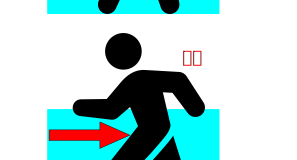
\includegraphics[width=.5\textwidth]{pool_walking.png}
			\end{center}
		\end{minipage}
		\caption{プールでの水中歩行}
		\label{pool_walk}
	\end{center}
\end{figure}

このことから、液体\index{えきたい@液体}の性質として、変形させる速度が変わると生じる力も変わって、速い変形に対しては応力も大きくなることがわかります。


\subsection{液体\index{えきたい@液体}の力学モデル}

\subsubsection{ ニュートンの法則}
では、液体\index{えきたい@液体}の力学的な応答を記述するモデルはどうなるのでしょうか。
これは、古典力学の土台を築いた Sir Isaac Newton が、流れのせん断応力\index{せんだん@せん断応力} $\tau$ とせん断速度\index{せんだん@せん断速度} $\dot{\gamma}$ (速度勾配\index{そくどこうばい@速度勾配})との間に比例関係を見出しています。

実際の実験は、図 \ref{nijyu} に示したような二重になった円筒中に試料となる液体\index{えきたい@液体}を入れ、内部の円筒を回転させながらそのときに生じる力を測定します。
内部に入った円筒の回転速度を変化させることでせん断速度\index{せんだん@せん断速度}を変化させ、そのときに生じるせん断応力との間に比例関係があることを見出しました。

この比例関係を式で表せば、
	\begin{align}
		\text{せん断応力} &= \text{比例定数} \times \text{せん断速度} \notag \\
		\tau &= \eta \dot{\gamma}
	\end{align}
式中で示した比例定数が、物質の流れ易さを表す指標である「粘度\index{ねんど@粘度}」となります。
\begin{figure}[htb]
	\begin{center}
		\begin{minipage}{0.6\textwidth}
			\large
			\begin{itembox}[l]{ニュートンの法則}
				\vspace{-3mm}
				\begin{align*}
					\text{せん断応力} &= \text{比例定数} \times \text{せん断速度} \notag \\
					\tau &= \eta \dot{\gamma}
				\end{align*}
				比例定数 $\eta$ が、物質の流れ易さを表す「粘度\index{ねんど@粘度}」
			\end{itembox}
		\end{minipage}
		\begin{minipage}{0.3\textwidth}
			\begin{center}
			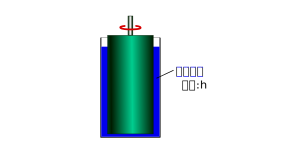
\includegraphics[width=.8\textwidth]{nijyu_entou.png}
			\end{center}
		\end{minipage}
		\caption{二重円筒による測定}
		\label{nijyu}
	\end{center}
\end{figure}

なお、粘度\index{ねんど@粘度}の単位は以下のようになります。
\begin{align}
	[\text{粘度}] &= \dfrac{[\text{せん断応力}]}{[\text{せん断速度}]} \notag \\
		&= \dfrac{[\mathrm{Pa}]}{[\mathrm{s^{-1}}]} = [\mathrm{Pa\cdot s}]
\end{align}


\subsubsection{液体\index{えきたい@液体}の力学モデル}

ニュートンの法則が成り立つような液体\index{えきたい@液体}の力学モデルをイメージ図とすると、図 \ref{flow_model} となります。
\begin{figure}[htbp]
	\begin{center}
		\begin{minipage}{0.55\textwidth}
			\large
			\begin{itembox}[l]{液体のモデル}
				\begin{itemize}
					\item 液体の振る舞いを表すモデル
					\item 右図のダッシュポット
					\item イメージとしては、水鉄砲
					\item 速くピストンを動かすと、\\抵抗が大。
				\end{itemize}
			\end{itembox}
			
		\end{minipage}
		\begin{minipage}{0.35\textwidth}
			\begin{center}
			\includegraphics[width=.8\textwidth]{dashpot.png}
			\end{center}
		\end{minipage}
		\caption{液体の力学モデル}
		\label{flow_model}
	\end{center}
\end{figure}

このモデルは、液体\index{えきたい@液体}の抵抗がその変形速度に比例するというニュートン流体の特性を表しています。

\section*{この章のまとめ}

この章では、固体と液体という基本的な物質のふるまいを書き表す一番単純なモデルについて、説明を進めました。
	\begin{boxnote}
		\large
		\begin{itemize}
			\item 固体と液体という基本的な物質のありようについて、レオロジー的に考えていきます。
			\begin{itemize}
				\item 固体の最も基本的なモデルである弾性体という状態
				\item 刺激と応答を表すために、ひずみと応力を使うことで力学モデルが書けること
				\item 液体の応答について
				\item 液体の力学モデルが、「ひずみ速度\index{ひずみそくど@ひずみ速度}」で表されること
			\end{itemize} 
		\end{itemize}
	\end{boxnote}

	\newpage

	\begin{longartdeco}
		\begin{center}
		\emph{コラム:カエルの話}	
		\end{center}
	
		早逝されてしまった、元レオロジー学会長の上田さんという方がレオロジーの学び方のポイントとして、カエルの話をしていました。せっかくなので残して行きたいなと思い、ここに書いておくことにします。

	最初の話は、「茹でガエル」というもので、環境変化に関する寓話です。
	これは、1960年代の東西冷戦、1980年代の終末論、1990年代には温暖化に関連して取り上げられてきているようです。

	2つ目の話は、イソップ寓話に収録されている「二匹のカエル」というお話で、困難な状況でも頑張れば道は開ける(かも)というものです。
	上田さんは強引にクリームのダイラタンシーの話にしてレオロジーとつなげていました。
	結局、どっちのやり方がいいのかは、結果を見るまではわからないということなんで、自分のやり方を信じるしかないですね。

	「茹でガエル」

	カエルのような変温動物は、外部の温度環境によって自身の温度が変化します。
	したがって、本来は、気温が高くなって暑い場合は冷たい場所へ、また、気温が下がって凍えるときには暖かい場所へと移動する必要があります。
	カエルを熱い湯の中に入れてみると、居心地の良い場所へと慌てて逃げ出して行きます。
	でも、カエルを水の入ったビーカーに入れてゆっくりと水の温度を上げていくと、カエルは周りの温度が上がったことに気づかなくて、そのまま茹で上がって死んでしまいます。
	と書きましたが、これは似非科学的な作り話とのことです。

	人間も周りの環境が徐々に変化していっても気づかなくて、「アッと気づいたとき」には、逃げようのないとんでもない状況に追い込まれることがあります。
	ここから転じて、以下のような警句を表しています。
	「現状認識をしっかりと!」
	これは、周囲の変化に対して、常にきちんと対応しましょうということですね。

	「二匹のカエル」

	二匹のカエルが、ミルクのいっぱい入った壺の縁の周りを飛び跳ねていましたが、突然、二匹とも壺に落ちてしまいました。
	一匹のカエルは、「ああ、もう駄目だー!」と諦めてしまって、じっとして、結局溺れて死んでしまいました。
	もう一日のカエルは、「なんとかしよう」ともがいて、何度も何度も足を蹴って一生懸命泳ぎました。すると、足元のミルクがだんだんとチーズになって固まってきて、それを足がかりにして壺の外へと飛び出せました。
	これから得られる警句は、
	「現状分析するよりも行動を!」
	ということになります。
	まあ、変に周りが見えると、小賢しい考えにとらわれるので良くない場合もあるということです。
	
	\end{longartdeco}

\end{document}
\clearpage
\section*{}
\addcontentsline{toc}{section}{演習問題}    
\input{chap_3_Ensyu.tex}

\chapter{物質の物理を理解するために}
\documentclass[uplatex,dvipdfmx,a4paper,11pt]{jsarticle}

\usepackage{docmute}


% 数式
\usepackage{amsmath,amsthm,amssymb}
\usepackage{bm}
% 画像
\usepackage{graphicx}

\usepackage{multirow}
\usepackage{wrapfig}
\usepackage{ascmac}
\usepackage{xcolor}


\usepackage{makeidx}
\makeindex

\graphicspath{{../../Figures//}{../../Figures/Rheology/}}

\usepackage{qrcode}
\setlength\lineskiplimit{0pt}
\setlength\normallineskiplimit{0pt}

\usepackage{qexam}

\usepackage{titlesec}
\titleformat*{\section}{\Large\bfseries}
\titleformat*{\subsection}{\large\bfseries}
\titleformat*{\subsubsection}{\normalsize\bfseries}
\titleformat*{\paragraph}{\normalsize\bfseries}

% ページ設定
% \pagestyle{empty}
% 高さの設定
\setlength{\textheight}{\paperheight}   % ひとまず紙面を本文領域に
\setlength{\topmargin}{-5.4truemm}      % 上の余白を20mm(=1inch-5.4mm)に
\addtolength{\topmargin}{-\headheight}  % 
\addtolength{\topmargin}{-\headsep}     % ヘッダの分だけ本文領域を移動させる
\addtolength{\textheight}{-40truemm}    % 下の余白も20mmに%% 幅の設定
\setlength{\textwidth}{\paperwidth}     % ひとまず紙面を本文領域に
\setlength{\oddsidemargin}{-5.4truemm}  % 左の余白を20mm(=1inch-5.4mm)に
\setlength{\evensidemargin}{-5.4truemm} % 
\addtolength{\textwidth}{-40truemm}     % 右の余白も20mmに
% 図と本文との間
%\abovecaptionskip=-5pt
%\belowcaptionskip=-5pt
%
% 全体の行間調整
% \renewcommand{\baselinestretch}{1.0} 
% 図と表
%\renewcommand{\figurename}{Fig.}
%\renewcommand{\tablename}{Tab.}
%

% \makeatletter 
% \def\section{\@startsection {section}{1}{\z@}{1.5 ex plus 2ex minus -.2ex}{0.5 ex plus .2ex}{\large\bf}}
% \def\subsection{\@startsection{subsection}{2}{\z@}{0.2\Cvs \@plus.5\Cdp \@minus.2\Cdp}{0.1\Cvs \@plus.3\Cdp}{\reset@font\normalsize\bfseries}}
% \makeatother 

\usepackage[dvipdfmx,%
 bookmarks=true,%
 bookmarksnumbered=true,%
 colorlinks=false,%
 setpagesize=false,%
 pdftitle={数式に頼らない直感的理解による材料設計のためのレオロジー⼊⾨},%
 pdfauthor={佐々木裕},%
 pdfsubject={},%
 pdfkeywords={レオロジー; 材料設計; }]{hyperref}
\usepackage{pxjahyper}

\usepackage{plext}

\usepackage{niceframe} 
\usepackage{framed}
\newenvironment{longartdeco}{%
  \def\FrameCommand{\fboxsep=\FrameSep \artdecoframe}%
  \MakeFramed {\FrameRestore}}%
 {\endMakeFramed}
 
\usepackage{siunitx}

\newcommand{\rmd}{\mathrm{d}}

\usepackage[inline]{showlabels}

\begin{document}

\section*{この章の内容}

具体的なレオロジーの議論に入る前に、もう少しだけ、レオロジーに関する物理モデルを理解するために必要となる数学と物理の基礎的な事項について確認していきましょう。
ここでは、前章よりは少し難しい話になり、高校から大学レベルのお話をすることになります。

まず、レオロジーに関する物理モデルを作っていくときに必要となる2つの関数を説明し、続いて、その数学的な議論をすすめるための微分方程式を解けるように微分と積分という考え方について、そのイメージの部分だけを概観していきます。
また、その物理モデルを我々が取り扱いたい物質の物理へとつなげるために、力とポテンシャルの関係についても微積分を利用して理解を深めていきます。

具体的な事項を以下に列記しました。
\begin{boxnote}
	\large
	\begin{itemize}
		\item レオロジーで扱う関数について
		\begin{itemize}
			\item 指数関数と対数関数について
		\end{itemize}
		\item 微積分について
		\begin{itemize}
			\item 微積分について
			\item 簡単な微分方程式の解き方
		\end{itemize} 
		\item 物理モデルを物質の物理とつなげるために
		\begin{itemize}
			\item 力、仕事、ポテンシャルと微積分
			\item 摩擦と熱について
		\end{itemize} 
	\end{itemize}
\end{boxnote}

\section{レオロジーで扱う関数について}

\subsection{関数の一覧}

以前に、関数\index{かんすう@関数}について簡単に触れて、物理的なイメージを得るためには線型\index{せんけい@線型}性が成り立つような範囲で議論するとかんたんにモデル化できるということをお話しました。
これは関数としては、一次関数ということになります。
確かに、線型\index{せんけい@線型}関係に持ち込めれば単純化できて便利なのですが、事象の関係はそう単純に進むわけでもありません。

様々な関数\index{かんすう@関数}について、表 \ref{kansu} に一覧にまとめました。
何もここで、数学的に面倒なお話をするつもりはありませんが、これらの関数も当然使いみちがあり非常に有用なのです。
その位置づけを確認する意味で、少し違う観点で、初等関数というものを確認します。
実用的に簡単に言いきってしまえば、高校までの数学で習った範囲での関数ということになります。

\begin{itembox}[l]{Wikipedia での「初等関数」の説明}
	初等関数とは、\href{https://ja.wikipedia.org/wiki/%E5%88%9D%E7%AD%89%E9%96%A2%E6%95%B0#:~:text=%E5%88%9D%E7%AD%89%E9%96%A2%E6%95%B0%EF%BC%88%E3%81%97%E3%82%87%E3%81%A8%E3%81%86%E3%81%8B%E3%82%93%E3%81%99%E3%81%86,%E3%81%AA%E3%81%A9%E3%81%AF%E5%88%9D%E7%AD%89%E9%96%A2%E6%95%B0%E3%81%A7%E3%81%AA%E3%81%84%E3%80%82}{Wikipedia の「初等関数」} によれば、「実数または複素数の1変数関数で、代数関数、指数関数、対数関数、三角関数、逆三角関数および、それらの合成関数を作ることを有限回繰り返して得られる関数のことである。」と書かれています。

	% なお、\href{https://ja.wikipedia.org/wiki/%E9%96%A2%E6%95%B0_(%E6%95%B0%E5%AD%A6)}{Wikipedia の「関数(数学)」} の真ん中あたりに、多様な関数をクラス分けした見やすい表があります。
\end{itembox}

代数関数というのも本来の定義はちょっと面倒ですが、中学程度で習った多項式関数(一次関数、二次関数、等\footnote{
	その他に、分数関数、無理関数があります。
})をイメージしていただければいいと思います。

レオロジーを理解するために必要となる関数\index{かんすう@関数}としては、よく使われるものとして、指数関数\index{しすうかんすう@指数関数}と対数関数\index{たいすうかんすう@対数関数}を挙げることができます。
ここでは、その2つについて簡単に確認します。

\begin{table}[tb]
	\begin{center}
		\caption{様々な関数}
		\label{kansu}
		\begin{tabular}{|c|c|c|c|c|c|} \hline
			\multicolumn{5}{|c|}{関数} &	具体例 \\ \hline
			\multirow{11}{*}{ \pbox<t>{初等関数} } & \multirow{6}{*}{ \pbox<t>{代数関数} } & \multirow{5}{*}{ \pbox<t>{有理関数} } & \multirow{4}{*}{ \pbox<t>{多項式関数} }	&	定数関数	& $f(x) = a$	\\ \cline{5-6}
			&&&& 一次関数	& $f(x) = ax + b$	\\ \cline{5-6}
			&&&& 二次関数	& $f(x) = ax^2 + bx + c$ \\ \cline{5-6}
			&&&& 三次関数	& $f(x) = ax^3 + bx^2 + cx + d$	\\ \cline{4-6}
			&&& \multicolumn{2}{c|}{分数関数}	& $f(x) = \dfrac{a}{x}$	\\ \cline{3-6}
			&& \multicolumn{3}{c|}{無理関数}	& $f(x) = \sqrt{x}$	\\ \cline{2-6}
			& \multirow{5}{*}{ \pbox<t>{初等超越関数} } & \multicolumn{3}{c|}{指数関数}	& $f(x) = e^x$	\\ \cline{3-6}
			&& \multicolumn{3}{c|}{対数関数}	& $f(x) = \ln (x)$	\\ \cline{3-6}
			&& \multicolumn{3}{c|}{三角関数}	& $f(x) = \sin x$	\\ \cline{3-6}
			&& \multicolumn{3}{c|}{双曲線関数}	& $f(x) = \sinh x$	\\ \cline{3-6}
			&& \multicolumn{3}{c|}{冪関数}	& $f(x) = x^a$	\\ \hline
			\multirow{4}{*}{ \pbox<t>{特殊関数} } & \multicolumn{4}{c|}{ガンマ関数}	& $\Gamma (x)$	\\ \cline{2-6}
			& \multicolumn{4}{c|}{ベータ関数}	& B$(x,y)$	\\ \cline{2-6}
			& \multicolumn{4}{c|}{誤差関数}	& $erf(x)$	\\ \cline{2-6}
			& \multicolumn{4}{c|}{デルタ関数}	& $\Delta$	\\ \hline
		\end{tabular}
	\end{center}
\end{table}


\subsection{指数関数\index{しすうかんすう@指数関数}について}

\subsubsection{指数関数の定義}
指数関数\index{しすうかんすう@指数関数}を天下りに定義すると、「指数関数とは、冪における指数\index{しすう@指数}を変数として、その定義域を主に実数の全体へ拡張して定義される初等超越関数の一種である。」というように書かれています。
このような定義だけもみても具体的なイメージがわかりにくいので、まず、キーワードとして「冪(ベキとよみます。)」と、累乗の説明も合わせて示しました。
\large
\begin{itembox}[l]{「指数関数」の天下りな定義}
	「指数関数とは、冪における指数\index{しすう@指数}を変数として、その定義域を主に実数の全体へ拡張して定義される初等超越関数の一種である。」
	\begin{align*}
		f(x) = a^x
	\end{align*}
	\begin{itemize}
		\item 冪とは
		\begin{itemize}
			\item 「底」と呼ばれる正の数の右肩に「指数」と呼ばれる数を載せた数式表現であり、指数\index{しすう@指数}が自然数の場合に累乗と呼ばれる。
		\end{itemize}
		\item 累乗
		\begin{itemize}
			\item 「累」= 重ねる、「乗」= 掛ける\\
			したがって、累乗は複数回掛け合わせるということを意味します。
		\end{itemize}
		\begin{equation*}
			\underbrace{a\times a\times a \cdots \times a}_{\text{$n$個}} = a^n
		\end{equation*}
	\end{itemize}
\end{itembox}
\normalsize

\subsubsection{指数\index{しすう@指数}の性質}
指数\index{しすう@指数}の性質を簡単にまとめると以下のようになります。
\large
\begin{itembox}[l]{指数\index{しすう@指数}の性質}
	\begin{itemize}
		\item 累乗同士の掛け算は、指数同士の足し算 $a^n \times a^m = a^{(n+m)}$
		\item 累乗のさらなる累乗は、指数同士の掛け算 $(a^n)^m = a^{(n \times m)}$
		\item 指数が 0 の場合は? $a^0 = 1$
		\item 指数が負 $\Rightarrow$ 指数が正の逆数 $a^{-k} = \dfrac{1}{a^k}$
		\item 指数同士の割り算は指数の引き算 $a^n \div a^m = a^{n-m}$
		\item 指数が分数の場合
			\begin{itemize}
				\item 分数の分母となる値を用いて累乗根を表し、
				\item 分子はそのべき乗を表す\\
				$a^{\frac{m}{n}}=\sqrt[n]{a^m}$
			\end{itemize}
	\end{itemize}
\end{itembox}
\normalsize
上記のような性質を天下りに暗記してもいいのですが、指数\index{しすう@指数}が自然数だけで定義される「累乗としての性質」を確認した上で、その声質をベースとして、指数\index{しすう@指数}を整数、そして、有理数へと拡張して、性質の由来を確認していきましょう。

このように、限定的な条件で成立した性質を基礎として、条件をより広い範囲へと広げてその声質を確認していくような考え方は、物理モデル\index{ぶつりもでる@物理モデル}を考えるときにも非常に役に立ちます。
できれば、自分の手を動かして確認してみてください。

\paragraph{指数\index{しすう@指数}が自然数の場合}
まず、指数\index{しすう@指数}が自然数の場合に限定して、議論しましょう。

同じ底の累乗同士の掛け算は、
\begin{align*}
a^n \times a^m 	&= (\underbrace{a\times a\times a \cdots \times a}_{\text{$n$個}}) \times (\underbrace{a\times a\times a \cdots \times a}_{\text{$m$個}}) \notag \\
		&= \underbrace{a\times a\times a \cdots \times a}_{\text{$n+m$個}} \notag \\
		&= a^{(n+m)}
\end{align*}
となり、指数同士の足し算となります。

また、累乗のさらなる累乗は、
\begin{align*}
(a^n)^m 	&= \underbrace{(\underbrace{a\times a \cdots \times a}_{\text{$n$個}}) \times (\underbrace{a\times a \cdots \times a}_{\text{$n$個}}) \cdots \times (\underbrace{a\times a \cdots \times a}_{\text{$n$個}})}_{\text{$m$}個} \notag \\
		&= \underbrace{a\times a\times a \cdots \times a}_{\text{$n \times m$個}} \notag \\
		&= a^{(n \times m)}
\end{align*}
この場合は、指数\index{しすう@指数}同士の掛け算となります。

さらに、異なる底の累乗同士の掛け算は指数\index{しすう@指数}が同一の場合にだけ可能であり、
\begin{align*}
a^n \times b^n 	&= (\underbrace{a\times a\times a \cdots \times a}_{\text{$n$個}}) \times (\underbrace{b\times b\times b \cdots \times b}_{\text{$n$個}}) \notag \\
		&= \underbrace{(a \times b) \times (a \times b) \cdots \times (a \times b)}_{\text{$n$個}} \notag \\
		&= (a \times b)^n
\end{align*}
というように底同士の掛け算としてまとめることができます。

指数\index{しすう@指数}が自然数であった場合の、累乗に関する公式は以上の三つとなります。

\paragraph{整数への拡張}
これから、指数の定義域を拡張して行きましょう。
これ以降の拡張は、上記の基本となる累乗の三つの公式を満たすように拡張して行くことになります。

指数の定義域を整数へと拡張するために、最初に、$a \ne 0(a^n\ne0)$ としておいて、指数が0の場合($a^0$)を考えましょう。
累乗同士の掛け算の関係式を用いると、
\begin{align*}
a^n \times a^0 =a^{(n+0)} = a^n 
\end{align*}
$a^n \ne 0$であるので、上式の両辺を$a^n$で除して、
\begin{equation*}
a^0 = 1
\end{equation*}
が得られます。

これを、指数が0の場合($a^0$)の定義として表現すると、「$a \ne 0$ である任意の実数 $a$ について,$a^0 = 1$ が成り立つ」とということになります
\footnote{
なお、$a = 0$ のときは、$0^0$ は不定となるため、考えないこととします。
}。

さらに、負の数への拡張として、$k$ が正の整数だった場合の、$a^{-k}$ について考えてみましょう。
\begin{equation*}
a^k \times a^{-k} = a^{k+(-k)}=a^0=1
\end{equation*}
最後の変換で、上記の指数が 0 の定義を用いています。
そして、$a^k$ で両辺を除すと、
\begin{equation*}
a^{-k} = \dfrac{1}{a^k}
\end{equation*}
結局、指数が負の場合は、指数が正であった場合の逆数となるように定義することができます。

このとき、指数同士の割り算を考えれば、以下のように指数の引き算となります。
\begin{equation*}
a^n \div a^m =a^n \times \dfrac{1}{a^m} = a^n \times a^{-m} = a^{n + (-m)}
\end{equation*}

\paragraph{有理数への拡張}
最後に、分数(有理数)にまで拡張しましょう。
この拡張は、特別なことを定義する必要もなく、指数が分数の場合においても、これまでに示してきたような指数の公式に基づいて計算を行うということになります。

指数が分数の場合として、$a^{m/n}$(ただし、$n$、$m$は整数)というものを考えると、この累乗は、
\begin{equation*}
(a^{\frac{m}{n}})^n=a^{\frac{m}{n} \times n}=a^m
\end{equation*}
すなわち、$a^{m/n}$ の $n$ 乗が $a^m$ となると考えることができます。

ここで、一般には、実数 $x$ に対して $x$ を $n$ 乗すると $y$ になるとき($n$ は正の整数)、$y$ を「$x$ の $n$ 乗根」と呼び、$\sqrt[n]{x}$ と表記するのでした。

この関係を用いると、上記の指数が分数の場合は、指数となる分数の分母となる値を用いて累乗根を表し、以下のように記述できることになります。
\begin{equation*}
a^{\frac{m}{n}}=\sqrt[n]{a^m}
\end{equation*}

\paragraph{指数関数\index{しすうかんすう@指数関数}の特徴}
独立変数として実数である $x$ を指数とする関数を、一般に指数関数と呼びます。
\begin{equation*}
f(x)=a^x
\end{equation*}

$y=a^x$としたとき、 $xy$平面上でのグラフは以下の特徴を持っています。

物理的な議論においては、底としてネイピア数$e$を用いる場合が非常に多くなります
\footnote{ネイピア数$e$は、$\pi$と同様に多用される数学定数の一つであり、その値は、$e=2.718281828 \cdots $と続く「超越数」です。}。
ここでは、底が $e$ の場合を、独立変数を見やすくするために、$\exp (x)$ と表記します。
\begin{figure}[htb]
	\begin{center}
		\begin{minipage}{0.45\textwidth}
			\large
			\begin{itembox}[l]{指数関数の特徴}
				\begin{itemize}
					\item \textcolor{red}{$\exp (x)$ は、単調増加。}
					\item \textcolor{green}{$\exp (-x) = \left(\dfrac{1}{e} \right)^x$ は、\\単調減少。}
					\item 常に、点$(0,1)$を通る。
					\item $x$軸($y=0$)を漸近線
				\end{itemize}
			\end{itembox}
		\end{minipage}
		\begin{minipage}{0.45\textwidth}
			\begin{center}
			\includegraphics[width=\textwidth]{exp.png}
			\end{center}
		\end{minipage}
		\caption{指数関数の特徴}
		\label{fig: exp(x)}
	\end{center}
\end{figure}

指数関数 $y = \exp (x)$ のグラフを、図 \ref{fig: exp(x)} に示しました。
$x=0$ において $y=1$ であり、$x$ の増加に伴い単調増加し、$x=1$ では $y=e$ となっています。
指数が負である場合は単調減少となるが、いずれの場合も、関数の値は正となります。

\subsection{対数関数\index{たいすうかんすう@対数関数}について}

\subsubsection{対数関数とは}
対数関数\index{たいすうかんすう@対数関数}とは、指数関数\index{しすうかんすう@指数関数}とは表裏一体であり、逆関数となっています。
この関係を、図 \ref{shisuu_taisuu} に示しました。
\begin{figure}[htb]
	\begin{center}
		\begin{minipage}{0.45\textwidth}
			\large
			\begin{itembox}[l]{指数関数と対数関数}
				\vspace{-3mm}
				\begin{align*}
					\textcolor{blue}{a}^{\textcolor{red}{x}} = \textcolor{green}{M} \Leftrightarrow \textcolor{red}{x}= \log_{\textcolor{blue}{a}} \textcolor{green}{M}
				\end{align*}
				\begin{itemize}
					\item 指数関数:底に指数を作用させて真数を求める関数
					\item 対数関数:真数は底にどんな指数を与えたものかを求める関数
					\item $y = x$ のグラフに関して対称
				\end{itemize}
			\end{itembox}
		\end{minipage}
		\begin{minipage}{0.45\textwidth}
			\begin{center}
			\includegraphics[width=\textwidth]{exp_ln.png}
			\end{center}
		\end{minipage}
		\caption{指数関数と対数関数の関係}
		\label{shisuu_taisuu}
	\end{center}
\end{figure}

\subsubsection{対数\index{たいすう@対数}の性質}
対数関数\index{たいすうかんすう@対数関数}の性質を以下にまとめました。
これらの性質は、指数関数のものと同様に導出できますので、ここでは一覧として示すだけにします。
一度自分の手を動かして導出されることをお勧めします。
\large
\begin{itembox}[l]{対数関数の性質}
	任意の正の実数である $M,N$ に対して、
			\begin{itemize}
				\item 対数同士の足し算は、真数の掛け算 $\ln (M \times N) = \ln M + \ln N$
				\item 対数同士の引き算は、真数の割り算 $\ln(M \div N) = \ln M - \ln N$
				\item 真数の冪は、冪を掛け算に $\ln M^p = p \ln M$
				\item 真数の逆数は、マイナスを付けて $\ln \dfrac{1}{M} = -\ln M$
				\item $\ln 1 = 0$
			\end{itemize}
\end{itembox}
\normalsize
対数関数は、大きな数を桁数でざっくりと見るときに便利であるという特徴があり、線弾性スペクトルのように極端に範囲の広いデータを取り扱うときに使用されます。

\subsubsection{対数\index{たいすう@対数}グラフ}
対数\index{たいすう@対数}のもう一つの有用な使いみちとして、グラフにおける軸を対数表示するという対数グラフというものがあり、一つの軸のみを対数表示した「片対数グラフ\index{かたたいすう@片対数グラフ}」と、両方の軸を対数化した「両対数グラフ\index{りょうたいすう@両対数グラフ}」があります。

\paragraph{片対数\index{かたたいすう@片対数}グラフ}
片対数グラフ\index{かたたいすう@片対数グラフ}とは、一つの軸のみを対数表示したものとなります。

指数関数で表される数式があったとき、両辺の対数\index{たいすう@対数}を取ると、以下のように展開できます。
\begin{align*}
	y&=\exp(ax+b) \\
	\therefore \; \ln y &= ax + b
\end{align*}

このとき、縦軸を対数目盛としたグラフにプロットすれば、その傾きが $a$、$y$ 切片が $b$ となる直線が得られるわけです。

\begin{figure}[htb]
	\begin{center}
		\begin{minipage}{0.45\textwidth}
			\large
			\begin{itembox}[l]{片対数グラフの例}
				\begin{itemize}
					\item 指数関数を取り扱う際に、
					\item 両辺の対数を取ると、\\
					$\ln y = ax + b$
					\begin{itemize}
						\item 関数値の対数が、
						\item 変数の1次関数となる。
						\item 指数が傾きとして求まる。
					\end{itemize}
				\end{itemize}
			\end{itembox}
		\end{minipage}
		\begin{minipage}{0.45\textwidth}
			\begin{center}
			\includegraphics[width=\textwidth]{relux_6.png}
			\end{center}
		\end{minipage}
		\caption{片対数グラフの例}
		\label{fig:semilog}
	\end{center}
\end{figure}

\paragraph{両対数\index{りょうたいすう@両対数}グラフ}
両対数グラフ\index{りょうたいすう@両対数グラフ}とは、両方の軸を対数で表示したものです。
\begin{figure}[htb]
	\begin{center}
		\large
		\begin{minipage}{0.45\textwidth}
			\begin{itembox}[l]{両対数グラフの意味}
				\begin{itemize}
					\item 極端に範囲の広いデータを扱えるため、粘弾性スペクトルは、通常この形で表される。
					\item 冪関数 $y = x^a$ を線型で処理できる。
					\begin{align*}
						\log y = a \log x
					\end{align*}
					両対数グラフにプロットすれば、その傾きが決まる。
				\end{itemize}
			\end{itembox}
		\end{minipage}
		\begin{minipage}{0.45\textwidth}
			\begin{center}
			\includegraphics[width=\textwidth]{beki.png}
			\end{center}
		\end{minipage}
		\caption{両対数グラフの例}
		\label{fig:loglog}
	\end{center}
\end{figure}

\section{微積分\index{びせきぶん@微積分}について}

\subsection{微分\index{びぶん@微分}について}
微分とは、「対象とする関数\index{かんすう@関数}が、注目したい点の周りでどのように振る舞うのかを、明らかにする方法」と考えることができます。

\subsubsection{微分\index{びぶん@微分}の考え方}
微分の直感的なイメージとしては、注目する点における関数の振る舞いを接線の傾きで表したものと考えることができます。
\begin{figure}[htb]
	\begin{center}
		\begin{minipage}{0.5\textwidth}
			\large
			\begin{itembox}[l]{微分の直感的説明}
				\begin{itemize}
					\item 注目する点近傍での、接線の「傾き」
					\begin{itemize}
						\item 変数の増分と、
						\item 関数の増分との比
					\end{itemize}
					\item 変数の増分を無限小にしたとき、
				\end{itemize}
			\end{itembox}
		\end{minipage}
		\begin{minipage}{0.4\textwidth}
			\begin{center}
			\includegraphics[width=\textwidth]{bibun.jpeg}
			\end{center}
		\end{minipage}
		\caption{微分の考え方}
		\label{bibun}
	\end{center}
\end{figure}

関数 $f(x)$ を $x$ で微分することを、$\dfrac{\mathrm{d} f(x)}{\mathrm{d}x}$ と書き表します。
ここでの、d が微小量の変化であることを表し、「分母である変数」と「分子となっている関数」との「僅かな変化の比」をとるイメージとなっています。

\large
	\begin{itembox}[l]{微小な変化の比}
		\begin{itemize}
			\item 関数 $f(x)$ を $x$ で微分することを、
			\item $\dfrac{\mathrm{d} f(x)}{\mathrm{d}x}=\dfrac{\text{関数の微小変化量}}{変数の微小変化量}$ 
			\begin{itemize}
				\item ``d'' が微小量の変化であることを表し、
				\item 「分母である変数」と「分子となっている関数」との「僅かな変化の比」
			\end{itemize}
		\end{itemize}
	\end{itembox}
\normalsize

\subsubsection{微分のイメージ}
もう少しだけ、直感的な理解につながるアナロジーを考えていきましょう。

自転車の発電式(ダイナモ)ライトを例に取ってみます。

\begin{figure}[htb]
	\begin{center}
		\begin{minipage}{0.5\textwidth}
			\large
			\begin{itembox}[l]{自転車のライトの例}
				\begin{itemize}
					\item 速度を上げると明るく、止まると\\消える。
					\begin{itemize}
						\item 明るさが瞬間的な速度
						\item 微分の値の大小に対応
					\end{itemize}
					\item 明るさ $\Leftrightarrow$ 非常に短い時間あたりに\\進める距離
				\end{itemize}
			\end{itembox}
		\end{minipage}
		\begin{minipage}{0.4\textwidth}
			\begin{center}
			\includegraphics[width=.8\textwidth]{bike.jpg}
			\end{center}
		\end{minipage}
		\caption{自転車のライトの例}
		\label{bike_light}
	\end{center}
\end{figure}

このアナロジーからも、微分で見ることで関数の瞬間的な振る舞いを見ることができるとわかります。
\begin{itemize}
	\item 微分大 $\Leftrightarrow$ その瞬間に変化量が大きい
	\item 微分小 $\Leftrightarrow$ その瞬間にはあまり変化しない。
\end{itemize}

\subsubsection{微分\index{びぶん@微分}の公式}
微分の公式には様々なものがありますが、今回の講座として取り扱う微分に関する公式は、表 \ref{bibun_kousiki} に示したようなものぐらいです。

\renewcommand{\arraystretch}{2}
\begin{table}[tb]
	\begin{center}
		\caption{微分の公式}
		\label{bibun_kousiki}
			\begin{tabular}{|c|c|c|} \hline
				微分の対象		& 公式							& メモ \\ \hline \hline
				冪の微分		& $\dfrac{\mathrm{d}}{\mathrm{d}x}x^a = ax^{a-1}$ 		&  多項式では線形性も利用\\ \hline
				指数関数の微分	& $\dfrac{\mathrm{d}}{\mathrm{d}x}\exp(x) = \exp(x)$ 		&  ネイピア数の場合\\ \hline
				自然対数の微分	& $\dfrac{\mathrm{d}}{\mathrm{d}x}\ln x = \dfrac{1}{x}$ 	& 底がネイピア数 \\ \hline
			\end{tabular}
		\end{center}
\end{table}
\renewcommand{\arraystretch}{1.}

\subsection{積分\index{せきぶん@積分}について}
積分には、大きく分けて2つの使い方があります。
一つは、定積分と呼ばれる、処理する範囲を定めて計算するやり方であり、イメージとしては関数が占める範囲を面積として表すような考え方ということになり、もう一つは、不定積分と呼ばれる処理の範囲を定めることなく数式の変換を行うものであり、微分\index{びぶん@微分}の逆変換というイメージで捉えることができます。

\subsubsection{定積分\index{ていせきぶん@定積分}について}
まず、定積分についての説明から始めます。

定積分が表すものは、直感的には、指定した範囲における、関数 $f(x)$ が表す曲線と $x$ 軸との間の「面積」と考えることができます。
この面積を求めるために、変数の微小な刻み $\mathrm{d} x$ と、その点近傍での関数 $f(x)$ との積 $f(x) \mathrm{dx}$(これは、グラフの短冊の部分の面積にあたります)を指定した範囲に渡って積算することになります。
\begin{figure}[htb]
	\begin{center}
		\begin{minipage}{0.45\textwidth}
			\large
			\begin{itembox}[l]{定積分の考え方}
				\begin{itemize}
					\item 直感的には「面積」
					\begin{itemize}
						\item \textcolor{green}{微小な刻み $\mathrm{d} x$} と
						\item \textcolor{red}{$f(x)$} との積(面積:\\グラフの短冊)を
						\item \textcolor{blue}{積算}する。
					\end{itemize}
					\vspace{-3mm}
					\small
					\begin{align*}
						\left[ F(x) \right]_a^b = \textcolor{blue}{\int_a^b} \textcolor{red}{f(x)} \textcolor{green}{\mathrm{d} x}
					\end{align*}
				\end{itemize}
			\end{itembox}
		\end{minipage}
		\begin{minipage}{0.45\textwidth}
			\begin{center}
			\includegraphics[width=.8\textwidth]{integral.png}
			\end{center}
		\end{minipage}
		\caption{定積分のイメージ}
		\label{sekibun}
	\end{center}
\end{figure}

この積算するということを、和(Summation)を表すギリシア記号 $\sum$ から、その頭文字の ``S'' を流用して縦方向に長く伸ばしたものである、インテグラル $\int$ という積分記号で表しているのです。そして、どの範囲を積分するのかということを積分記号の上と下に示します。
\large
\begin{itembox}[l]{自動車の移動の例}
	\begin{itemize}
		\item 速度が時間 $t$ の関数として $v(t)$ で表されるとき、
		\item 時刻 $t_0$ から $t_1$ までに進んだ距離 $L$ は、
	\end{itemize} 
	\begin{align*}
		L=\int_{t_0}^{t_1} v(t) \mathrm{d} t
	\end{align*}
\end{itembox}
\normalsize

\subsubsection{不定積分\index{ふていせきぶん@不定積分}について}
つぎに、不定積分として、微分の逆変換を行うことについての説明に進みます。

不定積分とは、積分範囲を定めない(不定)積分処理を行うことにより、微分するとその関数 $f(x)$ に一致するような関数(原始関数と呼ばれます)$F(x)$ を求める操作ということができます。
したがって、積分を微分の逆操作だととして考えると、不定積分により求めた式の両辺を微分すれば、元の関数が出てくることになるわけです。

なお、この処理において、定数 $C$ (積分定数)の分だけ不定値が出ることになります。

\large
\begin{itembox}[l]{微分の逆操作としての不定積分}
	\begin{itemize}
		\item 微分するとその関数 $f(x)$ に一致するような
		\item 原始関数 $F(x)$ を求める操作
		\begin{itemize}
			\item 積分範囲を定めない(不定)
			\item このとき、定数 $C$ (積分定数)だけ不定値が出る。
		\end{itemize}
			\begin{align*}
				F(x) = \int f(x) \mathrm{d} x +C
			\end{align*}
		\item (逆操作)両辺を微分すれば、元の関数
			\begin{align*}
				\dfrac{\mathrm{d}}{\mathrm{d} x} F(x) = f(x)
			\end{align*}
	\end{itemize}
\end{itembox}
\normalsize

\subsection{微積分\index{びせきぶん@微積分}とは}

では、微積分\index{せきぶん@積分}を使うことの意味について考えていきます。

微分を使うことで、任意の瞬間における関数の振る舞いの描像を取り出すことができます。
そして、積分を行うことで、注目する範囲全体に渡る関数の振る舞いの結果を総量として把握できるようになるのです。

\large
	\begin{itembox}[l]{微積分を使うこととは?}
		\begin{itemize}
			\item 微分で瞬間の描像を取り出し、
			\item 積分で全体のふるまいを総量として把握。
		\end{itemize}
	\end{itembox}
\normalsize

別の観点で考えると、小学校の算数においては、物事の変化が一定の値に従って(平均値で)生じていると考えて、単純に割り算や掛け算で処理していたわけです。
しかしながら、実際の振る舞いは瞬間ごとに異なる場合が多いので、単純な計算では対処できなくなります。
そのときに、微分や積分の出番となるわけです。
\begin{figure}[htb]
	\begin{center}
		\includegraphics[width=.8\textwidth]{biseki.png}
		\caption{微分と積分の関係}
		\label{fig:biseki}
	\end{center}
\end{figure}

\subsection{簡単な微分方程式\index{びぶんほうていしき@微分方程式}}
やっと、微積分に関する準備が整いましたので、「物理モデル\index{ぶつりもでる@物理モデル}」を数学的に記述する際に必要となる「微分方程式」というものにお話を進めます。

\subsubsection{微分方程式\index{びぶんほうていしき@微分方程式}とは}
微分方程式とは、「物理現象や化学現象を、微分の形で記述したもの」であり、微分の逆操作である積分を用いることで解くことができます。
これを使いこなすことで、注目する現象の振る舞いをわかりやすい関数で表すことができるようになるわけです。
\large
	\begin{itembox}[l]{微分方程式とは?}
		「物理現象や化学現象を、微分の形で記述したもの」
			\begin{itemize}
				\item 例えば、「放射性物質の崩壊」等の、一次反応と呼ばれる化学現象を記述する頻出の微分方程式の形
				\begin{align*}
					\textcolor{red}{\dfrac{\mathrm{d}}{\mathrm{d} t} N(t)} = \textcolor{blue}{-aN(t)}
				\end{align*}
				\item この式の意味は、
				\begin{itemize}
					\item 左辺は\textcolor{red}{時間の関数である $N(t)$ の時間変化を微分の形}、
					\item 右辺はその変化が、\textcolor{blue}{$N(t)$ の量に比例して減少(負号がついているから)}することを表す。
					\item 定数 $a$ は [1/T] の次元を持つ。
				\end{itemize}
				\item \textbf{「積分\index{せきぶん@積分}を使って、方程式を解く。」}
			\end{itemize}
	\end{itembox}
\normalsize

\subsubsection{簡単な微分方程式の解き方の例}
微分方程式の解き方として、「変数分離」というものがあります。
これは、微分方程式の中で用いられている変数を、それぞれ、一方の辺に集めてしまうことを意味しています。
そして、微分量である $\mathrm{d}y$ や、$\mathrm{d}t$ を、演算可能な量を表すものとして扱います。

この解き方を用いて、上述の一次反応を表す微分方程式を実際に説いてみましょう。
\large
	\begin{itembox}[l]{一次反応を表す微分方程式を解いてみましょう}
		\textbf{1st step: }方程式の両辺に $\rmd t$ を掛ける。
		\begin{align*}
			\dfrac{1}{N} \mathrm{d}N= -a\mathrm{d} t
		\end{align*}

		\textbf{2nd step: }方程式の両辺に積分記号 $\int$ をつける。
		\begin{align*}
			\int \dfrac{1}{N} \rmd N = -a \int \mathrm{d} t
		\end{align*}

		\textbf{3rd step: }両辺の不定積分\index{ふていせきぶん@不定積分}を計算する。
		\begin{align*}
			\ln N +C_1 = -at + C_2
		\end{align*}

		\textbf{4th step: }積分定数を一つ($C=C_2-C_1$)にまとめる。
		\begin{align*}
			\ln N = -at + C
		\end{align*}

		\textbf{5th step: }指数関数\index{しすうかんすう@指数関数}に書き直してから、指数の性質を使って定数項を書き直し($C'=\exp(C)$)。
		\begin{align*}
			N=\exp(-at + C) = \exp(C) \times \exp(-at) = C' \exp(-at)
		\end{align*}

		これで、微分方程式としては一旦解けたことになるが、初期条件を考慮すれば定数項を定めることができる。
		$t=0$ での初期濃度が $N_0$ とすると、$\exp(-a*0) = 1$ であることを用いて、
		\begin{align*}
			&N(t=0) = C' \exp(-a*0) = N_0 \\
			\therefore\; &C' = N_0
		\end{align*}

		\textbf{Final step: }上記の定数項を用いて、濃度は時間の関数として以下となる。
		\begin{align*}
			N(t) = N_0 \exp(-at)
		\end{align*}
	\end{itembox}
\normalsize

ここで現れた指数関数の形が、レオロジーの物理モデルでも頻出であることについては、後ほど「粘弾性での応力緩和」の議論において示します。

\subsubsection{指数関数\index{しすうかんすう@指数関数}的な減少について}

定数として定めた $a$ は、[1/T] という時間の逆数の次元を持っていました。
これを、時間の次元を持った $1/\tau$ と書き換えると、前述の濃度変化を表す式は以下となります。
\begin{align*}
	N(t) = N_0 \exp \left(-\dfrac{t}{\tau} \right)
\end{align*}

この濃度変化を表す式をグラフに表すと、図 \ref{fig:exp_kanwa} となります。
\begin{figure}[htb]
	\begin{center}
		\begin{minipage}{0.45\textwidth}
			\large
			\begin{itembox}[l]{指数関数的減少とは}
				\begin{itemize}
					\item 濃度変化を表す式をグラフに表すと、右図となる。
					% \begin{align*}
					% 	N(t) = N_0 \exp \left(-\dfrac{t}{\tau} \right)
					% \end{align*}
					\item 時間経過に伴い濃度が減少し $t = \tau$ において
					\begin{align*}
						N(\tau) 
						&= N_0 \exp(-1)\\ 
						&= \dfrac{N_0}{e}
					\end{align*}
				\end{itemize}
			\end{itembox}
		\end{minipage}
		\begin{minipage}{0.45\textwidth}
			\begin{center}
			\includegraphics[width=\textwidth]{relux_1.png}
			\end{center}
		\end{minipage}
		\caption{指数関数的減少と緩和時間}
		\label{fig:exp_kanwa}
	\end{center}
\end{figure}

グラフから、時間の次元を持つ $\tau$ は、初期濃度の $\dfrac{1}{e}$ となる時間であることがわかります。
この、指数関数の時間に伴う現象を表す特徴的な時間を「緩和時間\index{かんわじかん@緩和時間}」と呼びます。
\large
	\begin{itembox}[l]{緩和時間とは}
		\begin{itemize}
			\item 時間の次元を持つ $\tau$ は、初期濃度の $\dfrac{1}{e}$ となる時間を表します。
			\item この特徴的な時間を「緩和時間」と呼びます。
		\end{itemize}
	\end{itembox}	
\normalsize

\subsubsection{緩和時間\index{かんわじかん@緩和時間}についてもう少し}

緩和時間\index{かんわじかん@緩和時間}の意味について、もう少し考察をしてみましょう。

濃度変化は以下の式で書けるのでした。
\begin{align*}
	N(t) = N_0 \exp \left(-\dfrac{t}{\tau} \right)
\end{align*}

この濃度の式を時間で微分すると、減少速度は以下の式となります。
\begin{align*}
	\dfrac{\mathrm{d}N(t)}{\mathrm{d}t} = -\dfrac{N_0}{\tau} \exp \left(-\dfrac{t}{\tau} \right)
\end{align*}

したがって、$t=0$ での減少速度は、以下となります。
\begin{align*}
	\dfrac{\mathrm{d}}{\mathrm{d}t}N(0) &=-\dfrac{N_0}{\tau} \exp \left(-\dfrac{0}{\tau} \right) \\
	&=-\dfrac{N_0}{\tau}
\end{align*}

結局、初期状態($t=0$)での減少速度を維持して濃度が減少したとすれば、緩和時間 $\tau$ だけ時間経過したときに濃度が 0 となることになります。
\begin{figure}[htb]
	\begin{center}
		\begin{minipage}{0.45\textwidth}
			\large
			\begin{itembox}[l]{緩和時間のもう一つの意味}
				\begin{itemize}
					\item 初期速度を維持して濃度が\\減少すると、
					\item $t=\tau$ で濃度が 0
				\end{itemize}
			\end{itembox}
		\end{minipage}
		\begin{minipage}{0.45\textwidth}
			\begin{center}
			\includegraphics[width=\textwidth]{relux_2.png}
			\end{center}
		\end{minipage}
		\caption{緩和時間のもう一つの意味}
		\label{fig:exp_kanwa2}
	\end{center}
\end{figure}

\section{物理モデルを物質の物理とつなげるために}

ここでは、「物理モデル\index{ぶつりもでる@物理モデル}」として仮想的にイメージできるモデルを実際の物質での物理とつなげていくために、力、仕事、エネルギーという大事な物理量を確認します。
その理解の上で、物質のマクロ及びミクロでの状態を記述するポテンシャルと力の関係が微積分でつながっていることを見て行きます。

\subsection{仕事\index{しごと@仕事}、エネルギー\index{えねるぎー@エネルギー}}

まず、最初に、仕事とエネルギーの確認から始めましょう。

仕事とは、「質点に力\index{ちから@力}を作用して、移動すること」であり、物理量としては、「仕事 $W$ は、作用させた力 $F$ と移動した距離 $s$ の積」として定義されます。
\begin{align*}
	W=F \times s
\end{align*}
\begin{figure}[htb]
	\begin{center}
		\begin{minipage}{0.42\textwidth}
			\large
			\begin{itembox}[l]{仕事とは}
				\begin{itemize}
					\item 質点に力を作用して、移動すること
					\item 仕事は、作用させた力 $F$ と移動した距離 $s$ の積
				\end{itemize}
					\includegraphics[width=.8\textwidth]{work.png}
			\end{itembox}
		\end{minipage}
		\begin{minipage}{0.42\textwidth}
			\large
			\begin{itembox}[l]{エネルギーとは}
				\begin{itemize}
					\item 仕事をする能力のこと
					\item 物体や空間(場)は、その状態を変えることによりエネルギーを蓄える。
					\item 仕事とエネルギーの次元は同一。
				\end{itemize}
			\end{itembox}
		\end{minipage}
		\caption{仕事とエネルギー}
		\label{fig:work_energy}
	\end{center}
\end{figure}



エネルギー\index{えねるぎー@エネルギー}は、「仕事\index{しごと@仕事}をする能力」のことであり、仕事とエネルギーの次元は同一となっています。
したがって、物体や空間(場)は、力学的な仕事を受けることでその状態を変えることによりエネルギーが高い状態となり、エネルギーを蓄えることになります。
\large
\begin{itembox}[l]{仕事とエネルギーの次元と組み立て単位}
	\begin{itemize}
		\item 次元:[仕事] = [力][距離] = [$ML^2T^{-2}$]
		\item 組み立て単位:ジュール J
	\end{itemize}
\end{itembox}
\normalsize

レオロジーにおいては、外力\index{がいりょく@外力}に対応して物質が変形したとき、静力学的な釣り合いのもとで物質が仕事をされたと考えることができます。
言い換えれば、外力\index{がいりょく@外力}が物質の内部に蓄積された(弾性\index{だんせい@弾性})エネルギーに相当する量の仕事を行ったことになります。

\subsection{ポテンシャル\index{ぽてんしゃる@ポテンシャル}と力\index{ちから@力}と微積分\index{びせきぶん@微積分}}
次に、ポテンシャルについて考えましょう。
\large
\begin{itembox}[l]{ポテンシャルとは?}
	\begin{itemize}
		\item 基準の状態を定めて、
		\begin{itemize}
			\item その着目する状態にするために、
			\item その物体あるいは空間に加えた仕事の量
		\end{itemize}
		\item 逆に言えば
		\begin{itemize}
			\item ある状態から基準の状態に戻るまでに、
			\item 外に取り出すことのできるエネルギーの量
		\end{itemize}
		\item 力が「\textcolor{red}{保存力}」であれば、
		\item ポテンシャルが「位置のみの関数の\textcolor{red}{状態量}」となる
	\end{itemize}
	\begin{screen}
		\begin{itemize}
			\item 保存力\index{ほぞんりょく@保存力}:仕事が経路によらないように定義できる力
			\item 状態量:系の状態だけで、一意に決まる物理量
		\end{itemize}
	\end{screen}
\end{itembox}
\normalsize

ポテンシャル\index{ぽてんしゃる@ポテンシャル}とは、「任意の基準の状態を定めたうえで、着目する状態にするためにその物体あるいは空間に加えた仕事の量」と定義することができます。
このことを逆に言えば、「ある状態から基準の状態に戻るまでに外に取り出すことのできるエネルギー\index{えねるぎー@エネルギー}の量」と考えることもできます。

このとき、対象としている環境の違いが重要となります。
力が「保存力\index{ほぞんりょく@保存力}」であれば、ポテンシャルは「位置のみの関数として与えられる状態量」となるのですが、実際の物質ではそうならない場合もよく生じてしまいます。
このことについては、次の項目で説明します。
\begin{figure}[htb]
	\begin{center}
		\begin{minipage}{0.4\textwidth}
			\large
			\begin{itembox}[l]{ポテンシャル $U(\bm{r})$は、}
				\begin{itemize}
					\item 基準の位置 $\bm{r_0}$ から、
					\item 位置 $\bm{r}$ までの、
					\item 力 $F(\bm{r})$ の積分
				\end{itemize}
				\vspace{-3mm}
				% \small
				\begin{align*}
					W(\bm{r}) = \int_{\bm{r_0}}^{\bm{r}} F(\bm{r}) \rmd \bm{r} = -U(\bm{r})
				\end{align*}
			\end{itembox}
			\begin{itembox}[l]{力 $F(\bm{r})$は、}
				\begin{itemize}
					\item 任意の位置で、
					\item $U(\bm{r})$ を微分すれば、
				\end{itemize}
				\vspace{-3mm}
				% \small
					\begin{align*}
						\dfrac{\mathrm{d}}{\mathrm{d}\bm{r}} U(\bm{r}) = -F(\bm{r})
					\end{align*}
			\end{itembox}
		\end{minipage}
		\begin{minipage}{0.5\textwidth}
			\begin{center}
			\includegraphics[width=.9\textwidth]{potential_power.png}
			\end{center}
		\end{minipage}
		\caption{ポテンシャルと力と微積分}
		\label{fig:pot_power}
	\end{center}
\end{figure}

力\index{ちから@力}を保存力として考えられる、理想的な状態においてもう少し整理します。

ポテンシャル\index{ぽてんしゃる@ポテンシャル}は、基準の位置 $\bm{r_0}$ から、任意の位置 $\bm{r}$ までの、力 $F(\bm{r})$ の積分として以下のように書けます。

	\begin{align*}
		W(\bm{r}) = \int_{\bm{r_0}}^{\bm{r}} F(\bm{r}) \rmd \bm{r} = -U(\bm{r})
	\end{align*}

逆に言えば、任意の位置でポテンシャル $U(\bm{r})$ を微分すれば、その位置での力を算出することができ、結局、表裏一体の逆変換として捉えることができるわけです。
\begin{align*}
	\dfrac{\mathrm{d}}{\mathrm{d}\bm{r}} U(\bm{r}) = -F(\bm{r})
\end{align*}



\subsection{摩擦力\index{まさつりょく@摩擦力}、非保存力\index{ひほぞんりょく@非保存力}}

この節の最後に、現実の世界に少し近づいてみましょう。

ここまでの議論の大半は、力が保存力であり仕事\index{しごと@仕事}やポテンシャルが状態料として考えられる、高校までの物理で取り扱っていた理想的(仮想的)な状態での議論でした。
実際の我々の周りで生じている事象は、そんなに単純ではなく、ものを移動させようとすると摩擦という抵抗が生じてきます。
\begin{figure}[htb]
	\begin{center}
		\begin{minipage}{0.45\textwidth}
			\large
			\begin{itembox}[l]{摩擦と熱}
				\begin{itemize}
					\item 摩擦力は非保存力
						\begin{itemize}
							\item ポテンシャルは状態量ではなく経路に依存
						\end{itemize}
					\item 内部の粒子の摩擦により、
						\begin{itemize}
							\item 粒子の運動エネルギーが増加し系全体の温度が上昇
							\item 非断熱系では、熱エネルギーとして外界に散逸。
						\end{itemize}
					\item 非保存力も含めれば、系全体のエネルギーは保存
				\end{itemize}
			\end{itembox}
		\end{minipage}
		\begin{minipage}{0.45\textwidth}
			\begin{center}
			\includegraphics[width=\textwidth]{thermal_eng.png}
			\end{center}
		\end{minipage}
		\caption{摩擦力、熱}
		\label{fig:masatsu_netsu}
	\end{center}
\end{figure}

摩擦力は非保存力であり、摩擦を考慮した系においては、ポテンシャルは状態量ではなく経路に依存することになります。
摩擦が生じる原因については、これも細かく考えていくとややこしくなってきますので、ここでは現実に生じているものだということで詳細には立ち入りません。

ただ、レオロジー的に考えるときに、次の章で議論するような内部の粒子\index{りゅうし@粒子}を想定してモデルを設定すると、粒子同士の摩擦により、粒子\index{りゅうし@粒子}の運動エネルギー\index{ねつえねるぎー@運動エネルギー}が増加し系全体の温度が上昇するという状態をイメージすることができます。
このようにして発生した熱が、断熱していない系では、熱エネルギー\index{ねつえねるぎー@熱エネルギー}として外界に散逸することになります。

このような非保存力も含めて考えれば、系全体のエネルギーは保存することになります。
図 \ref{fig:masatsu_netsu} には、保温した容器の中の水を撹拌することにより、熱が仕事と等価であることを示したジュールの実験装置の概略を示しました。

\section*{この章のまとめ}

この章では、具体的なレオロジーの議論に入る前に、これからの議論に必要となる数学と物理の基礎的な事項について、高校から大学レベルの内容を確認しました。
\begin{boxnote}
	\large
	\begin{itemize}
		\item 数学的な事項について
			\begin{itemize}
				\item レオロジーで扱う関数について、指数関数とその逆関数に対応する対数関数の確認
				\item 微積分について、微分が「瞬間的な振る舞いを記述」し、積分が「全体の量を把握」する
				\item 簡単な微分方程式をとくことで、レオロジー関連の事項で頻出の「指数関数的な応答」を理解
			\end{itemize}
		\item 物理に関する事項として
			\begin{itemize}
				\item 次元について、「次元解析」や「無次元量」について
				\item 力、仕事、ポテンシャルを確認して、その微積分との関係について
			\end{itemize}
	\end{itemize}
\end{boxnote}

\newpage

\begin{longartdeco}
	\begin{center}
	\emph{コラム:「褒めて育てる」?}	
	\end{center}

	著者は、「地声も大きく、気も短くて、かつ、物事を曖昧にしておくのが苦手」なので、つい、いろんなことを確認のつもりでポンポンと根掘り葉掘り聞いてしまいます。
	この態度が、年下の人に対する圧迫的な振る舞いに見えるようで、あなたはパワハラ体質ですねとよく指摘されてしまいます。
	「叱って指導しても人は育ちません」と諭されてしまうことも度々でした。
	
	「部下は褒めて育てる。」ということが、最近のトレンドになっています。
	確かに、人は叱られるよりは褒められたほうが気持ちがいいので、「北風よりは太陽」を好みます。
	そのような環境のほうがのびのびと仕事が進むはずでしょう。
	
	でも、この「褒めるマネージメント」が、いつもうまくいくかというとそういうわけでもないようです。
	例えば、部下の方が褒められそうな行動を前もって予測して、そのような行動だけを取るようになってしまう場合もよく見かけます。
	その結果として、上司の耳あたりの良いことだけを選んで報告して都合の悪いことは無視(隠して)してしまうこともあります。
	これでは、自主性もなく、上司の気持ちだけを「忖度する部下」を養成しているのかもしれません。
	一見できる部下という、ちょっと世渡りの下手な(出来の悪いとされがちな)人よりもたちの悪い、本当に困った部下を作り出す環境なのかもしれません。
	
	ということで、どちらの方法でも、うまく行かないことが多いわけです。
	見方を変えてみると、叱るにしても、褒めるにしても、上司(あなた)の主観、判断、都合が入っているわけです。
	では、どうすればいいのでしょうか?
	
	この境目が、「きちんと承認する」ということになるのかもしれません。
	きちんと目の前にある事実から目をそらすことなく、自身の思い込みだけに頼ることなく、あるがままの状態を一旦そのままで受け入れてから、
	その「あるべき状態を想像しながら対応する。」という態度が、一番公平な対応ではないでしょうか。
	
	これって、結局、(中立的に)科学的な態度で目の前の事象に対応するということになるわけです。
	そのうえで、コミュニケーションの基本である「相手に自身の認識を正しく伝える」ということを愚直に行えばいいのでしょう。
	この対応が、上記の「きちんと承認する」という行為になるので、中立的な表現として受け手(部下)にシンプルに伝わることが期待できます。
	
	ということで、「科学的なアプローチをきちんと行った上で、コミュニケーション能力の向上に少しだけ努力するというあたりが一番妥当な道かな?」と思う今日この頃です。


\end{longartdeco}


\end{document}
\clearpage
\section*{}
\addcontentsline{toc}{section}{演習問題}    
\input{chap_4_Ensyu}

\chapter{物理化学として物質を見直すと}
\documentclass[uplatex,dvipdfmx,a4paper,11pt]{jsarticle}

\usepackage{docmute}


% 数式
\usepackage{amsmath,amsthm,amssymb}
\usepackage{bm}
% 画像
\usepackage{graphicx}

\usepackage{multirow}
\usepackage{wrapfig}
\usepackage{ascmac}
\usepackage{xcolor}


\usepackage{makeidx}
\makeindex

\graphicspath{{../../Figures//}{../../Figures/Rheology/}}

\usepackage{qrcode}
\setlength\lineskiplimit{0pt}
\setlength\normallineskiplimit{0pt}

\usepackage{qexam}

\usepackage{titlesec}
\titleformat*{\section}{\Large\bfseries}
\titleformat*{\subsection}{\large\bfseries}
\titleformat*{\subsubsection}{\normalsize\bfseries}
\titleformat*{\paragraph}{\normalsize\bfseries}

% ページ設定
% \pagestyle{empty}
% 高さの設定
\setlength{\textheight}{\paperheight}   % ひとまず紙面を本文領域に
\setlength{\topmargin}{-5.4truemm}      % 上の余白を20mm(=1inch-5.4mm)に
\addtolength{\topmargin}{-\headheight}  % 
\addtolength{\topmargin}{-\headsep}     % ヘッダの分だけ本文領域を移動させる
\addtolength{\textheight}{-40truemm}    % 下の余白も20mmに%% 幅の設定
\setlength{\textwidth}{\paperwidth}     % ひとまず紙面を本文領域に
\setlength{\oddsidemargin}{-5.4truemm}  % 左の余白を20mm(=1inch-5.4mm)に
\setlength{\evensidemargin}{-5.4truemm} % 
\addtolength{\textwidth}{-40truemm}     % 右の余白も20mmに
% 図と本文との間
%\abovecaptionskip=-5pt
%\belowcaptionskip=-5pt
%
% 全体の行間調整
% \renewcommand{\baselinestretch}{1.0} 
% 図と表
%\renewcommand{\figurename}{Fig.}
%\renewcommand{\tablename}{Tab.}
%

% \makeatletter 
% \def\section{\@startsection {section}{1}{\z@}{1.5 ex plus 2ex minus -.2ex}{0.5 ex plus .2ex}{\large\bf}}
% \def\subsection{\@startsection{subsection}{2}{\z@}{0.2\Cvs \@plus.5\Cdp \@minus.2\Cdp}{0.1\Cvs \@plus.3\Cdp}{\reset@font\normalsize\bfseries}}
% \makeatother 

\usepackage[dvipdfmx,%
 bookmarks=true,%
 bookmarksnumbered=true,%
 colorlinks=false,%
 setpagesize=false,%
 pdftitle={数式に頼らない直感的理解による材料設計のためのレオロジー⼊⾨},%
 pdfauthor={佐々木裕},%
 pdfsubject={},%
 pdfkeywords={レオロジー; 材料設計; }]{hyperref}
\usepackage{pxjahyper}

\usepackage{plext}

\usepackage{niceframe} 
\usepackage{framed}
\newenvironment{longartdeco}{%
  \def\FrameCommand{\fboxsep=\FrameSep \artdecoframe}%
  \MakeFramed {\FrameRestore}}%
 {\endMakeFramed}
 
\usepackage{siunitx}

\newcommand{\rmd}{\mathrm{d}}

\usepackage[inline]{showlabels}

\begin{document}

\section*{この章の内容}

この章では、物質の三態(固体、液体、気体)という最も基本的な「ものの有り様」について、物理化学的に⾒直していきます。

まず、固体を粒子が整列した結晶モデルでイメージして、その弾性体としての力の起源がどのように生じているのかを理解します。
そして、液体が流れるということを、マクロな変形が粒子モデルでのミクロな移動にどのようにつながるかというイメージを深めたうえで、
固体と液体の違い、さらには、その間に存在するガラス状態を理解していきます。

最後に、刺激の応答としての応⼒がどのように発⽣するのかということについて、固体の場合と液体の場合のそれぞれのあり方をイメージできるようにします。

具体的に列記すると、以下のような事項となります。
\begin{boxnote}
	\large
    \begin{itemize}
		\item 物質の三態について
		\begin{itemize}
			\item 固体のモデルとしての結晶
			\item 液体のモデル
		\end{itemize} 
		\item 流れるということは?
		\begin{itemize}
			\item マクロな変形と粒子の移動
			\item 固体と液体の境目
			\item ガラス状態
		\end{itemize} 
		\item 応力の由来は?
		\begin{itemize}
			\item 結晶の応力の起源
			\item 液体の応力とは?
		\end{itemize}
	\end{itemize}
\end{boxnote}

\section{物質の三態について}

\subsection{物質の三態}
物質の状態は、その相の違いによって固体\index{こたい@固体}、液体\index{えきたい@液体}、気体の3つに分類できます。
これから、その由来について考えていきましょう。
\begin{figure}[htb]
	\begin{center}
		\begin{minipage}{0.4\textwidth}
			\large
			\begin{itembox}[l]{マクロとミクロに考えて、}
				\begin{itemize}
					\item マクロな視点では?
					\begin{itemize}
						\item 気体、液体 ⇔ 流れる
						\item 固体 ⇔ 流れない
					\end{itemize}
					\item ミクロに中身を考えると、\\何が違うのでしょうか?
				\end{itemize}
			\end{itembox}
		\end{minipage}
		\begin{minipage}{0.5\textwidth}
			\begin{center}
			\includegraphics[width=\textwidth]{3Phase.png}
			\end{center}
		\end{minipage}
		\caption{物質の三態について}
		\label{fig:santai}
	\end{center}
\end{figure}

\subsubsection{ミクロとマクロ}
歴史的に考えると、物質の状態は人間が手で触って実感できるようなマクロな性質に従って、分類されてきました。
すなわち、固体\index{こたい@固体}は定まった体積と形を持つ物体であり、一方、液体\index{えきたい@液体}は体積を減少させるように押しつぶすことは困難ですが、
形は自由に変化します。
そして、気体では圧縮することもできるので体積も形も定まっていないという性質を持っています。

雰囲気温度が変化すれば、それに応じて、物質はこの三態の間を移ろっていきます。
物質が置かれている環境の温度を低下させれば、気体は凝集して液体\index{えきたい@液体}となり、液体\index{えきたい@液体}は凝固して固体\index{こたい@固体}となります。
逆に、固体\index{こたい@固体}を温度が高い状態とすれば融解して液体\index{えきたい@液体}になり、さらなる加熱により液体\index{えきたい@液体}が蒸発して気体へと変化します。

この三態の振る舞いをレオロジー的に考えると、「流れるかどうか」ということが重要なポイントになります。
すなわち、液体\index{えきたい@液体}と固体\index{こたい@固体}との明白な相違点は流れるかどうかということに集約されるわけです。

そして、「流れるという現象」を考えていく場合には、物質の内部のミクロな状態を考える必要が出てきます。
ミクロな視点に立った場合に、流れるという現象はどのように考えることができるのでしょうか。

\subsection{固体\index{こたい@固体}のモデルとしての結晶}
まず、出発点として、固体\index{こたい@固体}のモデルを考えていきましょう。

前述のように、固体\index{こたい@固体}の特徴は流れないということでした。
この特性は、ミクロにはどのようなモデルとして考えれば理解できるのでしょうか。

\subsubsection{結晶のモデル}
マクロに見た固体\index{こたい@固体}を具体的に考えると、金属、塩、鉱物(石)、セラミックス(陶器)、ガラス、木材、等々に分類されます。
これらの物質は、その成り立ちが違うため、それを構成する物質の組成も全く異なったものとなっています。

簡略化して取り扱うために、中学や高校で習ったような物理化学の範囲においては思い切った単純化を行って、
固体\index{こたい@固体}は何らかの粒子\index{りゅうし@粒子}(原子や分子)が規則的に並んだ「結晶としてモデル化」されてきました。

\begin{figure}[htb]
	\begin{center}
		\includegraphics[width=.9\textwidth]{crystals.png}
		\caption{結晶という固体の模式図}
		\label{fig:crystals}
	\end{center}
\end{figure}

\subsubsection{二粒子間のポテンシャル}

個体を、粒子\index{りゅうし@粒子}が規則的に整列することによって構成されたと考える結晶構造としてモデル化した場合、
マクロに見たときの「流れないという性質」は、ミクロに見れば粒子間に強い相互作用が働いているということに対応します。
つまり、粒子間に隣の粒子\index{りゅうし@粒子}を引き止めるような力が働いているおかげで、マクロな性質である形状維持して流れないという特性が生じていると
考えるわけです。
\begin{figure}[htb]
	\begin{center}
		\begin{minipage}{0.4\textwidth}
			\large
			\begin{itembox}[l]{固体の性質をミクロに}
				\begin{itemize}
					\item 固体には、マクロな\\「流れないという性質」
					\item ミクロに見れば、粒子間に強い相互作用が必要
				\end{itemize}
			\end{itembox}
		\end{minipage}
		\begin{minipage}{0.5\textwidth}
			\begin{center}
			\includegraphics[width=.8\textwidth]{ryusi_1.png}
			\end{center}
		\end{minipage}
		\caption{固体を構成する粒子同士の相互作用}
		\label{fig:ryusi}
	\end{center}
\end{figure}

この粒子間の相互作用\index{そうご@相互作用}については、多様な検討が行われ、これまでに多数のモデルが提案されてきています。
その一つがよく使用されている Lennard-Jones ポテンシャル\index{れなーどじょーんずぽてんしゃる@Lennard-Jones ポテンシャル}というものになります。
\begin{figure}[htb]
	\begin{center}
		\begin{minipage}{0.4\textwidth}
			\large
			\begin{itembox}[l]{Lennard-Jones ポテンシャル}
				\begin{itemize}
					\item 速く消失する\textcolor{red}{斥力}
					\item 遠くまで働く\textcolor{blue}{引力}
					\item \textcolor{green}{それらの和}で相互作用
				\end{itemize}
				\begin{align*}
					U(r) = 4 \epsilon \left[ \textcolor{red}{\left(\dfrac{\sigma}{r} \right)^{12}} - \textcolor{blue}{\left(\dfrac{\sigma}{r} \right)^{6}} \right]
				\end{align*}
			\end{itembox}
		\end{minipage}
		\begin{minipage}{0.5\textwidth}
			\begin{center}
			\includegraphics[width=\textwidth]{LJ_potential.png}
			\end{center}
		\end{minipage}
		\caption{Lennard-Jones ポテンシャル}
		\label{fig:Lennard-Jones}
	\end{center}
\end{figure}

これは、相対的に速く消失する斥力と遠くまで働く引力との和として二体間の相互作用\index{そうご@相互作用}を書き表したポテンシャルです。
\begin{align*}
	U(r) = 4 \epsilon \left[ \left(\dfrac{\sigma}{r} \right)^{12} - \left(\dfrac{\sigma}{r} \right)^{6} \right]
\end{align*}

以前に示したように、ポテンシャル\index{ぽてんしゃる@ポテンシャル}を微分\index{びぶん@微分}すれば、力\index{ちから@力}を表す式が得られるのでした。
したがって、上式を微分することで、粒子間に働く力 $F(r)$ がわかります。
\begin{align*}
	\begin{cases}
		U(r) = 4 \epsilon \left[ \left(\dfrac{\sigma}{r} \right)^{12} - \left(\dfrac{\sigma}{r} \right)^{6} \right] \\
		F(r) = -\dfrac{\rmd}{\rmd r}U(r) = 4 \epsilon \left[ 12 \left(\dfrac{\sigma^{12}}{r^{13}} \right) - 6 \left(\dfrac{\sigma^6}{r^7} \right) \right]
	\end{cases}
\end{align*}

このとき、ポテンシャルが極小値となるところ(ポテンシャルの井戸とも呼ぶ)において、二粒子間に働く力が 0 となっていることがわかります。
\begin{figure}[htb]
	\begin{center}
		\begin{minipage}{0.4\textwidth}
			\large
			\begin{itembox}[l]{ポテンシャルの微分で力を}
				\normalsize
				\begin{align*}
					\begin{cases}
						U(r) &= 4 \epsilon \left[ \left(\dfrac{\sigma}{r} \right)^{12} - \left(\dfrac{\sigma}{r} \right)^{6} \right] \\[10pt]
						F(r) &= -\dfrac{\rmd}{\rmd r}U(r) \\[10pt]
						&= 4 \epsilon \left[ 12 \left(\dfrac{\sigma^{12}}{r^{13}} \right) - 6 \left(\dfrac{\sigma^6}{r^7} \right) \right]
					\end{cases}
				\end{align*}
			\end{itembox}
		\end{minipage}
		\begin{minipage}{0.5\textwidth}
			\begin{center}
				\includegraphics[width=.8\textwidth]{LJ_pot_Force.png}
			\end{center}
		\end{minipage}
		\caption{ポテンシャルの微分で力を導出}
		\label{fig:LJ_pot_Force}
	\end{center}
\end{figure}

この二粒子間に働いている力について、もう少し詳しく見てみましょう。

ポテンシャル\index{ぽてんしゃる@ポテンシャル}の極小値($r \simeq 1.16$)において二粒子間の力\index{ちから@力}は 0 となり、粒子間の距離がそれ以上に短くなると力が正となりますから、
斥力が働くことになります。
また、粒子\index{りゅうし@粒子}がその釣り合いの位置から離れすぎると力が負で引力が働きます。
これらの相互作用\index{そうご@相互作用}の結果として、二粒子間の距離がほぼ定まって、ポテンシャルの井戸の近傍に存在することが安定状態であることがわかります。
\begin{figure}[htb]
	\begin{center}
		\begin{minipage}{0.45\textwidth}
			\large
			\begin{itembox}[l]{二粒子間の力}
				\begin{itemize}
					\item 粒子の近接では斥力
					\item 離れすぎると引力
					\item その結果として、二粒子間の\\距離がほぼ定まる
				\end{itemize}
			\end{itembox}
		\end{minipage}
		\begin{minipage}{0.45\textwidth}
			\begin{center}
			\includegraphics[width=.8\textwidth]{LJ_pos.png}
			\end{center}
		\end{minipage}
		\caption{二粒子間に働く力}
		\label{fig:lj-pos}
	\end{center}
\end{figure}

\subsubsection{多体問題として考えると、}
結晶のモデルにおいては、粒子\index{りゅうし@粒子}の相互作用\index{そうご@相互作用}は二体間に限るわけではなく、多数の粒子が相互作用\index{そうご@相互作用}を生じています。
この多体問題をきちんと解くことは大変なのですが、簡略化して安定状態を考えることもそれほど的外れではありません。
\begin{figure}[htb]
	\begin{center}
		\begin{minipage}{0.55\textwidth}
			\large
			\begin{itembox}[l]{多体系での相互作用}
				\begin{itemize}
					\item 多体の相互作用を簡略化して、
					\item 二体間の相互作用に基づくとすれば、
					\item 多体の粒子が安定距離の近傍で摂動
				\end{itemize}
			\end{itembox}
		\end{minipage}
		\begin{minipage}{0.35\textwidth}
			\begin{center}
			\includegraphics[width=.6\textwidth]{LJ_ryusi.png}
			\end{center}
		\end{minipage}
		\caption{簡略化した多体系の安定状態}
		\label{fig:tatai}
	\end{center}
\end{figure}

多体の相互作用\index{そうご@相互作用}を簡略化して、二体間の相互作用\index{そうご@相互作用}の単純な重ね合わせに基づくと仮定すれば、結局、
多体の粒子\index{りゅうし@粒子}が二体間相互作用の安定距離の近傍で摂動することになります。

\subsubsection{固体\index{こたい@固体}のミクロなイメージ}

二体間のポテンシャル\index{ぽてんしゃる@ポテンシャル}を用いることで、結晶モデルとして固体\index{こたい@固体}を形成する粒子の振る舞いの理解が少しだけ進みました。
ここでは、分子動力学シミュレーションという方法を使って、もう少し直感的なイメージを膨らましてみましょう。
なお、分子動力学シミュレーションの説明は以下にまとめた程度に控え、詳細は割愛します。
\large
\begin{itembox}[l]{分子動力学シミュレーションとは}
	\begin{itemize}
		\item 粒子の描像で物理現象をシミュレートする方法
		\item それぞれの粒子の運動は、ニュートン力学に従って算出する。
		\item 系の温度が粒子の揺動となる。
		\item 粒子の間に適切なポテンシャルを設定(今回は、LJ ポテンシャル)する。
	\end{itemize}
\end{itembox}
\normalsize

分子動力学シミュレーションにより、粒子間相互作用として LJ ポテンシャルを設定し、十分に低温にして固体\index{こたい@固体}における粒子の振る舞いをシミュレートした結果を、図 \ref{fig:MD-kotai} に示しました。

\begin{figure}[htb]
	\begin{center}
		\begin{minipage}{0.48\textwidth}
			\large
			\begin{itembox}[l]{固体のシミュレーション}
				\begin{itemize}
					\item T=0.1 (十分に低温な状態)
					\item 面心立方になるように、初期の\\粒子を配置。
					\item 分子動力学シミュレーションを\\実施。
					\item 動的な運動を見ても、粒子の\\動きが殆ど見られない。
				\end{itemize}
			\end{itembox}
		\end{minipage}
		\begin{minipage}{0.42\textwidth}
			\begin{center}
			\includegraphics[width=\textwidth]{N1_FCC.png}
			\large
			\begin{screen}
				\begin{itemize}
					\item これはスナップショット
					\item 動画でも殆ど動いていない。
				\end{itemize}
			\end{screen}
			\end{center}
		\end{minipage}
		\caption{固体の分子動力学シミュレーション}
		\label{fig:MD-kotai}
	\end{center}
\end{figure}

このシミュレーションの結果として、十分に低温とした場合には粒子\index{りゅうし@粒子}の運動は抑制され、ポテンシャルの井戸の底に対応する場所でわずかに摂動する程度のものであることが確認できます。


\subsection{固体\index{こたい@固体}と液体\index{えきたい@液体}}
ここまでの議論で、固体\index{こたい@固体}のミクロなモデルの振る舞いは少しずつ理解が進んできました。
次に、固体\index{こたい@固体}と液体\index{えきたい@液体}との違いについて、シミュレーションも活用しながらイメージを膨らませていきましょう。

\subsubsection{固体\index{こたい@固体}と液体\index{えきたい@液体}の間の相転移}

固体\index{こたい@固体}と液体\index{えきたい@液体}との境目について考えていきます。
具体的には、固体\index{こたい@固体}側から見たときには融解現象であり、液体\index{えきたい@液体}からでは結晶化ということになります。

このとき、マクロに見れば、融解や結晶化が生じるときに比熱や体積に「飛び」が生じることが知られています。
この実験事実に基づいて、物質の内部で生じているミクロなスケールにおいては、内部の粒子\index{りゅうし@粒子}のパッキングが変化し、
更に内部の粒子\index{りゅうし@粒子}の運動状態も変化していると考えられています。
\begin{figure}[htb]
	\begin{center}
		\begin{minipage}{0.43\textwidth}
			\large
			\begin{itembox}[l]{固体と液体の相転移}
				\begin{itemize}
					\item マクロに見れば
					\begin{itemize}
						\item 融解、結晶時に、
						\item 比熱や体積に「飛び」
					\end{itemize}
					\item ミクロに考えると、
					\begin{itemize}
						\item 内部のパッキングが変化
						\item 運動状態も変化
					\end{itemize}
				\end{itemize}
			\end{itembox}
		\end{minipage}
		\begin{minipage}{0.47\textwidth}
			\begin{center}
			\includegraphics[width=\textwidth]{crystal_melt.png}
			\end{center}
		\end{minipage}
		\caption{固体と液体の相転移}
		\label{fig:crystal_melt}
	\end{center}
\end{figure}

この相転移現象に基づく粒子の振る舞いの変化を、分子動力学シミュレーションで見てみましょう。

図 \ref{fig:MD-kotai} に示した固体\index{こたい@固体}のシミュレーションと同じ初期構造のものを、シミュレーション温度を高温に(T=1.0)した場合です。
図の下に示したリンクをクリックすれば、動画を見ることができます\footnote{
	紙ベースでは、\url{https://drive.google.com/file/d/1ceUaJomvBvljykBGIyLaRJXQbGJzlGUm/view?usp=sharing}
}。
粒子が固体状態での規則構造にとどまることなく、自由に運動していることが確認できます。

温度の上昇により、粒子\index{りゅうし@粒子}の運動が激化して安定位置から脱出しています。
固体状態の規則的な構造が乱れていますので、粒子間の距離も伸びているようですが、このスナップショットからはそこまではわかりません。
\begin{figure}[htb]
	\begin{center}
		\begin{minipage}{0.4\textwidth}
			\large
			\begin{itembox}[l]{分子動力学シミュレーション}
				\begin{itemize}
					\item 温度を高温に(T=1.0)
					\item 粒子の運動が激化
					\item 安定位置から脱出
					\item 粒子間の距離が伸びる
				\end{itemize}
			\end{itembox}
		\end{minipage}
		\begin{minipage}{0.5\textwidth}
			\begin{center}
				\includegraphics[width=\textwidth]{N1_Melt.png}

				\href{https://drive.google.com/file/d/1ceUaJomvBvljykBGIyLaRJXQbGJzlGUm/view?usp=sharing}{\textcolor{red}{動画へのリンク}}
			\end{center}
		\end{minipage}
		\caption{分子動力学シミュレーションで見た液体}
		\label{fig:MD-ekitai}
	\end{center}
\end{figure}

\subsubsection{粒子間の状態を観る}
次に、粒子同士の相互の位置関係、すなわち、並び具合を評価する方法について簡単に説明します。

物質が粒子から成り立っている場合、「動径分布\index{どうけいぶんぷ@動径分布}関数」という考え方に基づいて、内部の粒子\index{りゅうし@粒子}の状態を評価することができます。
これは、以下のような手順となっていて、一つの粒子から見た場合の他の粒子\index{りゅうし@粒子}の存在比率を粒子間の距離の関数\index{かんすう@関数}として表すことができます\footnote{
	この方法は、シミュレーションだけで行われているのではなく、実験においても散乱関数\index{さんらんかんすう@散乱関数}という X 線や中性子線を物質に照射して
	内部の微細な構造を測定する場合にも使われています。
}。
\begin{itemize}
	\item まず、任意の粒子に着目して、
	\begin{itemize}
		\item 距離の関数として、
		\item 他粒子を数えあげる。
	\end{itemize}
	\item すべての粒子で、同じことをやる。
\end{itemize}

図 \ref{fig:gr} に、動径分布\index{どうけいぶんぷ@動径分布}関数の原理とその例を示しました。

動径分布関数で比べた場合、固体\index{こたい@固体}の動径分布では細かいピークが立ち、その最低値は 0 に近くなっていて、
それが遠くの位置にまで連なっていることが見て取れます。
このピークの存在と最低値が 0 近くに下がっていることは、特定の位置における粒子の存在が偏在化していて、
その間においては粒子\index{りゅうし@粒子}が存在しない領域があることを示しており、また、そのような構造が遠距離にまで連続していることを示しています。
\begin{figure}[htb]
	\begin{center}
		\begin{minipage}{0.4\textwidth}
			\large
			\begin{itembox}[l]{動径分布\index{どうけいぶんぷ@動径分布}関数とは、}
				\begin{itemize}
					\item ある粒子からみて、距離の関数として球殻上の他粒子を数えあげる。
					\item すべての粒子で、同じことをやる。
				\end{itemize}
			\end{itembox}
			\begin{center}
				\includegraphics[width=.9\textwidth]{gr.jpg}
				\end{center}
		\end{minipage}
		\begin{minipage}{0.5\textwidth}
			\large
			\begin{itembox}[l]{シミュレーションの動径分布関数}
				\begin{itemize}
					\item 固体の動径分布関数
					
					\includegraphics[width=.8\textwidth]{Gr_N1_Cry_T_0_1.png}
					\item 液体の動径分布関数
					
					\includegraphics[width=.8\textwidth]{Gr_N1_Cry_T_1.png}
				\end{itemize}
			\end{itembox}
		\end{minipage}
		\caption{動径分布関数で観る固体と液体}
		\label{fig:gr}
	\end{center}
\end{figure}

一方、液体\index{えきたい@液体}の動径分布においては、最も近接したピークとその隣のピークぐらいははっきりと見えますが、
それよりも遠距離では見えなくなっています。
また、最低値も固体\index{こたい@固体}と比較すれば遥かに高いものであることがわかります。
この液体\index{えきたい@液体}での動径分布関数の振る舞いは、液体の中では粒子\index{りゅうし@粒子}の相互作用\index{そうご@相互作用}はたかだか粒子数個分にしか到達しなくて、
全体としてみれば乱雑な状態として均一な関係を持っていることが推定できます。

\subsubsection{液体\index{えきたい@液体}をミクロに観ると}
もう少しだけ、ミクロに見た場合の液体における密度のゆらぎ\footnote{
	「ゆらぎ」という言葉も定義がちょっと難しいのですが、ここでは、場所ごとの密度の高いところと低いところの分布具合とでも捉えてください。
}について考察を進めましょう。
図 \ref{fig:liquid_doukei} に液体の動径分布\index{どうけいぶんぷ@動径分布}関数について、密度との関係から見てみたものを示しました。
\begin{figure}[htb]
	\begin{center}
		\begin{minipage}{0.4\textwidth}
			\large
			\begin{itembox}[l]{液体の局所的な密度}
				\begin{itemize}
					\item 液体の相互の位置は、\\規則的ではない。
					\item 粒子径 (r/$\sigma$=1) よりも、\\少し離れた所にピーク。
					\item それより少し遠くに、\\密度の低い領域が。
				\end{itemize}
			\end{itembox}
		\end{minipage}
		\begin{minipage}{0.5\textwidth}
			\begin{center}
			\includegraphics[width=.9\textwidth]{gr_2.png}
			\end{center}
		\end{minipage}
		\caption{液体の局所的な密度}
		\label{fig:liquid_doukei}
	\end{center}
\end{figure}

繰り返しになりますが、液体\index{えきたい@液体}における粒子の相互の位置は規則的ではなく、粒子径 (r/$\sigma$=1) よりも少し離れたところにピークがありそのあたりで若干密度が高いこと、また、それよりも少し遠くでは平均値よりも密度の低い領域が存在しています。

このような液体\index{えきたい@液体}の配列状態において、シミュレーションの動画で確認したように、乱雑に並んだ粒子がそれぞれ異なる方向へと移動しているわけです。
動径分布関数を考慮すると、この移動は、粒子同士の運動の結果として瞬間瞬間に生じている僅かに密度の低い領域に粒子\index{りゅうし@粒子}が移動した結果と考えることができることになります。
これが、粒子\index{りゅうし@粒子}が移動して拡散していく現象のミクロな状態のモデルということになります。
\begin{figure}[htb]
	\begin{center}
		\large
			\begin{minipage}{0.45\textwidth}
				\begin{itembox}[l]{粒子の移動}
					\begin{itemize}
						\item 乱雑に並んだ粒子が、
						\item それぞれ異なる方向へ移動
					\end{itemize}
				\end{itembox}
				\vspace{3mm}
				\includegraphics[width=\textwidth]{liquid_model.png}
			\end{minipage}
			\begin{minipage}{0.45\textwidth}
				\begin{itembox}[l]{粒子の拡散}
					\begin{itemize}
						\item 一粒子に着目すると、
						\item 少しずつ元の位置から移動
					\end{itemize}
				\end{itembox}
				\vspace{3mm}
				\includegraphics[width=\textwidth]{liquid_1.png}
			\end{minipage}	
		\caption{液体での粒子の移動}
		\label{fig:ekitai_idou}
	\end{center}
\end{figure}

注意していただきたいのは、例えばコップに入った水のように周りを拘束された状態では水は止まって見えているということです。
そのような状態においても、ミクロに見れば、粒子\index{りゅうし@粒子}は絶えず移動して入れ替わっています。
しかしながら、それぞれの粒子\index{りゅうし@粒子}の移動方向がてんでバラバラ(等方的)になっていて、その結果として、全体の重心は移動しないわけです。

このミクロな運動のことを意識していただければ、次の節での「流れる」ということの理解が容易になります。
\begin{figure}[htb]
	\begin{center}
		\begin{minipage}{0.55\textwidth}
			\large
			\begin{itembox}[l]{コップの中の水}
				\begin{itemize}
					\item マクロには、
					\begin{itemize}
						\item 変化しない:止まって見える
					\end{itemize}
					\item ミクロには、
					\begin{itemize}
						\item 熱エネルギーで粒子がランダム運動
						\item 粒子の近くに隙間ができると移動
						\item その移動により別の隙間ができ、\\他の粒子がそこに移動。
						\item 上記の相互の入れ替えは、常に発生。
					\end{itemize}
				\end{itemize}
			\end{itembox}
		\end{minipage}
		\begin{minipage}{0.35\textwidth}
			\begin{center}
			\includegraphics[width=.8\textwidth]{cup_water.png}
			% \vspace{5mm}
			% \includegraphics[width=.9\textwidth]{liquid_model.png}
			\end{center}
		\end{minipage}
		\caption{コップの中の水について考えてみると}
		\label{}
	\end{center}
\end{figure}

\subsubsection{固体\index{こたい@固体}と液体\index{えきたい@液体}}

ここまで、ミクロに捉えた粒子描像として見た場合の固体\index{こたい@固体}と液体\index{えきたい@液体}の違いについて、説明してきました。

この節のまとめとして、固体\index{こたい@固体}と液体の違いについて、簡単にまとめましょう。
まず、物質の三態をミクロに捉えて、雰囲気温度での粒子\index{りゅうし@粒子}の運動を考えると、以下のように考えることができます。
\begin{figure}[htb]
	\begin{center}
		\begin{minipage}{0.48\textwidth}
			\large
			\begin{itembox}[l]{温度ベースで考えると、}
				\begin{itemize}
					\item 高温では気体:粒子が自由に移動
					\item 中温では液体:適度に移動できる
					\item 低温では固体:\\
					落ち着きのいい位置に留まる
				\end{itemize}
			\end{itembox}
		\end{minipage}
		\begin{minipage}{0.42\textwidth}
			\includegraphics[width=\textwidth]{3Phase.png}
		\end{minipage}
		\caption{物質の三態をミクロに捉えると}
		\label{fig:santai_micro}
	\end{center}
\end{figure}

もう少し細かく、ミクロな粒子の振る舞いを考えれば、熱エネルギーにより揺らされて自由に動こうとするという状態と、ポテンシャル\index{ぽてんしゃる@ポテンシャル}井戸の底の居心地のいい位置に留まりたいという状態との、2つの状態のせめぎあいであると考えることができます。
雰囲気温度に応じて、このどちらかの状態の一方が優勢となって、マクロな状態を決めているのです。

\large
\begin{itembox}[l]{ミクロに考えた固体と液体の違い}
	\begin{itembox}[l]{ミクロな状態での2つのせめぎあい}
		\begin{itemize}
			\item 粒子は熱エネルギーで揺らされる。
			\item 居心地のいい位置に留まりたい。
		\end{itemize}
	\end{itembox}
	\begin{itembox}[l]{その結果として、}
		\begin{itemize}
			\item 固体:相対的に揺動小
			\begin{itemize}
				\item ポテンシャル井戸の底近傍で振動
				\item 内部構造を形成。
			\end{itemize}
			\item 液体:熱揺動が大きい
			\begin{itemize}
				\item 多くの粒子が相互作用
				\item 構造が不定
			\end{itemize}
		\end{itemize}
	\end{itembox}
\end{itembox}
\normalsize

\section{流れるということは?}

さて、これでようやく準備が整ってきましたので、レオロジーを考える場合に最も重要な事項である「流れる」ということについての考察へと入っていきましょう。

\subsection{マクロな変形と粒子の移動}

まず、流れるということをマクロに考えてみましょう。

コップの中の水は流れませんでした。
これは、水がコップという形状によって拘束されているから、その位置に留まっているものと考えることができます。
すなわち、ものが流れるということは、そのような拘束を解いてマクロな変形を与えることによって流れると言えます。
具体的には、コップを傾けてやれば水はコップの中を流れて移動しますし、もっと傾ければコップから流れ出していきます。

これをミクロな粒子の絵として考えてみましょう。
マクロな変形が付与されたとき、ミクロに見たときの粒子\index{りゅうし@粒子}の相互の位置も変化します。
このとき、粒子同士の多体としてのポテンシャルも変化して、部分的に居心地の悪い粒子が発生します。
もともと、マクロな変形がなければ、粒子\index{りゅうし@粒子}の運動は等方的にどちらへも均等に移動しようとしていましたが、このポテンシャルの変化により移動のバランスが変化して、それぞれの粒子\index{りゅうし@粒子}が居心地のいい位置へと再配置していくようになります。
それらのミクロな移動の結果として、マクロな変形に従うようにミクロな粒子の位置が最適化していくことになります。
\begin{figure}[htb]
	\begin{center}
		\begin{minipage}{0.5\textwidth}
			\large
			\begin{itembox}[l]{ミクロな流動のイメージ}
				\begin{itemize}
					\item マクロな変形を与える。
					\begin{itemize}
						\item ミクロに粒子の相互位置が変化
						\item 相互のポテンシャルのために、\\居心地が悪い粒子が発生。
						\item 粒子の移動のバランスが変化
						\item 居心地のいい位置へと再配置
					\end{itemize}
					\item マクロな変形に従うように、粒子の位置が最適化。
				\end{itemize}
			\end{itembox}
		\end{minipage}
		\begin{minipage}{0.4\textwidth}
			\begin{center}
			\includegraphics[width=.9\textwidth]{liquid_model_2.png}
			\end{center}
		\end{minipage}
		\caption{ミクロな流動のイメージ}
		\label{fig:micro_ryuudou}
	\end{center}
\end{figure}

\subsection{固体\index{こたい@固体}と液体\index{えきたい@液体}の境目を時間で考えると}

流れるということのミクロな描像も少しずつイメージできてきました。

次に、時間の因子を考えながら、固体\index{こたい@固体}と液体\index{えきたい@液体}の境目について考えてみましょう。

\subsubsection{速い変形を考えた場合}

液体\index{えきたい@液体}が流動するということをミクロに考えると、粒子間の密度ゆらぎの結果として瞬間的に生じる隙間に粒子\index{りゅうし@粒子}が移動し、その結果として空いた場所に他の粒子\index{りゅうし@粒子}が移動してくるのでした。

では、ミクロに粒子\index{りゅうし@粒子}が動くよりも早くマクロに変形しようとするとどうなるでしょうか。

我々の身近な事象として思い出せば、とても速い速度で水を変形した場合であり、例えば、高い場所から水に飛び込むようなことです。
このとき、水がまるで固体\index{こたい@固体}になったかのようにとても硬いものとして振る舞うことはご存知かと思います。
つまり、「速い変形に対しては、液体\index{えきたい@液体}が固体的に」なるわけです。
\begin{figure}[htb]
	\begin{center}
		\begin{minipage}{0.44\textwidth}
			\begin{center}
			\large
			\begin{itembox}[l]{速い変形では固体的に}
				\begin{itemize}
					\item 流動するとは、
					\begin{itemize}
						\item 隙間に粒子が移動
						\item 空いた場所に他の粒子が移動
					\end{itemize}
					\item 粒子が動くより早く変形しようとすると?
					\begin{itemize}
						\item 速い速度で水を変形\\(高所から飛び込み)
						\item 液体が固体的な挙動
					\end{itemize}
				\end{itemize}
			\end{itembox}
			\includegraphics[width=.35\textwidth]{dive.png}
			\end{center}
		\end{minipage}
		\begin{minipage}{0.46\textwidth}
			\begin{center}
			\large
			\begin{itembox}[l]{長時間では液体的に}
				\begin{itemize}
					\item 長時間では氷河も流れる
					
					\includegraphics[width=.9\textwidth]{hyoga.jpg}
					\item コールタールも漏斗から\\流れ落ちる	
					
					\includegraphics[width=.9\textwidth]{pitchdrop.png}
				\end{itemize}

				\href{https://livestream.com/accounts/4931571/events/5369913}
				{ピッチドロップ実験のライブ画像\\へのリンク}
			\end{itembox}
			\end{center}
		\end{minipage}
		\caption{時間で見た固体と液体の境目は?}
		\label{fig:kotai_ekitai}
	\end{center}
\end{figure}

\subsubsection{長時間に渡る変形では}
つぎに、長時間にわたる変形を考えます。
このとき、経験則として、固体\index{こたい@固体}に見えるものも流れる場合があることを知っているはずです。
例えば、氷河であったり、山であったり、コールタールの場合に見られる現象です。
標語的には、「長時間にわたる変形では、固体\index{こたい@固体}も液体\index{えきたい@液体}的に」なるということです。

この長時間変形で固体\index{こたい@固体}が流れるという現象は、ここまで考えてきた単純な結晶のモデルでは理解しにくいのですが、次に示す「ガラス状態」ということを考えれば、イメージできるようになってきます。

\subsubsection{結局、固体と液体の境目は?}
これら2つの振る舞いをまとめると図 \ref{fig:kotai_ekitai}のようになるわけです。

したがって、時間という因子を明確に定義しないと、固体\index{こたい@固体}と液体\index{えきたい@液体}の境目というのはいささか曖昧になってしまうことが理解できると思います。

\subsection{ガラス状態}

実際の物質においては、液体\index{えきたい@液体}からの冷却によって常に結晶化するとは限りません。
よく知られた例が、窓ガラスのように急冷したガラスであり、非晶質:アモルファス\footnote{
	amorphous は、形を持つという意味の morphous に「非」を意味する接頭辞である a‐ が付いた語であり、結晶のような長距離秩序(要するに遠くまで規則的に並んでいること)を持たないことを表しています。
}と呼ばれ、普通の時間スケールでは流れないため、マクロには固体\index{こたい@固体}と見えます。

\subsubsection{ガラス状態}

\begin{figure}[htb]
	\begin{center}
		\begin{minipage}{0.45\textwidth}
			\large
			\begin{itembox}[l]{ガラス状態}
				\begin{itemize}
					\item 液体からの冷却で、
					\item 常に結晶化するとは限らない。
					\begin{itemize}
						\item 非晶体:アモルファス
						\item 流れない
						\item 例えば、窓ガラス等
					\end{itemize}
				\end{itemize}
			\end{itembox}
		\end{minipage}
		\begin{minipage}{0.45\textwidth}
			\begin{center}
			\includegraphics[width=.9\textwidth]{glass_trans.png}
			\end{center}
		\end{minipage}
		\caption{ガラス転移とガラス状態}
		\label{fig:glass}
	\end{center}
\end{figure}

図 \ref{fig:glass} に示したように、液体\index{えきたい@液体}からガラスへと変化する際には、結晶化とは異なり体積に飛びを生じることなくガラスへの転移に伴い傾きの変化が生じます。ただ、比熱には違いが生じますが結晶化のような一定温度での飛びとは異なり滑らかな変化となる場合が多い。 

\subsubsection{ガラス転移について}

ガラス転移について、もう少し考えてみましょう。

直感的には、単純な粒子であれば並びやすいことは容易にイメージできるでしょう。
一方、複雑な形状を有する粒子ではそのぞれの粒子同士の並び方に選択肢が多くて、逆に、全部が同じように並ぶ状態を取りにくいということも、なんとなく想像できると思います。

例えば、ポリマーというビーズが沢山連なりヒモ状となったような巨大分子は、非晶質でガラス化することが知られています。

\subsubsection{ポリマーのガラス転移の例}

ポリマーがガラス転移するという現象を、ビーズが2つ繋がった最も単純な構造のポリマーで確かめてみましょう。

分子動力学シミュレーションで、ビーズが2つのポリマーを液体\index{えきたい@液体}状態の高温から少しずつ冷却していきます。
高温側の傾きのきつい領域が液体\index{えきたい@液体}です。
T = 0.46近傍で、体積の飛びを示すことなくガラス化が生じています。
それより低温の傾きがゆるい領域がガラス状態ということになります。
\begin{figure}[htb]
	\begin{center}
		\begin{minipage}{0.45\textwidth}
			\large
			\begin{itembox}[l]{分子動力学シミュレーション}
				\begin{itemize}
					\item ビーズが2つのポリマー
					\item 高温から少しずつ冷却
					\item 傾きのきつい領域が液体
					\item 体積の飛びを示すことなく\\ガラス化
					\item 傾きがゆるい領域がガラス
				\end{itemize}
			\end{itembox}	
		\end{minipage}
		\begin{minipage}{0.45\textwidth}
			\begin{center}
			\includegraphics[width=\textwidth]{N2_NoAng_NV_T.png}
			\end{center}
		\end{minipage}
		\caption{ポリマーのガラス転移のシミュレーション}
		\label{fig:polymer_sim}
	\end{center}
\end{figure}

このとき、内部のミクロな状態はどうなっているのでしょうか。

図 \ref{fig:polymer_glass}に、液体状態(T = 1.0)とガラス状態(T = 0.1)の両方のシミュレーションのスナップショットを示しました。
この絵を見ているだけでは、どちらがどちらかの見分けはつかないと思います。
図の下のリンクをクリックしていただければ、それぞれの状態の動画を確認することができます\footnote{
	紙ベースでは、\url{https://drive.google.com/file/d/1V5lLeoqhoUcujVnHqEzFumDlGXC_rPe-/view?usp=sharing}\\
	および、\url{https://drive.google.com/file/d/1HBZ6eQQp0o2vft4bUGxRJUwv4vabs_7d/view?usp=sharing}
}。

ガラス状態における非晶とは、このように液体\index{えきたい@液体}と同等な並び具合を持って、それぞれの粒子\index{りゅうし@粒子}が動けなくなっている状態なのです。
また、それぞれの粒子\index{りゅうし@粒子}は、その雰囲気温度に対応する程度の摂動(安定な状態の近くでの微小な運動)は生じています。
このような状況をイメージすることができれば、ガラス状態のものが長時間の観察において少しずつ流動するということもなんとなく納得できると思います。
\begin{figure}[htb]
	\begin{center}
		\begin{minipage}{0.45\textwidth}
			\large
			\begin{itemize}
				\item 液体状態(T = 1.0)

				\includegraphics[width=.95\textwidth]{N2_T_1.png}
				\item \href{https://drive.google.com/file/d/1V5lLeoqhoUcujVnHqEzFumDlGXC_rPe-/view?usp=sharing}{液体状態の動画へのリンク}
			\end{itemize}
		\end{minipage}
		\begin{minipage}{0.45\textwidth}
			\large
			\begin{itemize}
				\item ガラス状態(T = 0.1)

				\includegraphics[width=.95\textwidth]{N2_T_0_1.png}
				\item \href{https://drive.google.com/file/d/1HBZ6eQQp0o2vft4bUGxRJUwv4vabs_7d/view?usp=sharing}{ガラス状態の動画へのリンク}
			\end{itemize}
		\end{minipage}
		\caption{シミュレーションでみた液体とガラスの内部状態の比較}
		\label{fig:polymer_glass}
	\end{center}
\end{figure}



\section{応力の由来は?}

ここでは、応力\index{おうりょく@応力}の由来についての考察を進めていきます。

「物質の変形と応力\index{おうりょく@応力}」についての以前の議論をもう一度思い出しましょう。
物質を変形させると、物質はひずんで内部で応力\index{おうりょく@応力}が発生するのでした。

なお、ここでの変形は線形応答となるような微小な変形を考えます。
したがって、その時の系の応答である応力は、重ね合わせの適応できる理想的なものとなります。


\subsection{物質の変形と応力\index{おうりょく@応力}}

そのような応力について、固体\index{こたい@固体}と液体\index{えきたい@液体}の違いを考えます。

ここまでの議論での固体\index{こたい@固体}は、単純な固体を考えていますので内部でも一様に変形すると考えて、生じる応力が一様となります。

一方、液体\index{えきたい@液体}の場合は、変形を止めれば応力も消失すると考えます。
このとき、液体内部では、粒子同士の相互作用\index{そうご@相互作用}が増加しているのですが、粒子\index{りゅうし@粒子}が移動すれば増加分が消失してしまいます。
\large
\begin{itembox}[l]{固体と液体の違い}
	\begin{itemize}
		\item 固体では
		\begin{itemize}
			\item 単純な固体は一様に変形すると考えて、
			\item 生じる応力が一様で持続的
		\end{itemize}
		\item 液体の場合
		\begin{itemize}
			\item 変形を止めれば、応力も消失すると考える。
			\item このとき、液体内部では、
			\begin{itemize}
				\item 粒子同士の相互作用が増加
				\item 粒子が移動すれば、増加分が消失
			\end{itemize}
		\end{itemize}
	\end{itemize}
\end{itembox}
\normalsize

\subsection{結晶の応力の起源}

では、固体\index{こたい@固体}のモデルとして結晶の応力\index{おうりょく@応力}の起源について考えましょう。

結晶にマクロな変形を与えると、固体内部でもミクロに変形が生じます。
このとき、マクロと相似にミクロな変形が生じるものと単純化して考えます。
そして、そのミクロな変形の結果として、粒子間でも安定位置からの変位が生じるわけです。
なお、このミクロな変位は同一とは限りませんから、粒子間は接近するものもありますし、離れるものも生じます。

このミクロな安定な位置からの変位を、局所的に二体間のポテンシャル\index{ぽてんしゃる@ポテンシャル}で考えると以下のような力が生じます。
\begin{itemize}
	\item 接近した場合は、 $\Leftrightarrow$ 斥力
	\item 離反した場合は、 $\Leftrightarrow$ 引力
\end{itemize}

局所的な上記のミクロな力の積分\index{せきぶん@積分}値として、マクロな応力が発生すると考えることができます。

\begin{figure}[htb]
	\begin{center}
		\begin{minipage}{0.45\textwidth}
			\large
			\begin{itembox}[l]{マクロな変形の付与により}
				\begin{itemize}
					\item 固体内部でもミクロに変形
					\item マクロと相似に変形と単純化
					\item 粒子間で安定位置から変位
				\end{itemize}
			\end{itembox}
			\begin{center}
				\includegraphics[width=.58\textwidth]{LJ_ryusi.png}
			\end{center}
		\end{minipage}
		\begin{minipage}{0.45\textwidth}
			\large
			\begin{itembox}[l]{ミクロに安定な位置から変位}
				\begin{itemize}
					\item 局所的には二体間で考えると、
					\begin{itemize}
						\item 接近した場合は、 $\Leftrightarrow$ 斥力
						\item 離反した場合は、 $\Leftrightarrow$ 引力
					\end{itemize}
					\item その積分値として、マクロな応力が発生
				\end{itemize}
			\end{itembox}
			\begin{center}
				\includegraphics[width=\textwidth]{LJ_pos.png}
			\end{center}
		\end{minipage}
		\caption{結晶の応力の起源について}
		\label{fig:stress_crystal}
	\end{center}
\end{figure}

\subsection{液体\index{えきたい@液体}の応力\index{おうりょく@応力}とは?}

つぎに、液体\index{えきたい@液体}の応力\index{おうりょく@応力}についてです。

前述のように、液体\index{えきたい@液体}の場合は変形を止めれば応力も消失しますから、ここでの議論では変形を与えた瞬間のことを考えます。
瞬間的に考えれば、液体においても固体\index{こたい@固体}と同様にマクロな変形に対応してミクロな変形が生じることになります。
ただ、このとき、結晶の状況と異なるのは、粒子\index{りゅうし@粒子}が規則的に並んでいるわけではないということです。
\begin{figure}[htb]
	\begin{center}
		\begin{minipage}{0.45\textwidth}
			\large
			\begin{itembox}[l]{マクロな変形}
				\begin{itemize}
					\item マクロにせん断変形を付与
					\begin{itemize}
						\item ミクロにも粒子近傍が変形
					\end{itemize}
					\item 一粒子に着目すると、
					\begin{itemize}
						\item ポテンシャル場が変化
						\item 局所的に「歪んだかご」
						% \item 「歪んだかご」の中で、\textcolor{red}{居心地が悪くなる。}
						% \item その結果として\textcolor{red}{局所的な応力が発現}
					\end{itemize}
				\end{itemize}
			\end{itembox}
			\begin{center}
				\includegraphics[width=.9\textwidth]{liquid_flow.png}
			\end{center}
		\end{minipage}
		\begin{minipage}{0.45\textwidth}
			\large
			\begin{itembox}[l]{ミクロな応力から流動へ}
				\begin{itemize}
					\item 「歪んだかご」の結果、
					\begin{itemize}
						\item \textcolor{red}{粒子の居心地が悪化}
						\item \textcolor{red}{局所的な応力が発現}
						\item 積分値としてマクロな応力
					\end{itemize}
					\item 「歪んだかご」からの脱出
					\begin{itemize}
						\item ミクロな応力が消失
					\end{itemize}
					\item マクロにも流動\index{りゅうどう@流動}
					\begin{itemize}
						\item マクロな応力も消失
					\end{itemize}
				\end{itemize}
			\end{itembox}
		\end{minipage}
		\caption{液体の応力の起源について}
		\label{fig:stress_liquid}
	\end{center}
\end{figure}

したがって、一粒子に着目した場合、その粒子\index{りゅうし@粒子}と他の粒子\index{りゅうし@粒子}との距離は均一ではなく、その状態からさらにひずみ\index{ひずみ@ひずみ}が与えられます。
このとき、この粒子\index{りゅうし@粒子}は局所的に「歪んだかご\index{ひずんだ@歪んだかご}」に閉じ込められたということになり、居心地が悪い状態\footnote{
	この表現は、イメージとしてのモデル的なものであり、熱力学をご存知な方には自由エネルギーが上昇したと捉えていただければと思います。
}になります。
その結果として、局所的にミクロに見た応力が発生するわけです。
そして、固体と同様に、その積分値として瞬間的なマクロな応力へとつながります。

液体\index{えきたい@液体}の場合は、それぞれの粒子\index{りゅうし@粒子}は熱運動していますから、多少の時間経過に伴いこの着目した粒子は「歪んだかご\index{ひずんだ@歪んだかご}」から脱出できます。
そして、ミクロな応力\index{みくろ@ミクロな応力}が消失しますし、かごからの脱出によって粒子\index{りゅうし@粒子}の異方的な移動が生じますから、マクロにも流動することになり、マクロな応力も消失します。

\section*{この章のまとめ}
この章では、物質の三態(固体、液体、気体)という最も基本的な「ものの有り様」について、物理化学的に⾒直しました。
\begin{boxnote}
	\large
    \begin{itemize}
		\item 物質の三態について
		\begin{itemize}
			\item 固体のモデルとして、粒子が規則的に並んだ結晶を用いて議論し、
			\item 液体のモデルについては、シミュレーションも交えてイメージを深めた。
		\end{itemize} 
		\item 流れるということは?
		\begin{itemize}
			\item マクロな変形と粒子の移動の関係についてのイメージを示し、
			\item 固体と液体の境目が曖昧であって、
			\item ガラス状態という中間的な状態があることを示した。
		\end{itemize} 
		\item 応力の由来は?
		\begin{itemize}
			\item 結晶の応力の起源について、粒子描像をベースに相互に安定な状態にあることを示し、
			\item 液体の応力は、「歪んだかご」からの脱出の際に生じるが、流動\index{りゅうどう@流動}により消失することを示した。
		\end{itemize}
	\end{itemize}
\end{boxnote}

\newpage

\begin{longartdeco}
	\begin{center}
	\emph{コラム:抽象と捨象}	
	\end{center}

	普段の会話において、「あなたの話は抽象的すぎて実感しにくいから、もっと具体的に話して」と言われてしまうことがたまにあります。
また、「抽象画」として分類される「一見しただけではなんだかよくわからない絵」と感じられる作品に対して、ネガティブなイメージを持つ方もいるようです。
この2つの例が示すものは、抽象するという行為が、作者(話者)の独りよがりであり、「私に容易に理解できないから、あまりいいやり方ではないでしょ」というような否定的な感覚かもしれません。
しかし、抽象的であることは、「普通の人はやらない、良くないやり方」なのでしょうか?

例えば、著名なピカソの絵画(キュービズムというように分類されるようです)を考えてみましょう。
彼の絵画は、幼少期には卓越した表現力(9歳のときのデッサンがすごい)を持った写術的なものであったのに、青の時代、バラ色の時代、アフリカ彫刻の時代と呼ばれる3つの変遷を経て、泣く女やゲルニカのような不思議な世界へと発展していきます。
この「キュービスム」とは、人や自然の立体的な風景を全て複数の視点から見た幾何学的な形で捉え、平面にそのまま表す様式です。
これは、私たちが普段、ものを一つの視点からしか見ることができていないのとは大きく異なっています。
多様な視点を同時に描くというアプローチ(キューブ:立方体を同時に全部の面を描く)によって、見る側の視点を超えた、「物や人の本質に迫ろう」とし、より「純粋な絵画」を目指したと考えられています。

また、我々が、抽象的な話をするときというのは、「理想」とか「あるべき姿」や「真理」のような手にとって見ることができない(形而上の)事柄を議論するときがほとんどです。
「理想」や「真理」を具体的にと言っても、無理な話ですよね。

そもそも、「抽象とは大事なことを抽き出す」ことです。
星の王子さまも言っているように「いちばんたいせつなことは、目に見えない」し、人はつい、「きみはごちゃ混ぜにしてる……大事なこともそうでないことも、いっしょくたにしてる!」という状況になってしまうから、大事なことを探し出さなくてはいけないのです。
また、類似の行為を表す言葉として、「捨象」というものもあります。
こちらは、本質を探るために「いらない部分を捨てる」行為ですから、ある程度「たいせつなもの」が見えてきたときに有用な行為となるでしょう。

\end{longartdeco}


\end{document} 
\clearpage
\section*{}
\addcontentsline{toc}{section}{演習問題}    
\input{chap_5_Ensyu.tex}

\chapter{粘弾性の基礎}
\documentclass[uplatex,dvipdfmx,a4paper,11pt]{jsreport}

\usepackage{docmute}


% 数式
\usepackage{amsmath,amsthm,amssymb}
\usepackage{bm}
% 画像
\usepackage{graphicx}

\usepackage{multirow}
\usepackage{wrapfig}
\usepackage{ascmac}
\usepackage{xcolor}


\usepackage{makeidx}
\makeindex

\graphicspath{{../../Figures//}{../../Figures/Rheology/}}

\usepackage{qrcode}
\setlength\lineskiplimit{0pt}
\setlength\normallineskiplimit{0pt}

\usepackage{qexam}

\usepackage{titlesec}
\titleformat*{\section}{\Large\bfseries}
\titleformat*{\subsection}{\large\bfseries}
\titleformat*{\subsubsection}{\normalsize\bfseries}
\titleformat*{\paragraph}{\normalsize\bfseries}

% ページ設定
% \pagestyle{empty}
% 高さの設定
\setlength{\textheight}{\paperheight}   % ひとまず紙面を本文領域に
\setlength{\topmargin}{-5.4truemm}      % 上の余白を20mm(=1inch-5.4mm)に
\addtolength{\topmargin}{-\headheight}  % 
\addtolength{\topmargin}{-\headsep}     % ヘッダの分だけ本文領域を移動させる
\addtolength{\textheight}{-40truemm}    % 下の余白も20mmに%% 幅の設定
\setlength{\textwidth}{\paperwidth}     % ひとまず紙面を本文領域に
\setlength{\oddsidemargin}{-5.4truemm}  % 左の余白を20mm(=1inch-5.4mm)に
\setlength{\evensidemargin}{-5.4truemm} % 
\addtolength{\textwidth}{-40truemm}     % 右の余白も20mmに
% 図と本文との間
%\abovecaptionskip=-5pt
%\belowcaptionskip=-5pt
%
% 全体の行間調整
% \renewcommand{\baselinestretch}{1.0} 
% 図と表
%\renewcommand{\figurename}{Fig.}
%\renewcommand{\tablename}{Tab.}
%

% \makeatletter 
% \def\section{\@startsection {section}{1}{\z@}{1.5 ex plus 2ex minus -.2ex}{0.5 ex plus .2ex}{\large\bf}}
% \def\subsection{\@startsection{subsection}{2}{\z@}{0.2\Cvs \@plus.5\Cdp \@minus.2\Cdp}{0.1\Cvs \@plus.3\Cdp}{\reset@font\normalsize\bfseries}}
% \makeatother 

\usepackage[dvipdfmx,%
 bookmarks=true,%
 bookmarksnumbered=true,%
 colorlinks=false,%
 setpagesize=false,%
 pdftitle={数式に頼らない直感的理解による材料設計のためのレオロジー⼊⾨},%
 pdfauthor={佐々木裕},%
 pdfsubject={},%
 pdfkeywords={レオロジー; 材料設計; }]{hyperref}
\usepackage{pxjahyper}

\usepackage{plext}

\usepackage{niceframe} 
\usepackage{framed}
\newenvironment{longartdeco}{%
  \def\FrameCommand{\fboxsep=\FrameSep \artdecoframe}%
  \MakeFramed {\FrameRestore}}%
 {\endMakeFramed}
 
\usepackage{siunitx}

\newcommand{\rmd}{\mathrm{d}}

\begin{document}

\setcounter{chapter}{5}
\chapter{粘弾性の基礎}

\section*{この章の内容}

この章では、いよいよレオロジーの主たる対象である粘性と弾性を併せ持った粘弾性という性質について議論を進めていきます。
具体的には、粘性と弾性についての基本的なモデルであるフック固体とニュートン流体をベースとして、
その組み合わせとして時間に伴い変化していく複雑な現象である粘弾性へとつなげていくことを⽬指します。

具体的に列記すると、以下のような事項となります。
\begin{boxnote}
    \begin{itemize}
        \item 粘性と弾性についての再確認
            \begin{itemize}
                \item 固体と液体の応答について振り返り、
                \item その組み合わせとして粘弾性
            \end{itemize} 
        \item 粘弾性のモデル化
            \begin{itemize}
                \item 粘弾性の単純なモデルをつくって、
                \item 応力緩和と緩和時間
            \end{itemize} 
        \item 少しだけ実事象に近づけると
            \begin{itemize}
                \item 複数の緩和時間を一般化マックスウェルモデルで
                \item 応力緩和で見た固体と液体
            \end{itemize}
    \end{itemize}
\end{boxnote}


\section{粘性と弾性についての再確認}
まず、レオロジーのやり方についての再確認から始めていきましょう。

レオロジーとは、物質に刺激を与えてその応答を評価観察することで、その特性を評価する手法でした。
力学的な刺激を考えた場合、それに対する応答は、固体であれば弾性率という変形の容易さに応じた応力の発生であり、
また、流体では粘度という指標で示される抵抗を持って流動するというような応答が得られることになります。

そして、それぞれの特性についての評価が、比較的に単純なモデル(固体としてはバネモデル、液体に対してはダッシュポットモデル)
で表現できることをこれまでに示してきました。

しかしながら、実際の測定においては、それほど単純なわけでは有りません。
ここでは、レオロジーの主たる対象である粘性と弾性を併せ持った粘弾性という性質についての議論へと進んでいきましょう。
\begin{figure}[htb]
	\begin{center}
		\begin{minipage}{0.4\textwidth}
			\begin{itemize}
				\item 力学的な刺激
				\begin{itemize}
					\item 外力による物質の変形
					\item あるいは、力の印加
				\end{itemize}
				\item 変形の結果として
				\begin{itemize}
					\item 固体として応力が発生
					\item 抵抗しながら流動
				\end{itemize}
				\item 弾性と粘性
			\end{itemize}
		\end{minipage}
		\begin{minipage}{0.5\textwidth}
			\begin{center}
			\includegraphics[width=\textwidth]{Rheo_method.png}
			\end{center}
		\end{minipage}
		\caption{レオロジーのやり方}
	\end{center}
\end{figure}

\subsection{固体と液体の応答について}

固体と液体の応答について、再度簡単にまとめました。(表\ref{tab:kotaiekitai2})

\begin{table}[htb]
	\caption{固体と液体の応答}
	\label{tab:kotaiekitai2}
	\begin{center}
		\begin{tabular}{|c||c|} \hline
			固体のモデル & 液体のモデル \\ \hline \hline
			応力は\textcolor{red}{ひずみに比例} & 応力は\textcolor{red}{ひずみ速度に比例}\\
			$\text{応力} = \text{弾性率} \times \text{ひずみ}$	& $\text{応力} = \text{粘度} \times \text{ひずみ速度}$ \\ \hline
			比例定数が弾性率 & 比例定数が粘度\\ 
			弾性率の単位は、[Pa] & 粘度の単位は、[Pa$\cdot$s]\\ \hline
			\includegraphics[width= 0.4\textwidth]{spring.png} & \includegraphics[width=.4\textwidth]{dashpot.png} \\ \hline
			\textcolor{red}{力の釣り合い} &  \textcolor{red}{時間の因子が重要} \\ \hline
		\end{tabular}
	\end{center}
\end{table}

固体において応力は付与した「ひずみ」に比例するのですが、液体では「ひずみ速度」に比例することに注意してください。
固体では力の釣り合いという静的な現象として捉えることができますから、比較的単純に応答をイメージできることになります。
一方、流れるという応答においては時間の因子が重要になってきますので、その理解はそう単純ではなく複雑になってきます。

\subsection{実事象は複雑}
我々の身の回りにある実際の物質の応答は、固体と液体とに簡単に二分されるわけでありません。

図 \ref{fig:outou_bingum} に、レオロジーという言葉の創始者であるビンガム先生が作成した、物質の力学的な応答について整理したものを示しました\footnote{
	Nature 1942 v149-3790, p702
}。

\begin{figure}[htb]
	\begin{center}
		\includegraphics[width=.9\textwidth]{reoroji.jpeg}
		\caption{物質の力学的な応答}
		\label{fig:outou_bingum}
	\end{center}
\end{figure}

図の左半分が弾性変形という固体的な応答を示すグループであり、右側が流れるという液体的な応答を示すグループに分けられています。
それらの中に、更に様々な応答挙動の分類がされています。

結局、我々の身の回りにある物質の力学的な応答は、固体と液体と言うように単純に二分されるわけでもなく、
粘性と弾性を併せ持ったものが多く存在することがわかります。

\subsection{粘弾性について考えてみましょう}

では、ここから、粘性と弾性を併せ持った、粘弾性という性質について考えていきましょう。

物理モデルとしては、弾性を表すバネを用いたモデルと、粘性を表すダッシュポットを用いたモデルとの、2つを組み合わせたモデルということになります。

\begin{figure}[htb]
	\begin{center}
		\begin{minipage}{0.4\textwidth}
			\begin{itembox}[l]{粘弾性という性質は?}
				\begin{itemize}
					\item 液体の流れる性質「粘性」と、
					\item 固体の変形する性質「弾性」を
					\item 合わせ持つ複雑な性質が、
					\item 「粘弾性」という性質です。
				\end{itemize}
			\end{itembox}
		\end{minipage}
		\begin{minipage}{0.45\textwidth}
			\begin{itembox}[l]{物理モデルとしては}
				\begin{itemize}
					\item 弾性を表すバネを用いたモデル
					\item 粘性を表すダッシュポットを用いたモデル
					\item 2つを組み合わせたモデル
				\end{itemize}
			\end{itembox}
		\end{minipage}
		\caption{粘弾性とは}
	\end{center}
\end{figure}

\section{粘弾性のモデル化}

\subsection{粘弾性の単純なモデル}
粘弾性を物理モデルとして表現するときに基本となるものは、弾性を表すバネと粘性を表すダッシュポットを直列に連結したモデルである
マックスウェルモデルになります。

このモデルにおいては、外部からの刺激に対して、それぞれのユニットが錬成して応答することになります。
その内容について、詳しく考察していきましょう。

\begin{figure}[htb]
	\begin{center}
		\begin{minipage}{0.45\textwidth}
			\begin{itembox}[l]{マックスウェルモデルの数式}
				\begin{itemize}
					\item 弾性モデル
					\begin{align*}
						\sigma_s(t) = E \varepsilon_s(t)
					\end{align*}
					\item 粘性モデル
					\begin{align*}
						\sigma_d(t) = \eta \dfrac{\mathrm{d}}{\mathrm{d}t}\varepsilon_d(t)
					\end{align*}
					\item 直列に連結だから、
					\begin{itemize}
						\item 応力は共通
					\item ひずみはそれぞれの和
					\end{itemize}
				\end{itemize}	
			\end{itembox}
		\end{minipage}
		\begin{minipage}{0.45\textwidth}
			\begin{center}
			\includegraphics[width=.6\textwidth]{Maxwell_model.png}
			\end{center}
			\begin{align*}
				\begin{cases}
					\sigma = \sigma_s = \sigma_d \\
					\varepsilon = \varepsilon_s + \varepsilon_d
				\end{cases}
			\end{align*}
		\end{minipage}
		\caption{マックスウェルモデルとは}
		\label{fig:maxwell}
	\end{center}
\end{figure}

マックスウェルモデルをそれぞれのユニットごとの表式の和として表し、「応力が共通」で、「ひずみはそれぞれのものの和」という二つの拘束条件を
考慮して解くと、図 \ref{fig:maxwell_eq} に示した微分方程式を得ることができます。
\begin{figure}[htb]
	\begin{center}
		\begin{minipage}{0.9\textwidth}
			\begin{itembox}[l]{マックスウェルモデルの数式について}
				$\varepsilon = \varepsilon_s + \varepsilon_d$ を微分して、
				\begin{align*}
					\dfrac{\mathrm{d}}{\mathrm{d}t}\varepsilon = \dfrac{\mathrm{d}}{\mathrm{d}t}\varepsilon_s + \dfrac{\mathrm{d}}{\mathrm{d}t}\varepsilon_d
				\end{align*}
				
				一方、弾性モデルの $\sigma_s(t) = E \varepsilon_s(t)$ を微分して、
				\begin{align*}
					\dfrac{\mathrm{d}}{\mathrm{d}t}\sigma = E \dfrac{\mathrm{d}}{\mathrm{d}t}\varepsilon_s
				\end{align*}
		
				これらを、粘性モデルの $\sigma_d(t) = \eta \dfrac{\mathrm{d}}{\mathrm{d}t}\varepsilon_d(t)$ に代入することで、
				以下に示した微分方程式として、\textcolor{red}{マックスウェルの方程式}を得る。
				\color{red}
				\begin{align*}
					\dfrac{\mathrm{d}\varepsilon}{\mathrm{d}t} = \dfrac{1}{E} \dfrac{\mathrm{d}\sigma}{\mathrm{d}t} + \dfrac{\sigma}{\eta}
				\end{align*}
			\end{itembox}
		\end{minipage}
		\caption{マックスウェルの方程式}
		\label{fig:maxwell_eq}
	\end{center}
\end{figure}

\subsection{応力緩和}

\subsubsection{応力緩和現象のイメージ}
粘弾性挙動を、直感的に理解できるような実験として、応力緩和という実験があります。

これは、時刻 0 において、物質に瞬間的に歪を与えてそのまま保持します。
そうすると、付与したひずみに対応して物質中に生じていた応力が、時間の経過に従って、次第に減少(緩和)していくという現象です。
イメージ図を、図 \ref{fig:stress_relux} に示しました。
\begin{figure}[htb]
	\begin{center}
		\begin{minipage}{0.45\textwidth}
			\begin{itembox}[l]{マクロな変形}
				\begin{itemize}
					\item 物質に、(瞬間的に)ひずみを与えて、
					\item その状態に維持。
					\item 応力が次第に減少。
				\end{itemize}
			\end{itembox}
		\end{minipage}
		\begin{minipage}{0.45\textwidth}
			\begin{center}
			\includegraphics[width=.8\textwidth]{stress_relux.png}
			\end{center}
		\end{minipage}
		\caption{応力緩和}
		\label{fig:stress_relux}
	\end{center}
\end{figure}

この応力緩和現象は、ミクロには以下のように考えることができます。
\begin{center}
	\begin{minipage}{0.9\textwidth}
		\begin{itembox}[l]{ミクロに見た応力緩和現象}
			\begin{itemize}
				\item 巨視的な変形を受けたために、居心地のいい状態にいた粒子が、突然、居心地が変化。
				\item その環境下で、少しずつ、\textcolor{red}{居心地を改善}していく。
				\item その結果として、局所的な応力が消失し、その積分として\textcolor{red}{巨視的な応力が緩和}。
			\end{itemize}
		\end{itembox}
	\end{minipage}
\end{center}
つまり、物質の内部では、ほんのわずかですが、粒子が居心地のいい状態へと移動することにより、巨視的な応力が少しずつ消失していくわけです。
この応力が次第に減少していく過程を、緩和していると表現します。
なお、緩和するという言葉自体は特殊な科学用語というわけでもなく、普段の生活においても使用しますし、その対象は応力だけには限りません。
癌による苦痛を和らげることも緩和ケアと呼びますし、
応力であれ、何であれ、任意の時刻に存在していたものが時間の経過に伴って、次第に霧のように消えていくことを緩和すると呼ぶわけです。

そして、粘弾性という現象においては、緩和していく挙動を理解することにより物質の成り立ちや振る舞いを理解できることになります。


\subsubsection{マックスウェル方程式での応力緩和}
応力緩和現象を、マックスウェル方程式を用いて解いていきましょう。

応力緩和では、時刻 0 で瞬間的にひずみを印加して、その状態を保持します。
したがって、測定中はひずみ一定となりますので、ひずみの微分が 0 となります。
この条件をマックスウェル方程式に代入して、変数を移行した後に、両辺を積分します。

その後に、$t=0$ での初期応力 $\sigma_0$ を代入して変形します。
更に、対数を指数に変換し、$\tau = \dfrac{\eta}{E}$ と書き換えて、応力緩和に関する構成方程式を得ます。
\begin{align}
	\sigma(t) = \sigma_0 \exp \left(-\dfrac{t}{\tau} \right)
\end{align}

なお、ここで、突然現れた $\tau$ という変数の正体については後ほど議論しますが、指数関数の引数は無次元であるため、
分子と同じ時間の次元を持っていることだけは書いておきます。

\begin{figure}[htb]
	\begin{center}
		\begin{minipage}{0.9\textwidth}
			\begin{itembox}[l]{マックスウェル方程式で応力緩和を}
				応力緩和ではひずみ一定(ひずみの微分が 0)なので、$\dfrac{\mathrm{d}}{\mathrm{d}t}\varepsilon =0$ を
				マックスウェル方程式に代入して、
				\begin{align*}
					&\dfrac{1}{E} \dfrac{\mathrm{d}\sigma}{\mathrm{d}t} + \dfrac{\sigma}{\eta} = 0 \\
					&\dfrac{\mathrm{d}\sigma}{\mathrm{d}t} = -\dfrac{E}{\eta} \sigma \;\; 
					\text{\textcolor{blue}{(上式の第一項を右辺に移行)}}\\
					&{\color{red}\int \dfrac{1}{\sigma} \mathrm{d}\sigma} = -\dfrac{E}{\eta}  {\color{red} \int \mathrm{d}t} \; \;
					\text{\textcolor{blue}{(変数を振り分けてから、両辺を積分)}}\\
					&{\color{red}\ln \sigma} = -\dfrac{E}{\eta} {\color{red}t} + C \;\; 
					\text{\textcolor{blue}{(\textcolor{red}{積分の公式}に従い、積分定数を追加)}}
				\end{align*}

				$t=0$ での初期応力を $\sigma_0$ とすると、$C=\ln \sigma_0$ となり、
				\begin{align*}
					&\ln \sigma = -\dfrac{E}{\eta} t + \ln \sigma_0 \\
					&\ln \sigma - \ln \sigma_0 = -\dfrac{E}{\eta} t \\
					&\ln \dfrac{\sigma}{\sigma_0} = -\dfrac{E}{\eta} t \;\; \text{\textcolor{blue}{(対数の引き算は、真数の割り算)}}
				\end{align*}

				対数を指数に変換して、$\tau = \dfrac{\eta}{E}$ と書き換えて、

				\begin{align*}
					\sigma(t) = \sigma_0 \exp \left(-\dfrac{E}{\eta} t \right) = \sigma_0 \exp \left(-\dfrac{t}{\tau} \right)
				\end{align*}
			\end{itembox}
		\end{minipage}
		\caption{マックスウェル方程式で応力緩和}
		\label{}
	\end{center}
\end{figure}

\subsubsection{応力緩和の挙動}

図 \ref{fig:stress_relux3} に、マックスウェルの方程式により導出した応力緩和挙動を表す式をグラフに表したものを示しました。

この式は、時刻 $t=0$ での初期応力 $\sigma_0$ が時間の経過とともになめらかに減少していく過程を表しています。
その減少過程を記述しているのが、指数関数 $\exp\left(-t/\tau \right)$ ということになります。

ここで、指数関数の性質を思い出すと、引数が -1 であるときに、$1/e$ になるわけでしたから、$\tau$ だけ時間が経過することにより 
$1/e$ がくり返し生じることが理解できるはずです\footnote{
	$2\tau$ 時間が経過したときには、指数関数の引数は -2 ですから、応力は $1/e^2$ に減少しています。
}。
したがって、指数関数に従って応力が減少していく過程を記述するのに、$\tau$ という時間の単位はとても便利に使えるわけです。
この $\tau$ を、緩和時間と呼びます。

\begin{figure}[htb]
	\begin{center}
		\begin{minipage}{0.45\textwidth}
			\begin{itembox}[l]{指数関数的減少とは}
				\begin{itemize}
					\item 下式をグラフに表すと、右図となる。
					\begin{align*}
						\sigma(t) = \sigma_0 \exp \left(-\dfrac{t}{\tau} \right)
					\end{align*}
					\item 時間経過に伴い応力が減少し $t = \tau$ において
					\begin{align*}
						\sigma(\tau) 
						&= \sigma_0 \exp(-1)\\ 
						&= \dfrac{\sigma_0}{e}
					\end{align*}
				\end{itemize}
			\end{itembox}
		\end{minipage}
		\begin{minipage}{0.48\textwidth}
			\begin{center}
			\includegraphics[width=\textwidth]{relux_3.png}
			\end{center}
		\end{minipage}
		\caption{応力緩和の挙動}
		\label{fig:stress_relux3}
	\end{center}
\end{figure}

\subsection{緩和時間}
緩和時間について、もう少し詳しく考察を勧めましょう。

\subsubsection{緩和時間について}
マックスウェル方程式からの式展開においては、粘度 $\eta$ と弾性率 $E$ との比として緩和時間 $\tau$ を定義しましたから、
このことからも時間の単位を持つことは理解できます。
そして、弾性率という固体の特徴を表す比例定数と、粘度という液体の特徴を表すものとの比ですから、
注目している物質の特徴が、固体的であるか、あるいは、液体的であるかという度合いを表現していると捉えることもできるわけです。

\begin{figure}[htb]
	\begin{center}
		\begin{minipage}{0.9\textwidth}
			\begin{itembox}[l]{緩和時間とは}
				\begin{align*}
					\text{(緩和時間)}\;\tau = \dfrac{\eta}{E}\; \left( \dfrac{\text{粘度}}{\text{弾性率}} \right)
				\end{align*}
				\begin{itemize}
					\item 緩和時間とは
					\begin{itemize}
						\item 弾性モデルにおける弾性率 $E$ の単位は Pa、
						\item 粘性モデルにおける粘度 $\eta$ の単位は Pa$\cdot$s、
						\item その比である $\tau$ は時間の次元 [T] を持ち、緩和時間と呼ばれる。
						\item 緩和時間とは、物質のひずみに対する力学応答が、指数関数的に減少するさまを表す特徴的な時間。
					\end{itemize}
					\item 緩和時間の振る舞い
					\begin{itemize}
						\item 弾性応答の性質を表す弾性率に反比例し、
						\item 粘性応答の度合いを表す粘度に比例する。
						\item 注目している物質の特徴が、固体的であるか、あるいは、液体的であるかという度合いを表現
					\end{itemize}
				\end{itemize}
			\end{itembox}
		\end{minipage}
		\caption{緩和時間について}
		\label{fig:tau}
	\end{center}
\end{figure}

\subsubsection{対数プロット}
緩和時間の視覚的なイメージを持つためには、対数プロットも非常に有効です。

図 \ref{fig:log_plot_relux} に、片対数プットと両対数プロットを合わせて示しました。
プロットする軸のスケールのとり方で、見た目も大きく変化することがわかります。
\begin{figure}[htb]
	\begin{center}
		\begin{minipage}{0.45\textwidth}
			\begin{center}
				\includegraphics[width=\textwidth]{relux_4.png}

				片対数グラフ:\\傾きが緩和時間に対応
			\end{center}
		\end{minipage}
		\begin{minipage}{0.45\textwidth}
			\begin{center}
				\includegraphics[width=\textwidth]{relux_5.png}

				両対数グラフ:\\緩和時間近傍で応力が急激に低下
			\end{center}
		\end{minipage}
		\caption{応力緩和関数の対数プロット}
		\label{fig:log_plot_relux}
	\end{center}
\end{figure}

片対数グラフにプロットした場合には、傾きが緩和時間に対応することになります。
一方、両対数グラフでは、緩和時間の少し前まではグラフの変化は非常に小さいものであり、
緩和時間近傍で応力が急激に低下するような挙動を見せることがわかります。

なお、注意していただきたいのは、対数プロットしたからと言って事象が変化しているわけではなくて、
その見え方が異なっているだけだということです。

\section{少しだけ実事象に近づけると}

前節では、マックスウェルモデルという非常に単純なモデルであっても、一応、粘弾性という挙動を表現することが可能であることを示しました。

緩和時間という特徴的な時間を用いることで、物質が固体的であるのか、液体的であるのかという粘弾性体としての特徴をざっくり分類することはできそうです。
しかしながら、実際の物質は、マックスウェルモデルだけで記述できるほど単純なわけは有りません。
ここでは、マックスウェルモデルを応用することで、もう少しだけ実事象に近づけていくことを検討してみます。

\subsection{複数の緩和時間}
実際の物質の内部は、大抵の場合、均一とは言えないことが多い\footnote{
	材料力学等においては、問題の簡略化のために、均質な連続体モデルとして記述する場合が多く、弾性体についてはそれで十分となります。
	しかしながら、粘弾性体においては、そのような記述は理解の妨げになるかもしれません。
}わけであり、その結果として、マクロには複雑な緩和挙動を示すことになります。

ここで、仮想的に、物質の内部に複数の緩和時間があるようなモデルを考えてみると、
図 \ref{fig:relux_multi} のようにモデル化して考えることができます。
% なお、ここでは、単純化したモデルを作るために、緩和時間を離散的に数で数えられるようなものとして空間的に記号を表しましたが、
% 本当に物質中にそんな物があると勘違いしないように注意してください。
% この図はあくまでも仮想的なモデルであり、実際の物質中の、例えば、ポリマー鎖のようなものに対応するわけでは決して有りません。

\begin{figure}[htb]
	\begin{center}
		\begin{minipage}{0.45\textwidth}
			\begin{itembox}[l]{複数の緩和時間}
				\begin{itemize}
					\item 実際の物質の内部は、大抵の場合、均一とは言えないことが多い。
					\item その結果として、マクロには複雑な緩和挙動を示す。
					\item \textcolor{red}{仮想的}に、内部に\textcolor{red}{複数の緩和時間}を考えよう。
					\item 右図のように\textcolor{red}{モデル化}できる。
				\end{itemize}
			\end{itembox}
		\end{minipage}
		\begin{minipage}{0.45\textwidth}
			\begin{center}
			\includegraphics[width=.8\textwidth]{relux_multi.png}
			\end{center}
		\end{minipage}
		\caption{実際の物質中の複数の緩和時間}
		\label{fig:relux_multi}
	\end{center}
\end{figure}

\subsection{一般化マックスウェルモデルについて}
前述のように、物質中に複数の緩和時間が存在するようなモデルを考えたとします。

それぞれの緩和時間に対応するように緩和時間の異なる複数のマックスウェルモデルを想定して、
すべてを並列に連結したモデルを一般化マックスウェルモデルと呼びます。

\subsubsection{一般化マックスウェルモデルのイメージ図}
イメージ図として、図 \ref{fig:gen_maxwell} に示しました。
\begin{figure}[htb]
	\begin{center}
		\begin{minipage}{0.9\textwidth}
			\begin{center}
			\includegraphics[width=\textwidth]{relux_multi_2.png}
			\end{center}
		\end{minipage}
		\caption{一般化マックスウェルモデル}
		\label{fig:gen_maxwell}
	\end{center}
\end{figure}

このとき、マックスウェルモデルを並列に連結したのですから、応力 $\sigma$ はそれぞれのマックスウェルモデルごとに発生しているものの総和であり、
ひずみ $\varepsilon$ はそれぞれに共通ということになります。

このことを利用して総和の形で書いた表式から誘導することで、結局、
緩和時間の異なるそれぞれのマックスウェルモデルごとの弾性率の緩和挙動の総和として書き下すことができるようになります。

\begin{figure}[htb]
	\begin{center}
		\begin{minipage}{0.9\textwidth}
			\begin{itembox}[l]{一般化マックスウェルモデルの数式展開}
				\begin{itemize}
					\item マックスウェルモデルを並列に連結したのだから、
					\begin{itemize}
						\item 応力はそれぞれのものの総和
						\begin{align*}
							\sigma = \sum_{i=1}^n \sigma_i
								= \sum_{i=1}^n \sigma_{0,i}\exp\left(-\dfrac{t}{\tau_i} \right)
						\end{align*}
						\item ひずみ $\varepsilon$ はそれぞれに共通なので、両辺を除して、
						\begin{align*}
							\dfrac{\sigma}{\varepsilon} &= \sum_{i=1}^n \dfrac{\sigma_{0,i}}{\varepsilon}\exp\left(-\dfrac{t}{\tau_i} \right) \\
							\therefore \; E(t) &= \sum_{i=1}^n E_i \exp\left(-\dfrac{t}{\tau_i} \right)
						\end{align*}
					\end{itemize}
					\item 結局、緩和時間の異なるそれぞれのモデルごとの、弾性率の緩和の総和で表せる。
				\end{itemize}
			\end{itembox}
		\end{minipage}
		\caption{一般化マックスウェルモデルの考え方}
		\label{fig:kanngae_gen_max}
	\end{center}
\end{figure}

\subsubsection{一般化マックスウェルモデルの緩和のイメージ}
この一般化マックスウェルモデルの緩和現象をイメージ図として表すと、初期状態と変形直後は図 \ref{fig:img_gen_max_0} のように、
すべてのものが同様な変形挙動を受けることになります。

\begin{figure}[htb]
	\begin{center}
		\begin{minipage}{0.45\textwidth}
			\begin{center}
				\includegraphics[width=.7\textwidth]{Maxwell_multi_0.png}
			\end{center}
		\end{minipage}
		\begin{minipage}{0.45\textwidth}
			\begin{center}
				\includegraphics[width=.7\textwidth]{Maxwell_multi_1.png}
			\end{center}
		\end{minipage}
		\caption{緩和のイメージ(初期状態と変形直後)}
		\label{fig:img_gen_max_0}
	\end{center}
\end{figure}

そして、時間の経過に伴って、図 \ref{fig:img_gen_max_1} のように、緩和時間の短いものから順次緩和が進行していくことになるわけです。

\begin{figure}[htb]
	\begin{center}
		\begin{minipage}{0.45\textwidth}
			\begin{center}
				\includegraphics[width=.7\textwidth]{Maxwell_multi_2.png}
			\end{center}
		\end{minipage}
		\begin{minipage}{0.45\textwidth}
			\begin{center}
				\includegraphics[width=.7\textwidth]{Maxwell_multi_3.png}
			\end{center}
		\end{minipage}
		\caption{緩和のイメージ(任意の時間経過)}
		\label{fig:img_gen_max_1}
	\end{center}
\end{figure}

\subsubsection{緩和のプロット}
	\begin{center}
		\begin{minipage}{0.9\textwidth}
			\begin{itembox}[l]{一般化マックスウェルモデルの緩和挙動}
				\begin{itemize}
					\item 個々のマックスウェルモデルの緩和挙動の和の形で記述され、
					\item 仮に緩和強度が同一とすると、右図のように単純な和となり、
					\item 時間の経過に従って、緩和時間の短いものから順次緩和していく。
				\end{itemize}
			\end{itembox}
		\end{minipage}
	\end{center}

図 \ref{fig:plot_gen_max} に、その緩和挙動をプロットしたイメージを示しました。
\begin{figure}[htb]
	\begin{center}
		\begin{minipage}{0.45\textwidth}
			\begin{center}
				\includegraphics[width=\textwidth]{Maxwell_multi_1.png}
			\end{center}
		\end{minipage}
		\begin{minipage}{0.45\textwidth}
			\begin{center}
				\includegraphics[width=\textwidth]{relux_8.png}
			\end{center}
		\end{minipage}
		\caption{緩和のプロット}
		\label{fig:plot_gen_max}
	\end{center}
\end{figure}



\subsection{固体と液体の判断}
最後に、固体と液体とを判断する一つの基準について考えてみましょう。

\subsubsection{応力緩和での固体と液体}
応力緩和を観察するということは、ステップひずみを物質に付与してから長時間領域での緩和挙動を見ることになります。
このとき、図 \ref{fig:kotaitoekitai} に示したように、任意の観察時間において緩和しきれない弾性率(応力)成分が残存している場合、
その観察においては固体として振る舞っているということになるわけです。
一方、その観察時間において、応力が残存しないのであれば、それは液体として取り扱うことができます。

\begin{figure}[htb]
	\begin{center}
		\begin{minipage}{0.45\textwidth}
			\begin{itembox}[l]{粘弾性体の特徴}
				\begin{itemize}
					\item ステップひずみの長時間の緩和で、
					\item $E \rightarrow 0$\\
					流動する粘弾性液体
					\item 固体は緩和しない成分が残存
				\end{itemize}
			\end{itembox}
		\end{minipage}
		\begin{minipage}{0.45\textwidth}
			\begin{center}
			\includegraphics[width=.8\textwidth]{stress_solid_liquid.png}
			\end{center}
		\end{minipage}
		\caption{応力緩和で見た固体と液体}
		\label{fig:kotaitoekitai}
	\end{center}
\end{figure}

\subsubsection{デボラ数}

物質の持つ緩和時間と観察時間との関係は、デボラ数 $D_e$ と呼ばれる無次元量で直感的に理解することができます。
\begin{align*}
	D_e = \dfrac{\text{緩和時間}}{\text{観察時間}}
\end{align*}

結局、固体と液体の区別は相対的なものであり、レオロジーて気には以下のように定義されます。

	\begin{center}
		\begin{minipage}{0.9\textwidth}
			\begin{center}
				\begin{itembox}[l]{デボラ数での区別}
					\begin{itemize}
						\item $D_e << 1$ ならば、緩和時間が小さいので流動し、液体。
						\item $D_e >> 1$ ならば、観測時間において物質は緩和しないので、固体。
					\end{itemize}
				\end{itembox}
			\end{center}
		\end{minipage}
	\end{center}

\section*{この章のまとめ}
この章では、粘性と弾性についての基本的なモデルであるフック固体とニュートン流体をベースとして、
その組み合わせとして時間に伴い変化していく複雑な現象である粘弾性へとつなげていく議論を行いました。
\begin{boxnote}
    \begin{itemize}
        \item 粘性と弾性についての再確認を行い、
            \begin{itemize}
                \item 固体と液体の応答について振り返ったうえで、
                \item その組み合わせとしての粘弾性を議論しました。
            \end{itemize} 
        \item 粘弾性のモデル化は、
            \begin{itemize}
                \item 粘弾性の単純なモデルであるマックスウェルモデルにより、
                \item 応力緩和と緩和時間を考えました。
            \end{itemize} 
        \item 少しだけ実事象に近づけるために、
            \begin{itemize}
                \item 複数の緩和時間を一般化マックスウェルモデルを用いて議論することで、
                \item 粘弾性的に固体と液体の違いが、応力緩和で理解できることを示しました。
            \end{itemize}
    \end{itemize}
\end{boxnote}

\clearpage

\question{演習問題 1}
内容を振り返るために、以下に示した文章例の中から適切な記述のものを複数選んでください。
\begin{qlist}
	\qitem 「固体と液体の応答」についての、正しい言葉はどれでしょうか?
		\begin{qlist2}
			\qitem 固体のモデルでは応力は加えたひずみに反比例します。
			\qitem 液体のモデルでは応力はひずみ速度に比例します。
			\qitem 固体でも液体でも、力の釣り合いを考えれば十分です。
			\qitem 液体では時間の因子が重要になります。
			\qitem 実際の物質では、粘性と弾性を併せ持ったものが多く存在します。
		\end{qlist2}
	\qitem マックスウェルモデルについての、正しい言葉はどれでしょうか?
		\begin{qlist2}
			\qitem 粘弾性は、マックスウェルモデルで表すことができます。
			\qitem マックスウェルモデルは、バネとダッシュポットが並列に横に並んだモデルです。
			\qitem マックスウェルモデルでは、応力はバネとダッシュポットで異なる値となります。
			% \qitem マックスウェルモデルでは、ひずみがバネとダッシュポットに分割されます。
			\qitem バネが応力の弾性的挙動を、ダッシュポットが流動の粘性的挙動を表します。
		\end{qlist2}
	\qitem 応力緩和についての、正しい言葉はどれでしょうか?
		\begin{qlist2}
			\qitem 応力緩和とは、物質に力を加えて保持し、変形ひずみが減少する過程を測定します。
			\qitem マックスウェルモデルは、応力緩和を記述できます。
			\qitem 応力緩和とは、粒子が居心地を改善していく過程と考えることができます。
			\qitem 粒子が居心地を改善する過程が、バネの弾性的な応答に対応します。
			\qitem 粒子が居心地を改善する過程に伴い、局所的な応力が消失します。
		\end{qlist2}
	\qitem 緩和時間についての、正しい言葉はどれでしょうか?
		\begin{qlist2}
			\qitem マックスウェルの方程式は、応力緩和を記述できる微分方程式です。
			\qitem 応力緩和現象では、時間が経過すると応力が指数関数的に増加します。
			\qitem 緩和時間とは、応力が初期値の半分になる時間です。
			\qitem 緩和時間とは粘度と弾性率の比であり、どちらが支配的であるかを表します。
			\qitem 緩和時間は弾性率に反比例するので、弾性的であれば短くなります。
		\end{qlist2}
	\qitem 一般化マックスウェルモデルについての、正しい言葉はどれでしょうか?
		\begin{qlist2}
			\qitem それぞれの緩和時間ごとに、異なるマックスウェルモデルを対応させたものが一般化マックスウェルモデルです。
			\qitem 一般化マックスウェルモデルとは、複数のマックスウェルモデルを並列に連結したものです。
			\qitem 一般化マックスウェルモデルを用いても単純な緩和挙動しか記述できません。
			\qitem 一般化マックスウェルモデルでは、緩和時間の長いものから緩和していきます。
			\qitem 一般化マックスウェルモデルでは、ひずみはそれぞれのモデルで異なります。
		\end{qlist2}
	\qitem 身の回りにある実際の物質に当てはまる正しい言葉はどれでしょうか?
		\begin{qlist2}
			\qitem 実際の物質は、複雑な緩和挙動を示します。
			\qitem 身の回りの物質は、単一の緩和時間で記述できる場合がほとんどです。
			\qitem 粘弾性的に考えると、液体であっても短時間であれば応力は残存することが多い。
			\qitem 粘弾性的に見た固体とは、長時間放置しても緩和しない応力成分が残存するものとなります。
		\end{qlist2}
\end{qlist}

\question{演習問題 2}
内容を振り返るために、テキストで用いた言葉を使って簡単な穴埋めを行ってください。
\begin{qlist}
	\qitem 「粘性と弾性についての再確認」について、\qbox{(a)}から\qbox{(j)}までのカッコを埋めてください。
		\vspace{5mm}
		\begin{qlist2}
			\qitem 「固体と液体の応答」について
				\begin{center}
					\begin{tabular}{|c||c|} \hline
						固体のモデル & 液体のモデル \\ \hline \hline
						応力は\qbox{}に比例 & 応力は\qbox{}に比例\\ \hline
						% $\text{応力} = \text{弾性率} \times \text{ひずみ}$	& $\text{応力} = \text{粘度} \times \text{ひずみ速度}$ \\ \hline
						比例定数が\qbox{}& 比例定数が\qbox{}\\ \hline
						% 弾性率の単位は、[Pa] & 粘度の単位は、[Pa$\cdot$s]\\ \hline
						\includegraphics[width= 0.4\textwidth]{spring.png} & \includegraphics[width=.4\textwidth]{dashpot.png} \\ \hline
						力の\qbox{}&  \qbox{}の因子が重要 \\ \hline
					\end{tabular}
				\end{center}


			\vspace{5mm}
			\qitem 複雑な実事象について
				\begin{center}
					\begin{minipage}{0.4\textwidth}
						\begin{itemize}
							\item ビンガム氏の分類によれば、弾性変形という\qbox{}な応答を示すグループと、
							流れるという\qbox{}な応答を示すグループに分けられています。
							\item 結局、我々の身の回りにある物質の力学的な応答は、固体と液体と言うように単純に二分されるわけでもなく、
							\qbox{}と\qbox{}を併せ持ったものが多く存在することがわかります。
						\end{itemize}
					\end{minipage}
					\begin{minipage}{0.46\textwidth}
						\begin{center}
						\includegraphics[width=\textwidth]{reoroji.jpeg}
						\end{center}
					\end{minipage}
				\end{center}

		\end{qlist2}

		\begin{itembox}[l]{選択肢}
			\begin{center}
				\begin{tabular}{lllll}
					1. 粘性	&2. 粘度	&3. ひずみ	&4. 固体的	&5. 弾性率\\
					6. 弾性	&7. ひずみ速度		&8. 釣り合い	&9. 液体的 &10. 時間
				\end{tabular}
			\end{center}
		\end{itembox}
\end{qlist}

\begin{qlist}
	\qitem 「粘弾性のモデル化」について、\qbox{(k)}から\qbox{(s)}までのカッコを埋めてください。
		\vspace{5mm}
		\begin{qlist2}
			\qitem マックスウェルモデルとは
			\begin{center}
				\begin{minipage}{0.4\textwidth}
					\begin{itembox}[l]{マックスウェルモデルの数式}
						\begin{itemize}
							\item \qbox{}モデル
							\begin{align*}
								\sigma_s(t) = E \varepsilon_s(t)
							\end{align*}
							\item \qbox{}モデル
							\begin{align*}
								\sigma_d(t) = \eta \dfrac{\mathrm{d}}{\mathrm{d}t}\varepsilon_d(t)
							\end{align*}
							\item \qbox{}に連結だから、
							\begin{itemize}
								\item 応力は\qbox{}
							\item ひずみは\qbox{}
							\end{itemize}
						\end{itemize}	
					\end{itembox}
				\end{minipage}
				\begin{minipage}{0.45\textwidth}
					\begin{center}
					\includegraphics[width=.6\textwidth]{Maxwell_model.png}
					\end{center}
					\begin{align*}
						\begin{cases}
							\sigma = \sigma_s = \sigma_d \\
							\varepsilon = \varepsilon_s + \varepsilon_d
						\end{cases}
					\end{align*}
				\end{minipage}
			\end{center}

			\vspace{5mm}
			\qitem 一般化マックスウェルモデルでの緩和
			\begin{center}
				\begin{minipage}{0.86\textwidth}
					\begin{itembox}[l]{一般化マックスウェルモデルの緩和挙動}
						\begin{itemize}
							\item 個々のマックスウェルモデルの\qbox{}の\qbox{}の形で記述され、
							\item 仮に緩和強度が同一とすると、右図のように単純な和となり、
							\item \qbox{}に従って、緩和時間の\qbox{}ものから順次緩和していく。
						\end{itemize}
					\end{itembox}
				\end{minipage}
				\begin{minipage}{0.43\textwidth}
					\begin{center}
						\includegraphics[width=\textwidth]{Maxwell_multi_1.png}
					\end{center}
				\end{minipage}
				\begin{minipage}{0.43\textwidth}
					\begin{center}
						\includegraphics[width=\textwidth]{relux_8.png}
					\end{center}
				\end{minipage}
			\end{center}
				
		\end{qlist2}

		\begin{itembox}[l]{選択肢}
			\begin{center}
				\begin{tabular}{lllll}
					1. 緩和挙動	&2. 弾性	&3. 時間	&4. 短い	&5. 共通\\
					6. それぞれの和	&7. 粘性		&8. 和	&9. 直列
				\end{tabular}
			\end{center}
		\end{itembox}
\end{qlist}

\end{document}
\clearpage
\section*{}
\addcontentsline{toc}{section}{演習問題}    
\input{chap_6_Ensyu.tex}

\chapter{複雑な事象について}
\documentclass[uplatex,dvipdfmx,a4paper,11pt]{jsreport}

\usepackage{docmute}


% 数式
\usepackage{amsmath,amsthm,amssymb}
\usepackage{bm}
% 画像
\usepackage{graphicx}

\usepackage{multirow}
\usepackage{wrapfig}
\usepackage{ascmac}
\usepackage{xcolor}


\usepackage{makeidx}
\makeindex

\graphicspath{{../../Figures//}{../../Figures/Rheology/}}

\usepackage{qrcode}
\setlength\lineskiplimit{0pt}
\setlength\normallineskiplimit{0pt}

\usepackage{qexam}

\usepackage{titlesec}
\titleformat*{\section}{\Large\bfseries}
\titleformat*{\subsection}{\large\bfseries}
\titleformat*{\subsubsection}{\normalsize\bfseries}
\titleformat*{\paragraph}{\normalsize\bfseries}

% ページ設定
% \pagestyle{empty}
% 高さの設定
\setlength{\textheight}{\paperheight}   % ひとまず紙面を本文領域に
\setlength{\topmargin}{-5.4truemm}      % 上の余白を20mm(=1inch-5.4mm)に
\addtolength{\topmargin}{-\headheight}  % 
\addtolength{\topmargin}{-\headsep}     % ヘッダの分だけ本文領域を移動させる
\addtolength{\textheight}{-40truemm}    % 下の余白も20mmに%% 幅の設定
\setlength{\textwidth}{\paperwidth}     % ひとまず紙面を本文領域に
\setlength{\oddsidemargin}{-5.4truemm}  % 左の余白を20mm(=1inch-5.4mm)に
\setlength{\evensidemargin}{-5.4truemm} % 
\addtolength{\textwidth}{-40truemm}     % 右の余白も20mmに
% 図と本文との間
%\abovecaptionskip=-5pt
%\belowcaptionskip=-5pt
%
% 全体の行間調整
% \renewcommand{\baselinestretch}{1.0} 
% 図と表
%\renewcommand{\figurename}{Fig.}
%\renewcommand{\tablename}{Tab.}
%

% \makeatletter 
% \def\section{\@startsection {section}{1}{\z@}{1.5 ex plus 2ex minus -.2ex}{0.5 ex plus .2ex}{\large\bf}}
% \def\subsection{\@startsection{subsection}{2}{\z@}{0.2\Cvs \@plus.5\Cdp \@minus.2\Cdp}{0.1\Cvs \@plus.3\Cdp}{\reset@font\normalsize\bfseries}}
% \makeatother 

\usepackage[dvipdfmx,%
 bookmarks=true,%
 bookmarksnumbered=true,%
 colorlinks=false,%
 setpagesize=false,%
 pdftitle={数式に頼らない直感的理解による材料設計のためのレオロジー⼊⾨},%
 pdfauthor={佐々木裕},%
 pdfsubject={},%
 pdfkeywords={レオロジー; 材料設計; }]{hyperref}
\usepackage{pxjahyper}

\usepackage{plext}

\usepackage{niceframe} 
\usepackage{framed}
\newenvironment{longartdeco}{%
  \def\FrameCommand{\fboxsep=\FrameSep \artdecoframe}%
  \MakeFramed {\FrameRestore}}%
 {\endMakeFramed}
 
\usepackage{siunitx}

\newcommand{\rmd}{\mathrm{d}}

\begin{document}

\setcounter{chapter}{6}
\chapter{複雑な事象について}

\section*{この章の内容}

この章では、これまでに行ってきた簡略化したモデルでの議論をベースとして、少しだけ複雑な事象について議論を進めていきましょう。

ここでは、実事象に少しだけ近づくために、流れるということをもう少し詳しく理解することから始めます。
粒子の振る舞いをベースとしたミクロなモデルから、流体の層を切り分けた中間的な大きさの
メゾスケールに注目したモデルへとつなげることで、単純な挙動であるニュートン流動を記述してみます。

その理解に基づいて、非ニュートン流体という、実事象でよく見受けられる複雑な事象を少しだけ理解できるようにつなげていきます。

ここでのお話を具体的に列記すると、以下のような事項となります。
\begin{boxnote}
    \begin{itemize}
		\item 流れるということについて、もう少し
		\begin{itemize}
			\item ニュートン流体を見直しましょう
			\item 流動を表すモデル
			\item 局所的な応力と粘度
		\end{itemize} 
		\item 非ニュートン流体
		\begin{itemize}
			\item 身近な液体とその分類
			\item 非ニュートン流体とは
			\item 非ニュートン性の発現について
		\end{itemize} 
		\item 非ニュートン性と実事象
		\begin{itemize}
			\item 簡単な分類
			\item シア・シニングについて
			\item シア・シックニングについて
		\end{itemize}
	\end{itemize}
\end{boxnote}

\section{流れるということについて、もう少し}

この節では、流れるということについて、もう一度振り返ってみます。
まず、流動現象のモデルとして説明したニュートンの流体モデルについて、中間的なスケールに着目して成り立ちを考えます。

\subsection{ニュートン流体を見直しましょう}

まず、流動を記述するための基本的なモデルであるニュートン保法則についての振り返りから始めていきましょう。

ニュートンの法則とは、以下に示したようなものでした。
\begin{itemize}
	\item せん断応力はせん断速度に比例。
	\item 比例定数の粘度は、せん断速度によらずに一定。
\end{itemize}

これを、数式で書けば、単純な一次方程式の形となるわけです。
\begin{align}
	\text{せん断応力} &= \text{粘度} \times \text{せん断速度} \notag \\
	\tau = \eta \dot{\gamma}
	\label{eq:newton}
\end{align}

具体的な測定においては、図 \ref{fig:newton} に示したような二重円筒のような測定装置で流動特性を評価した場合に、
右に示したように、「せん断速度」の変化に対して、せん断応力は比例し、その比例定数である粘度は一定というグラフになるわけです。
\begin{figure}[htb]
	\begin{center}
		\begin{minipage}{0.45\textwidth}
			\begin{center}
				\includegraphics[width=.7\textwidth]{nijyu_entou.png}
				\end{center}
		\end{minipage}
		\begin{minipage}{0.45\textwidth}
			\begin{center}
			\includegraphics[width=\textwidth]{newtonian.png}
			\end{center}
		\end{minipage}
		\caption{ニュートンの法則}
		\label{fig:newton}
	\end{center}
\end{figure}

\subsection{流動を表すモデル}

液体の流動を表すモデルとして、よく書かれているものは図 \ref{fig:ryudo_model} に示した、水面に板を浮かべた状態を想定したものとなります。
水深方向に n+1 層に分割して、水面の板との境目を 0 とし、水底との境目を n とします。

このとき、注意すべきポイントは、「固体と接している液体は、その相対的な移動速度が同じ」と考えることです。
したがって、「移動する板と接している層 0 は板と同じ速度 $v$ で流れ」、「地面に接している層 $n$ は流れない」ということになります。

そのようなモデルにおいて液体の内部で、それぞれの層ごとに水深に応じて流れる速度、すなわち、仮想的な層の移動速度を考えます。
そして、その層ごとの移動速度がどのように変化するかについて、水深との関係から記述したものが速度勾配というものになります。
最も単純な状態が、その速度分布の勾配が一定の状態となります。

なお、速度勾配は、それぞれの層の速度 $v$ の水深 $y$ への依存性を見たものですから、微分の形で以下のように書くことができます。
\begin{align}
	\dfrac{\mathrm{d} v}{\mathrm{d} y}
	\label{eq:sokudokobai}
\end{align}

また、せん断変形を記述する無次元量であるせん断ひずみ $\gamma$ の時間変化はせん断速度とも呼ばれますが、
これは、以下のようにせん断ひずみを時間で微分したものです。
\begin{align}
	\dfrac{\mathrm{d} \gamma}{\mathrm{d} t} =\dot{\gamma} [s^{-1}]
\end{align}

じつは、この二式は同一のものであり、式 \eqref{eq:sokudokobai} は、以下のように微分の順番を変えることで同一になります。
\begin{align}
	\dfrac{\mathrm{d} v}{\mathrm{d} y} 
	= \dfrac{\mathrm{d} l}{\mathrm{d} t} \dfrac{\mathrm{d} }{\mathrm{d} y}
	= \dfrac{\mathrm{d} l}{\mathrm{d} y} \dfrac{\mathrm{d} }{\mathrm{d} t}
	= \dfrac{\mathrm{d} \gamma}{\mathrm{d} t} =\dot{\gamma} [s^{-1}]
\end{align}


\begin{figure}[htb]
	\begin{center}
		\begin{minipage}{0.45\textwidth}
			\begin{itembox}[l]{水面に板を浮かべたモデル}
				\begin{itemize}
					\item 水深方向に n+1 層に分割
						\begin{itemize}
							\item 水面の板との境目を0
							\item 水底との境目を n 
						\end{itemize}
						\item 液体の内部では、
						\begin{itemize}
							\item 水深に応じて流れる速度の分布
							\item 最も単純な状態:\\速度勾配が一定
						\end{itemize}
				\end{itemize}
			\end{itembox}
		\end{minipage}
		\begin{minipage}{0.45\textwidth}
			\begin{center}
			\includegraphics[width=.7\textwidth]{shear_3.png}
			\end{center}
		\end{minipage}
		\begin{minipage}{0.9\textwidth}
			\begin{center}
			\begin{itembox}[l]{注意すべきポイント}
				\begin{itemize}
					\item 固体と接している液体は、\textcolor{red}{その相対的な移動速度が同じ。}
					\begin{itemize}
						\item 移動する板と接している層 0 は板と同じ速度 $v$ で流れ、
						\item 地面に接している層 $n$ は流れない。
					\end{itemize}
					\item 評価の対象である液体の内部では、
					\begin{itemize}
						\item 水深に応じて、\textcolor{red}{流れる速度の分布が生じる。}
					\end{itemize}
					\item 液体の流れる速度は、
					\begin{itemize}
						\item 水深 $y$ の関数として $v(y)$
						\item \textcolor{red}{速度勾配と呼ばれ、その単位は $[\mathrm{s^{-1}}]$}
					\end{itemize}
				\end{itemize}
			\end{itembox}
			\end{center}
		\end{minipage}
		\caption{液体の流動のモデル}
		\label{fig:ryudo_model}
	\end{center}
\end{figure}


式 \eqref{eq:newton} に示した、ニュートン流体の式においては、上記のモデルで示したように、速度分布の勾配が一定になっている
最も単純な場合と考えることができます。

これらの事項を全部考慮して、結局、液体の力学モデルは図 \ref{fig:ryudo_model2} に示したように書くことができます。。
繰り返しになりますが、この速度勾配が傾き一定の定数になっていなければ、その液体はニュートン流動をしないということになります。

\begin{figure}[htb]
	\begin{center}
		\begin{minipage}{0.45\textwidth}
			\begin{itemize}
				\item せん断速度$\dot{\gamma}$ に比例し、
				\item せん断応力 $\tau$ が生じ、
				\item 比例定数が粘度 $\eta$
			\end{itemize}
			\begin{center}
				\begin{screen}
					\begin{center}
						上記の比例関係が成立する液体が\\ニュートン流体
					\end{center}
				\end{screen}
			\end{center}
		\end{minipage}
		\begin{minipage}{0.45\textwidth}
			\begin{center}
			\includegraphics[width=.7\textwidth]{shear_4.png}
			\end{center}
		\end{minipage}
		\begin{minipage}{0.9\textwidth}
			\begin{center}
			\begin{itembox}[l]{ニュートン流体の特徴}
				\begin{itemize}
					\item 速度勾配に従って、各層ごとにせん断応力が発生
					\begin{itemize}
						\item その値は、\textcolor{red}{局所的なせん断速度に比例して変化。}
						\item 逆に言えば、\textcolor{red}{せん断速度によらずに粘度が一定。}
					\end{itemize}
				\end{itemize}
			\end{itembox}
			\end{center}
		\end{minipage}
		\caption{液体の力学モデルとニュートン流体}
		\label{fig:ryudo_model2}
	\end{center}
\end{figure}

\subsection{局所的な応力と粘度}

\subsubsection{ミクロに見た液体の流動のモデルを再び}

つぎに、このようなニュートン流動を示す液体のミクロな描像を考えてみましょう。

以前に示した、「液体の応力のミクロな描像」を図 \ref{fig:stress_micro} に再掲しました。
\begin{figure}[htb]
	\begin{center}
		\begin{minipage}{0.9\textwidth}
			\begin{center}
				\includegraphics[width=.8\textwidth]{liquid_flow.png}
			\end{center}
		\end{minipage}
		\begin{minipage}{0.9\textwidth}
			\begin{center}
				\begin{itembox}[l]{液体の応力のミクロな表現}
					\begin{itemize}
						\item マクロな変形(例えば、せん断変形)を付与
						\begin{itemize}
							\item ミクロにも粒子近傍の並び方が変化
						\end{itemize}
						\item 一粒子に着目すると、
						\begin{itemize}
							\item その粒子を取り巻く周りの粒子とのポテンシャル場が変化して、\textcolor{red}{「歪んだかご」}
							\item 「歪んだかご」の中で、\textcolor{red}{居心地が悪くなる。}
							\item その結果として\textcolor{red}{局所的な応力が発現}
						\end{itemize}
						\item その積分値として、マクロな応力
						\begin{itemize}
							\item 「歪んだかご」からの\textcolor{red}{脱出 $\Leftrightarrow$ ミクロな応力が消失 }
							\item マクロにも\textcolor{red}{流動}
						\end{itemize}
					\end{itemize}
				\end{itembox}
			\end{center}
		\end{minipage}
		\caption{液体の応力のミクロな描像}
		\label{fig:stress_micro}
	\end{center}
\end{figure}

マクロな変形が付与されたとき、ミクロな環境においても粒子近傍の並び方は変化するのでした。

このとき、一粒子に着目すると、その粒子を取り巻く周りの粒子とのポテンシャル場が変化してしまい、「歪んだかご」の中にとらわれているようになります。
そして、「歪んだかご」の中で、居心地が悪くなった結果として局所的な応力が発現し、その積分値として、マクロな応力が生じます。
さらに、その注目する粒子が「歪んだかご」から脱出すれば、ミクロな応力が消失してマクロな流動が生じていると考えてきました。

これは、マクロな変形による流動は、流体の構成要素である粒子が局所的な場における居心地の悪さから脱出することによって
生じていると考えるモデルです。

\subsubsection{液体のメゾスケールのモデルと合わせると}
では、上記のようなミクロの描像のモデルと、液体を仮想的に層状に分割してその速度勾配を考えた、中間的な大きさを表すメゾスケールモデルとの
整合性を考えてみましょう。
\begin{figure}[htb]
	\begin{center}
		\begin{minipage}{0.52\textwidth}
			\begin{itembox}[l]{せん断応力の由来}
				\begin{itemize}
					\item 仮想的な面で生じるせん断応力の由来は、
					\begin{itemize}
						\item \textcolor{red}{面を通しての粒子の相互作用}に起因
						\item 相対的な速度差に、比例する
					\end{itemize}
					\item この相互作用は、
					\begin{itemize}
						\item 「歪んだかご」からの脱出頻度にも比例
						\item 多体の相互作用が、「居心地の悪さ」
					\end{itemize}
				\end{itemize}
			\end{itembox}
		\end{minipage}
		\begin{minipage}{0.4\textwidth}
			\begin{center}
			\includegraphics[width=\textwidth]{flow_layer.png}
			\end{center}
		\end{minipage}
		\caption{せん断応力の由来}
		\label{fig:origin_stress}
	\end{center}
\end{figure}

ミクロな粒子のかごからの脱出と、層ごとの流れをメゾスケールで考えることを同時に行うと、
仮想的に分割した層同士の接した面で生じるせん断応力の由来は、面を通しての粒子の相互作用に起因すると考えることができます。
そして、層同士の相対的な速度差に比例して、ミクロに見たときの「かごの歪具合」、すなわち、「居心地の悪さ」が変化するので、
粒子の脱出頻度もその環境に応じて変化すると考えるわけです。

\subsubsection{結局、ニュートン流体とは}

ここまで示してきたメゾスケールでの仮想的な層ごとの速度を考えるモデルと、
ミクロスケールでの粒子の居心地を想定したモデルとを合わせて考えてみましょう。
ニュートン流体においては、隣接する粒子間の相互作用がマクロなせん断速度やせん断応力に依存しないと考えられ、
その結果として、マクロな粘度が一定になっているものと捉えることができます。

\begin{figure}[htb]
	\begin{center}
		\begin{minipage}{0.9\textwidth}
			\begin{itembox}[l]{ニュートン流体では}
				\begin{itemize}
					\item 隣接する粒子間の相互作用が、\textcolor{red}{せん断速度やせん断応力に非依存。}
					\item 結果、粘度が一定。
					\item ただし、\textcolor{red}{変形速度が適正な範囲で成立。}
				\end{itemize}
			\end{itembox}
		\end{minipage}
	\end{center}
\end{figure}

逆に言えば、そのような状態が成立しなくなってくると、線形な応答であるニュートン流動は見られなくなると考えることができます。

\subsubsection{粒子が共存した場合}

ニュートン流体に球状粒子が入った場合については、あの有名なアインシュタインが理論的に導出しています。
具体的には、剛直な球を希薄に懸濁した溶液を想定して、以下のような仮定条件を定めて議論しています。
\begin{itemize}
	\item 球の半径は、液体粒子より遥かに大きい。
	\item 球状粒子間の相互作用はない。
	\item 液体粒子は球状粒子に固着している。
\end{itemize}

このような条件が成り立つのであれば、ニュートン流動の特徴である線形性を維持しながら濃度が上昇することになります。

アインシュタインは、砂糖水の濃度と粘度との関係から、下式を使って砂糖分子の大きさと分子数を概算しています。
\begin{align*}
	&\eta = \eta_0(1+2.5\phi) \\
	&\text{\small $\eta_0$は液体の粘度、$\phi$ は球状粒子の体積分率}
\end{align*}

この導出の過程においては、以下のように考えているようですが、詳細は難解ですので省略します。
\begin{figure}[htb]
	\begin{center}
		\begin{minipage}{0.9\textwidth}
			\begin{center}
			\includegraphics[width=.8\textwidth]{Einstein.png}
			\end{center}
		\end{minipage}
		\begin{minipage}{0.9\textwidth}
			\begin{enumerate}
				\item すべての水分子の水平変位は、その相対位置を保ちながら起こる。
				\item 水分子の回転は、その相対位置を保ちながら起こる。
				\item 水の膨張・収縮は三次元で起こる。
			\end{enumerate}
		\end{minipage}
		\caption{アインシュタインのモデルについて}
		\label{fig:einshtain}
	\end{center}
\end{figure}



\section{非ニュートン流体について}
\subsection{身近な液体とその分類}
ここでは、身近な液体について振り返ることで、実際には非ニュートン流体が多いことを再確認していきましょう。
\begin{figure}[htb]
	\begin{center}
		\begin{minipage}{0.45\textwidth}
			\begin{center}
			\includegraphics[width=.8\textwidth]{viscosity.jpg}
			\end{center}
		\end{minipage}
		\begin{minipage}{0.45\textwidth}
			\begin{itembox}[l]{身近な液体の粘度}
				\begin{itemize}
					\item 一般的には左図のように、流れやすさを一覧に表す。
					\item 一応は、粘度の順番で並べて比較している。
					\item それで十分なのだろうか?
					\item \textcolor{red}{実は、測り方によっては順位は前後する場合も多い。}
				\end{itemize}
			\end{itembox}
		\end{minipage}
		\caption{身の回りにある各種の液体の粘度}
	\end{center}
\end{figure}

一般的には、流れやすさを粘度という数値で捉えて、数字の大きさで流れやすさを比較しています。
でも、本当にそんなに単純に流れやすさを比べることができるのでしょうか。
実は、測り方によっては流れやすさの順位が前後する場合も多いのです。

また、それぞれの物質ごとに流れ方も大きく異なってくることがよく知られています。
以前に示した、ビンガム氏が作成した流動特性の分類図を、再度よく見てみましょう。
\begin{figure}[htb]
	\begin{center}
		\begin{minipage}{0.9\textwidth}
			\begin{itemize}
				\item 図の左側が固体的な弾性応答を表していて、右側が液体的な流動特性を示している。
				\item ここに記されたように、固体と液体に単純に二分されるわけでもなく、
				粘性と弾性を併せ持ったものが多く存在することがわかる。
			\end{itemize}
		\end{minipage}
		\begin{minipage}{0.9\textwidth}
			\begin{center}
			\includegraphics[width=\textwidth]{reoroji.jpeg}

			Nature 1942 v149-3790, p702
			\end{center}
		\end{minipage}
		\caption{ビンガム氏が作成した流動特性の分類図}
	\end{center}
\end{figure}

\subsection{非ニュートン流体とは}

非ニュートン流体を簡単に定義すると、ニュートン流動と異なる流動特性を示すもの全部ということになります。
\begin{itemize}
	\item せん断速度とせん断応力との関係が線形ではない。
	\item 変形状態(せん断速度や加える力が変化)に依存して、粘度が変化する。
\end{itemize}

そのような流動特性を示す原因は多数ありますが、基本的に内部に構造を有する物質で多くの場合生じる事が知られています。
なお、具体的な内容については、次の節で説明を行います。

\begin{figure}[htb]
	\begin{center}
		\begin{minipage}{0.9\textwidth}
			\begin{itembox}[l]{非ニュートン流体とは?}
				\begin{itemize}
					\item 簡単に言えば、ニュートン流動と異なる流動特性を示すもの。
					\begin{itemize}
						\item せん断応力が線形ではない。
						\item 変形状態(せん断速度や加える力が変化)に依存して、粘度が変化する。
					\end{itemize}
					\item その原因は多数あるが、基本的に内部に構造を有する物質で生じる。
				\end{itemize}
			\end{itembox}
		\end{minipage}
		\begin{minipage}{0.45\textwidth}
			\begin{center}
			\includegraphics[width=\textwidth]{non_newtonian.png}
			\end{center}
		\end{minipage}
		\begin{minipage}{0.45\textwidth}
			\begin{center}
			\includegraphics[width=\textwidth]{non_newtonian_2.png}
			\end{center}
		\end{minipage}
		\caption{非ニュートン流体とは}
		\label{fig:non_newtonian}
	\end{center}
\end{figure}

\subsection{非ニュートン性の発現}
\subsubsection{非ニュートン性の直感的理解}
流動特性の非線形性について、直感的な理解を目指しましょう。

様々な物質の流動特性は、物質の内部構造に由来して応力(粘度)が、増加したり、減少したりすることに起因しています。
このとき、以下のように、系の挙動を支配する特徴的な時間が存在すると考えてみましょう。
\begin{itembox}[l]{系の挙動を支配する特徴的な時間}
	\begin{itemize}
		\item 物質の内部構造に由来する特徴的時間が存在し、
		\item これは、内部構造が崩壊、再構築するための特徴的な時間と考える。
	\end{itemize}
\end{itembox}

そのとき、外部からの変形に関わる時間(変形に関与する時間)と、この系固有の特徴的な時間との比が大事になってくるわけです。
すなわち、物質中の内部構造が持つ特徴的な時間よりも短い時間(速い速度)で変形しようとすると、非ニュートン性が発現すると考えることができます。
\begin{itembox}[l]{非ニュートン性の発現}
	\begin{itemize}
		\item 内部構造が変化するため巨視的な粘度が変化し、
		\item \textcolor{red}{非ニュートン性が発現する。}
	\end{itemize}
\end{itembox}

一方、内部の特徴時間よりゆっくり変形した場合には、その範囲では、粘度は変形速度に依存しないことになり、
線形として応答してニュートン流動特性を示すと考えることができます。

\subsubsection{様々な事象のせん断速度}
以下に様々な工程における大体のせん断速度の範囲を、簡単にまとめました。
外部からの変形が異なってきた場合に、対象となる物質の持つ特徴的な時間との関係に応じて非ニュートン性が発現してくることになります。

\begin{table}[htb]
	\caption{様々な事象のせん断速度}
	\begin{center}
		\begin{tabular}{c|c} \hline
			工程 & せん断速度 \\ \hline \hline
			粒子の沈降	& $10^{-6} \sim 10^{-3}$ \\ \hline
			表面張力によるレベリング	& $10^{-2} \sim 10^{-1}$ \\ \hline
			重力による液垂れ	& $10^{-1} \sim 10^{1}$ \\ \hline \hline
			押し出し	& $10^{0} \sim 10^{3}$ \\ \hline
			ボトルからの流れ出し	& $10^{1} \sim 10^{2}$ \\ \hline
			噛む、飲む	& $10^{1} \sim 10^{2}$ \\ \hline
			混合攪拌	& $10^{1} \sim 10^{3}$ \\ \hline
			塗工	& $10^{0} \sim 10^{4}$ \\ \hline
		\end{tabular}
	\end{center}
\end{table}


\section{実事象についても少しだけ考えましょう。}
\subsection{簡単な分類}

ひずみ速度を変化させた場合の、粘度やせん断応力の依存性について簡単に分類すると、図 \ref{fig:shearrate_dep} に示したように、
粘度が上昇するものをシア・シックニングと呼び、ダイラタント流体をその例としてあげることができます。
一方、低下するものをシア・シニングとして、チクソトロピック流体が典型的な例となります。

なお、このような記述において、粘度がせん断速度に依存しないものがニュートン流体となりますが、
せん断速度が上がれば応力は増加することに注意してください。
\begin{figure}[htb]
	\begin{center}
		\begin{minipage}{0.45\textwidth}
			\begin{center}
			\includegraphics[width=\textwidth]{non_newtonian_3.png}

			\vspace{20pt}

			\includegraphics[width=\textwidth]{non_newtonian.png}
			\end{center}
		\end{minipage}
		\begin{minipage}{0.45\textwidth}
			\begin{itemize}
				\item ひずみ速度の変化に対して、以下の2つに大まかに分類
				\begin{itemize}
					\item シア・シニング
					\begin{itemize}
						\item チクソトロピック流体
						\item せん断速度の増加により粘度低下
					\end{itemize}
					\item シア・シックニング
					\begin{itemize}
						\item ダイラタント流体
						\item せん断速度の増加により粘度上昇
					\end{itemize}
				\end{itemize}
				\item (参考)ニュートン流体
					\begin{itemize}
						\item 粘度がせん断速度に依存しない。
						\item せん断速度が上がれば、応力は増加することに注意。
					\end{itemize}
			\end{itemize}
		\end{minipage}
		\caption{せん断速度依存性による分類}
		\label{fig:shearrate_dep}
	\end{center}
\end{figure}

\subsection{シア・シニングについて}

\subsubsection{チクソトロピック流動}
せん断速度の上昇に従って粘度が低下する事象がシア・シニングであり、チクソトロピック流動とも呼ばれています。
\begin{figure}[htb]
	\begin{center}
		\begin{minipage}{0.45\textwidth}
			\begin{itembox}[l]{シア・シニングの挙動}
				\begin{itemize}
					\item 静置状態では内部構造が形成されて高粘度。
					\item 高せん断速度が付与されると、
					\begin{itemize}
						\item 内部構造が崩壊し粘度低下。
					\end{itemize}
					\item せん断速度の低下により、粘度が再上昇。
				\end{itemize}
			\end{itembox}
		\end{minipage}
		\begin{minipage}{0.45\textwidth}
			\begin{center}
			\includegraphics[width=\textwidth]{thixotropy_1w.jpg}
			\end{center}
		\end{minipage}
		\caption{シア・シニングについて}
		\label{fig:shear_thinning}
	\end{center}
\end{figure}
この挙動は、図 \ref{fig:shear_thinning} に示しましたように、外部からのせん断が付与されていない状態において
液体内部では添加粒子が比較的大きな構造を形成することで粘度が高くなっており、
せん断変形が付与されたときには、その内部構造が崩壊することで粘度が低下します。
一旦、内部構造が崩壊しても、再度、静置することで内部構造が再形成されて粘度が上昇します。

\subsubsection{塗膜の液垂れ防止}
このような挙動は、例えば、塗装工程等で重要であり、この特性を上手に設計することで塗膜の液垂れを防止することができるようになります。
具体的には、生地状態に復帰したときの内部構造の再構築に必要な特徴的な時間を短くすることが大事になります。

\begin{figure}[htb]
	\begin{center}
		\begin{minipage}{0.45\textwidth}
			\begin{itembox}[l]{塗膜の液垂れ}
				\begin{itemize}
					\item 塗布後に低せん断速度に復帰したときに、
					\begin{itemize}
						\item 内部構造の再形成が遅くて、
						\item 塗料の粘度が低すぎた場合、
					\end{itemize}
					\item 塗膜の液垂れが生じる。
				\end{itemize}
			\end{itembox}
		\end{minipage}
		\begin{minipage}{0.45\textwidth}
			\begin{center}
			\includegraphics[width=\textwidth]{ekidare.jpg}
			\end{center}
		\end{minipage}
		\caption{塗膜の液垂れ}
		\label{fig:ekidare}
	\end{center}
\end{figure}

\subsubsection{ビンガム流体}

チクソトロピック流動と類似のシア・シニング挙動として、ビンガム流体と呼ばれるものもあります。

これは、ある一定の力がかかるまでは固体として振る舞いますが、一定以上の応力(降伏値)を超えると流動を始めるものであり、
固体と液体との境目のような挙動を示すものとなります。

その挙動の物理的なメカニズムは、チクソトロピック流体とほぼ類似であり、内部構造が一旦崩壊すると、相互作用が一気に小さくなって、
液体として振る舞うことになるわけです。

具体的な実例としては、バターや歯磨き粉を挙げることができます。
\begin{figure}[htb]
	\begin{center}
		\begin{minipage}{0.5\textwidth}
			\begin{itembox}[l]{ビンガム流体}
				\begin{itemize}
					\item 降伏値を有する流体
					\begin{itemize}
						\item ある一定の力がかかるまでは固体。
						\item 降伏値を超えると流動
					\end{itemize}
					\item チクソトロピック流体とほぼ類似の挙動
					\begin{itemize}
						\item 内部構造が一旦崩壊すると、相互作用が一気に小さく。
					\end{itemize}
				\end{itemize}
			\end{itembox}
			
		\end{minipage}
		\begin{minipage}{0.4\textwidth}
			\begin{center}
			\includegraphics[width=1.2\textwidth]{non_newtonian_2.png}
			\end{center}
		\end{minipage}
		\caption{ビンガム流体について}
		\label{fig:bingham}
	\end{center}
\end{figure}

\subsection{シア・シックニングについて}

シア・シックニング現象として、最もよく知られているものはダイラタンシーと呼ばれるものです。

これは、チクソトロピー流体とは逆の挙動として、遅いせん断変形には液体のように振る舞い、
より速いせん断変形に対してはあたかも固体のような抵抗力を発揮する性質となります。

\begin{figure}[htb]
	\begin{center}
		\begin{minipage}{0.9\textwidth}
			\begin{center}
			\includegraphics[width=\textwidth]{dilatancy.png}
			\end{center}
		\end{minipage}
		\begin{minipage}{0.9\textwidth}
			\begin{itembox}[l]{ダイラタンシーのメカニズム}
				\begin{itemize}
					\item おなじ大きさの球形粒子の水を吸った状態を考える。
					\item 最密充填では空隙率は26%で、これ以上の水があれば流動。
					\item 急激な外力により単純立方格子になると空隙率は48%になるため、水は全部内部へ吸いこまれる。
					\item こすり合う粒子ができ、体積が幾分膨張し、もろい固体となる。
				\end{itemize}
			\end{itembox}
		\end{minipage}
		\caption{ダイラタンシーについて}
		\label{fig:dilatant}
	\end{center}
\end{figure}

ダイラタンシーは、片栗粉を水に適正量を分散したものをプールに充填して、その上を走り抜けるようなおもしろ実験としてよく知られています。

工業的利用はそれほど報告されていませんが、一つの可能性として、「リキッドアーマー」という名称で検討が行われているようです。
これは、ケブラーに適当なフィラーを充填した分散液を含浸することで、銃弾による急激な衝撃を広い面積で受け止める防弾チョッキ等への応用も
検討されているようですが、未だ実用化には至っていないようです。


\section*{この章のまとめ}

この章では、これまでに行ってきた簡略化したモデルでの議論をベースとして、少しだけ複雑な事象について議論を進めてきました。

実際の事象は非常に複雑なものとなっています。
ここでは、実事象に少しだけ近づくために、流れるということをもう少し詳しく理解することから始めて、
最もシンプルなニュートン流体の流動を表すモデルを振り返りました。

そして、それとの相違という形で、実事象でよく見受けられる複雑な事象を少しだけ理解できるように検討を進めました。
\begin{boxnote}
    \begin{itemize}
		\item 流れるということについて、
		\begin{itemize}
			\item ニュートン流体を見直すために、
			\item 流動を表すモデルをメゾスケールとミクロスケールで見直しました。
		\end{itemize} 
		\item 非ニュートン流体を理解するために、
		\begin{itemize}
			\item ニュートン流体との相違点に着目して、
			\item 非ニュートン性の発現への理解を深めました。
		\end{itemize} 
		\item 最後に、実事象の例を挙げて、以下の振る舞いについての説明を行いました。
		\begin{itemize}
			\item シア・シニングについて
			\item シア・シックニングについて
		\end{itemize}
	\end{itemize}
\end{boxnote}

\clearpage

\question{演習問題 1}
内容を振り返るために、以下に示した文章例の中から適切な記述のものを複数選んでください。
\begin{qlist}
	\qitem 「ニュートン流動」についての、正しい言葉はどれでしょうか?
		\begin{qlist2}
			\qitem せん断応力はせん断速度に比例します。
			\qitem せん断応力はせん断速度には依存しなくて、一定値となります。
			\qitem 粘度は、せん断速度に比例して増加します。
			\qitem ニュートン流体では粘度が一定だから、せん断速度によらずにせん断応力も常に一定となります。
			\qitem ニュートン流体では、せん断速度が変化しても粘度は一定の値となります。
		\end{qlist2}
	\qitem 流動を表す、「水面に板を浮かべたモデル」についての、正しい言葉はどれでしょうか?
		\begin{qlist2}
			\qitem 液体は常に流動するので、板に接している部分でも流れが生じている。
			\qitem 「固体と接している液体は、その相対的な移動速度が同じ」になります。
			\qitem 移動する板と接している液体の層は板と同じ速度で流れます。
			\qitem 水底に接している水も常に流れています。
			\qitem せん断速度と速度勾配は全く異なる単位となっています。
		\end{qlist2}
	\qitem ニュートン流体の「液体のメゾスケールモデル」についての、正しい言葉はどれでしょうか?
		\begin{qlist2}
			\qitem 仮想的な面の間では、応力は発生しません。
			\qitem 仮想的な面の間では、粒子の相互作用に起因するせん断応力が発生しています。
			\qitem ニュートン流体では、仮想的な面の間で生じているせん断応力は、相対的な速度差に比例すると考えることができます。
			\qitem このモデルにおいて、ニュートン流体では粒子間の相互作用はせん断速度に依存しません。
			\qitem このモデルにおいては、ニュートン流体であってもミクロな挙動は粘度とは関係がないことになります。
		\end{qlist2}
	\qitem 非ニュートン流体についての、正しい言葉はどれでしょうか?
		\begin{qlist2}
			\qitem 非ニュートン流体では粘度という考え方を適応することはできません。
			\qitem 実際の液体では、測り方によって粘度の序列は変化する場合があります。
			\qitem 液体とは、どのような測定方法であっても常に流れると考えることができます。
			\qitem 非ニュートン流体では、せん断速度とせん断応力との関係が線形ではありません。
			\qitem 非ニュートン流体では、変形状態(せん断速度や加える力が変化)に依存して粘度が変化します。
		\end{qlist2}
	\qitem 身の回りの実際の液体についての、正しい言葉はどれでしょうか?
		\begin{qlist2}
			\qitem ひずみ速度を増加させた場合に、粘度が増加するような現象をシア・シニングと呼びます。
			\qitem チクソトロピック流体と分類されるものは、ひずみ速度を増加させると粘度が低下します。
			\qitem シア・シックニングとは、ひずみ速度を増加させたときに粘度が上昇する現象のことを指します。
			\qitem シア・シックニングとは、高いひずみ速度において内部構造が崩壊して粘度が低下すると考えられます。
			\qitem 塗料の液垂れ防止には、シア・シニング現象を上手に利用することが必要となります。
		\end{qlist2}
\end{qlist}

\question{演習問題 2}
内容を振り返るために、テキストで用いた言葉を使って簡単な穴埋めを行ってください。
\begin{qlist}
	\qitem 「流動を表すモデル」について、\qbox{(a)}から\qbox{(i)}までのカッコを埋めてください。
		\vspace{5mm}
		\begin{qlist2}
			\qitem 「流動を表すモデル」について
			\begin{center}
				\begin{minipage}{0.4\textwidth}
					\begin{itembox}[l]{水面に板を浮かべたモデル}
						\begin{itemize}
							\item 水深方向に n+1 層に分割
								\begin{itemize}
									\item 水面の板との境目を0
									\item 水底との境目を n 
								\end{itemize}
								\item 液体の内部では、
								\begin{itemize}
									\item 水深に応じて流れる速度の分布
									\item 最も単純な状態:\\速度勾配が一定
								\end{itemize}
						\end{itemize}
					\end{itembox}
				\end{minipage}
				\begin{minipage}{0.45\textwidth}
					\begin{center}
					\includegraphics[width=.75\textwidth]{shear_3.png}
					\end{center}
				\end{minipage}
				\begin{minipage}{0.9\textwidth}
					\begin{center}
					\begin{itembox}[l]{注意すべきポイント}
						\begin{itemize}
							\item 固体と接している液体は、その相対的な\qbox{}が同じ。
							\begin{itemize}
								\item 移動する板と接している層 0 は板と同じ速度 $v$ で流れ、
								\item 地面に接している層 $n$ は\qbox{}。
							\end{itemize}
							\item 評価の対象である液体の内部では、
							\begin{itemize}
								\item 水深に応じて、流れる速度の\qbox{}が生じる。
							\end{itemize}
							\item 液体の流れる速度は、
							\begin{itemize}
								\item 水深 $y$ の関数として $v(y)$
								\item \qbox{}と呼ばれ、その単位は $[\mathrm{s^{-1}}]$
							\end{itemize}
						\end{itemize}
					\end{itembox}
					\end{center}
				\end{minipage}
			\end{center}
			
			\vspace{5mm}
			\qitem ニュートン流体について
			\begin{center}
				\begin{minipage}{0.9\textwidth}
					\begin{center}
					\begin{itembox}[l]{ニュートン流体の特徴}
						\begin{itemize}
							\item 「流動を表すモデル」において、速度勾配が\qbox{}となっている。
							\item 速度勾配に従って、各層ごとに\qbox{}が発生
							\begin{itemize}
								\item その値は、局所的なせん断速度に比例して\qbox{}。
								\item 逆に言えば、\qbox{}によらずに\qbox{}が一定。
							\end{itemize}
						\end{itemize}
					\end{itembox}
					\end{center}
				\end{minipage}
			\end{center}

		\end{qlist2}

		\begin{itembox}[l]{選択肢}
			\begin{center}
				\begin{tabular}{lllll}
					1. 分布	&2. せん断応力 &3. 流れない	&4. 速度勾配	&5. 粘度\\
					6. 一定	&7. 変化  &8. せん断速度	&9. 移動速度
				\end{tabular}
			\end{center}
		\end{itembox}
\end{qlist}

\begin{qlist}
	\qitem 「非ニュートン流体」について、\qbox{(j)}から\qbox{(s)}までのカッコを埋めてください。

			\vspace{3mm}
			\begin{qlist2}
			\qitem 非ニュートン流体とは
			\begin{center}
				\begin{minipage}{0.9\textwidth}
					\begin{itembox}[l]{非ニュートン流体とは?}
						\begin{itemize}
							\item 簡単に言えば、ニュートン流動と異なる流動特性を示すものを指します。
							\begin{itemize}
								\item せん断応力が\qbox{}ではない。
								\item 変形状態(せん断速度や加える力が変化)に依存して、\qbox{}が変化する。
							\end{itemize}
							\item その原因は多数あるが、基本的に内部に\qbox{}を有する物質で生じる。
						\end{itemize}
					\end{itembox}
				\end{minipage}

				\vspace{4mm}

				\begin{minipage}{0.43\textwidth}
					\begin{center}
					\includegraphics[width=\textwidth]{non_newtonian.png}
					\end{center}
				\end{minipage}
				\begin{minipage}{0.43\textwidth}
					\begin{center}
					\includegraphics[width=\textwidth]{non_newtonian_2.png}
					\end{center}
				\end{minipage}
			\end{center}

			\vspace{3mm}
			\qitem 非ニュートン流体の発現理由
			\begin{itemize}
				\item 系の挙動を支配する特徴的な時間とは?
				\begin{itemize}
					\item 物質の\qbox{}に由来する特徴的時間が存在し、
					\item これは、内部構造が\qbox{}、再構築するための特徴的な時間と考える。
				\end{itemize}
				\item 外部からの\qbox{}に関わる時間(変形に関与する時間)との関係
				\begin{itemize}
					\item 物質中の内部構造が持つ特徴的な時間よりも短い時間(速い速度)で変形すると、
					\item 内部構造が\qbox{}するため巨視的な粘度が変化し、非ニュートン性が発現する。
				\end{itemize}
			\end{itemize}
			
			\vspace{3mm}
			\qitem シア・シニング(チクソトロピー流体)について
			\begin{center}
				\begin{minipage}{0.5\textwidth}
					\begin{itembox}[l]{シア・シニングの挙動}
						\begin{itemize}
							\item \qbox{}では内部構造が形成されて高粘度。
							\item 高せん断速度が付与されると、
							\begin{itemize}
								\item 内部構造が崩壊し粘度が\qbox{}
							\end{itemize}
							\item せん断速度の低下により粘度が、\qbox{}。
						\end{itemize}
					\end{itembox}
				\end{minipage}
				\begin{minipage}{0.38\textwidth}
					\begin{center}
					\includegraphics[width=1.2\textwidth]{thixotropy_1w.jpg}
					\end{center}
				\end{minipage}
			\end{center}

		\end{qlist2}

		\begin{itembox}[l]{選択肢}
			\begin{center}
				\begin{tabular}{lllll}
					1. 内部構造	&2. 粘度	&3. 構造	&4. 低下 &5. 再上昇\\
					6. 静置状態	&7. 崩壊	&8. 変形	&9. 線形 &10. 変化
				\end{tabular}
			\end{center}
		\end{itembox}
\end{qlist}


\end{document}
\clearpage
\section*{}
\addcontentsline{toc}{section}{演習問題}    
\documentclass[uplatex,dvipdfmx,a4paper,11pt]{jsarticle}

\usepackage{docmute}


% 数式
\usepackage{amsmath,amsthm,amssymb}
\usepackage{bm}
% 画像
\usepackage{graphicx}

\usepackage{multirow}
\usepackage{wrapfig}
\usepackage{ascmac}
\usepackage{xcolor}


\usepackage{makeidx}
\makeindex

\graphicspath{{../../Figures//}{../../Figures/Rheology/}}

\usepackage{qrcode}
\setlength\lineskiplimit{0pt}
\setlength\normallineskiplimit{0pt}

\usepackage{qexam}

\usepackage{titlesec}
\titleformat*{\section}{\Large\bfseries}
\titleformat*{\subsection}{\large\bfseries}
\titleformat*{\subsubsection}{\normalsize\bfseries}
\titleformat*{\paragraph}{\normalsize\bfseries}

% ページ設定
% \pagestyle{empty}
% 高さの設定
\setlength{\textheight}{\paperheight}   % ひとまず紙面を本文領域に
\setlength{\topmargin}{-5.4truemm}      % 上の余白を20mm(=1inch-5.4mm)に
\addtolength{\topmargin}{-\headheight}  % 
\addtolength{\topmargin}{-\headsep}     % ヘッダの分だけ本文領域を移動させる
\addtolength{\textheight}{-40truemm}    % 下の余白も20mmに%% 幅の設定
\setlength{\textwidth}{\paperwidth}     % ひとまず紙面を本文領域に
\setlength{\oddsidemargin}{-5.4truemm}  % 左の余白を20mm(=1inch-5.4mm)に
\setlength{\evensidemargin}{-5.4truemm} % 
\addtolength{\textwidth}{-40truemm}     % 右の余白も20mmに
% 図と本文との間
%\abovecaptionskip=-5pt
%\belowcaptionskip=-5pt
%
% 全体の行間調整
% \renewcommand{\baselinestretch}{1.0} 
% 図と表
%\renewcommand{\figurename}{Fig.}
%\renewcommand{\tablename}{Tab.}
%

% \makeatletter 
% \def\section{\@startsection {section}{1}{\z@}{1.5 ex plus 2ex minus -.2ex}{0.5 ex plus .2ex}{\large\bf}}
% \def\subsection{\@startsection{subsection}{2}{\z@}{0.2\Cvs \@plus.5\Cdp \@minus.2\Cdp}{0.1\Cvs \@plus.3\Cdp}{\reset@font\normalsize\bfseries}}
% \makeatother 

\usepackage[dvipdfmx,%
 bookmarks=true,%
 bookmarksnumbered=true,%
 colorlinks=false,%
 setpagesize=false,%
 pdftitle={数式に頼らない直感的理解による材料設計のためのレオロジー⼊⾨},%
 pdfauthor={佐々木裕},%
 pdfsubject={},%
 pdfkeywords={レオロジー; 材料設計; }]{hyperref}
\usepackage{pxjahyper}

\usepackage{plext}

\usepackage{niceframe} 
\usepackage{framed}
\newenvironment{longartdeco}{%
  \def\FrameCommand{\fboxsep=\FrameSep \artdecoframe}%
  \MakeFramed {\FrameRestore}}%
 {\endMakeFramed}
 
\usepackage{siunitx}

\newcommand{\rmd}{\mathrm{d}}

\usepackage[inline]{showlabels}

\begin{document}


\question{演習問題 1}
内容を振り返るために、以下に示した文章例の中から適切な記述のものを複数選んでください。
\begin{qlist}
	\qitem 「ニュートン流動」についての、正しい言葉はどれでしょうか?
		\begin{qlist2}
			\qitem せん断応力は、せん断速度に比例します。
			\qitem せん断応力はせん断速度には依存しなくて、一定値となります。
			\qitem 粘度が一定である場合、速く変形すれば、生じる応力は大きくなります。
			\qitem ニュートン流体では粘度が一定だから、せん断速度によらずにせん断応力も常に一定となります。
			\qitem ニュートン流体では、せん断速度が変化しても粘度は一定の値となります。
		\end{qlist2}
		\vspace{3mm}
        
	\qitem 流動を表す、「水面に板を浮かべたモデル」についての、正しい言葉はどれでしょうか?
		\begin{qlist2}
			\qitem 液体は常に流動するので、板に接している部分でも流れが生じています。
			\qitem 「固体と接している液体は、その相対的な移動速度が同じ」になります。
			\qitem 移動する板と接している液体の層は板と同じ速度で移動します。
			\qitem 水底に接している水も常に流れています。
			\qitem せん断速度と速度勾配は、時間の逆数という同じ単位となっています。
		\end{qlist2}
		\vspace{3mm}
        
		\qitem ニュートン流体をミクロな粒子モデルで考えたときの、正しい言葉はどれでしょうか?
		\begin{qlist2}
			\qitem ミクロな粒子モデルで考えるときに、粒子同士には相互作用は働いていないと考えます。
			\qitem 粒子モデルでのかごからの脱出速度は、粒子同士の相互作用に起因しているので(一定温度では)変化しません。
			\qitem 流体中の仮想的な面の間では、応力は発生しません。
			\qitem 流体中の仮想的な面の間では、粒子の相互作用に起因するせん断応力が発生しています。
			\qitem ニュートン流体では、流体を構成する粒子間の相互作用は一定であると考えることができます。
		\end{qlist2}
		\vspace{3mm}
        
		\qitem 非ニュートン流体についての、正しい言葉はどれでしょうか?
		\begin{qlist2}
			\qitem どのような液体であっても、せん断条件を考慮することなく、常に単純に粘度という考え方を適応することができます。
			\qitem 実際の液体では、測り方によって粘度の序列は変化する場合があります。
			\qitem 液体とは、どのような測定方法であっても常に流れると考えることができます。
			\qitem 非ニュートン流体では、せん断速度とせん断応力との関係が線形ではありません。
			\qitem 非ニュートン流体では、変形状態(せん断速度や加える力が変化)に依存して粘度が変化します。
		\end{qlist2}
		\vspace{3mm}
        
	\qitem 身の回りの実際の液体についての、正しい言葉はどれでしょうか?
		\begin{qlist2}
			\qitem ひずみ速度を増加させた場合に、粘度が増加するような現象をシア・シニングと呼びます。
			\qitem チクソトロピック流体と分類されるものは、ひずみ速度を増加させると粘度が低下します。
			\qitem シア・シックニングとは、ひずみ速度を増加させたときに粘度が上昇する現象のことを指します。
			\qitem シア・シックニングとは、高いひずみ速度において内部構造が崩壊して粘度が低下する現象と考えられます。
			\qitem 塗料の液垂れ防止には、シア・シニング現象を上手に利用することが必要となります。
		\end{qlist2}

\end{qlist}

\question{演習問題 2}
内容を振り返るために、テキストで用いた言葉を使って簡単な穴埋めを行ってください。
\begin{qlist}
	\qitem 「流動を表すモデル」について、\qbox{(a)}から\qbox{(i)}までのカッコを埋めてください。
		\vspace{5mm}
		\begin{qlist2}
			\qitem 「流動を表すモデル」について
			\begin{center}
				\begin{minipage}{0.4\textwidth}
					\begin{itembox}[l]{水面に板を浮かべたモデル}
						\begin{itemize}
							\item 水深方向に n+1 層に分割
								\begin{itemize}
									\item 水面の板との境目を0
									\item 水底との境目を n 
								\end{itemize}
								\item 液体の内部では、
								\begin{itemize}
									\item 水深に応じて流れる速度の分布
									\item 最も単純な状態:\\速度勾配が一定
								\end{itemize}
						\end{itemize}
					\end{itembox}
				\end{minipage}
				\begin{minipage}{0.45\textwidth}
					\begin{center}
					\includegraphics[width=.75\textwidth]{shear_3.png}
					\end{center}
				\end{minipage}
				\begin{minipage}{0.9\textwidth}
					\begin{center}
					\begin{itembox}[l]{注意すべきポイント}
						\begin{itemize}
							\item 固体と接している液体は、その相対的な\qbox{}が同じ。
							\begin{itemize}
								\item 移動する板と接している層 0 は板と同じ速度 $v$ で流れ、
								\item 地面に接している層 $n$ は\qbox{}。
							\end{itemize}
							\item 評価の対象である液体の内部では、
							\begin{itemize}
								\item 水深に応じて、流れる速度の\qbox{}が生じる。
							\end{itemize}
							\item 液体の流れる速度は、
							\begin{itemize}
								\item 水深 $y$ の関数として $v(y)$
								\item \qbox{}と呼ばれ、その単位は $[\mathrm{s^{-1}}]$
							\end{itemize}
						\end{itemize}
					\end{itembox}
					\end{center}
				\end{minipage}
			\end{center}
			
			\vspace{5mm}
			\qitem ニュートン流体について
			\begin{center}
				\begin{minipage}{0.9\textwidth}
					\begin{center}
					\begin{itembox}[l]{ニュートン流体の特徴}
						\begin{itemize}
							\item 「流動を表すモデル」において、速度勾配が\qbox{}となっている。
							\item 速度勾配に従って、各層ごとに\qbox{}が発生
							\begin{itemize}
								\item その値は、局所的なせん断速度に比例して\qbox{}。
								\item 逆に言えば、\qbox{}によらずに\qbox{}が一定。
							\end{itemize}
						\end{itemize}
					\end{itembox}
					\end{center}
				\end{minipage}
			\end{center}

		\end{qlist2}

		\begin{itembox}[l]{選択肢}
			\begin{center}
				\begin{tabular}{lllll}
					1. 分布	&2. せん断応力 &3. 流れない	&4. 速度勾配	&5. 粘度\\
					6. 一定	&7. 変化  &8. せん断速度	&9. 移動速度
				\end{tabular}
			\end{center}
		\end{itembox}
\end{qlist}

\begin{qlist}
	\qitem 「非ニュートン流体」について、\qbox{(j)}から\qbox{(s)}までのカッコを埋めてください。

			\vspace{3mm}
			\begin{qlist2}
			\qitem 非ニュートン流体とは
			\begin{center}
				\begin{minipage}{0.9\textwidth}
					\begin{itembox}[l]{非ニュートン流体とは?}
						\begin{itemize}
							\item 簡単に言えば、ニュートン流動と異なる流動特性を示すものを指します。
							\begin{itemize}
								\item せん断応力が\qbox{}ではない。
								\item 変形状態(せん断速度や加える力が変化)に依存して、\qbox{}が変化する。
							\end{itemize}
							\item その原因は多数あるが、基本的に内部に\qbox{}を有する物質で生じる。
						\end{itemize}
					\end{itembox}
				\end{minipage}

				\vspace{4mm}

				\begin{minipage}{0.43\textwidth}
					\begin{center}
					\includegraphics[width=\textwidth]{non_newtonian.png}
					\end{center}
				\end{minipage}
				\begin{minipage}{0.43\textwidth}
					\begin{center}
					\includegraphics[width=\textwidth]{non_newtonian_2.png}
					\end{center}
				\end{minipage}
			\end{center}

			\vspace{3mm}
			\qitem 非ニュートン流体の発現理由
			\begin{itemize}
				\item 系の挙動を支配する特徴的な時間とは?
				\begin{itemize}
					\item 物質の\qbox{}に由来する特徴的時間が存在し、
					\item これは、内部構造が\qbox{}、再構築するための特徴的な時間と考える。
				\end{itemize}
				\item 外部からの\qbox{}に関わる時間(変形に関与する時間)との関係
				\begin{itemize}
					\item 物質中の内部構造が持つ特徴的な時間よりも短い時間(速い速度)で変形すると、
					\item 内部構造が\qbox{}するため巨視的な粘度が変化し、非ニュートン性が発現する。
				\end{itemize}
			\end{itemize}
			
			\vspace{3mm}
			\qitem シア・シニング(チクソトロピー流体)について
			\begin{center}
				\begin{minipage}{0.5\textwidth}
					\begin{itembox}[l]{シア・シニングの挙動}
						\begin{itemize}
							\item \qbox{}では内部構造が形成されて高粘度。
							\item 高せん断速度が付与されると、
							\begin{itemize}
								\item 内部構造が崩壊し粘度が\qbox{}
							\end{itemize}
							\item せん断速度の低下により粘度が、\qbox{}。
						\end{itemize}
					\end{itembox}
				\end{minipage}
				\begin{minipage}{0.38\textwidth}
					\begin{center}
					\includegraphics[width=1.2\textwidth]{thixotropy_1w.jpg}
					\end{center}
				\end{minipage}
			\end{center}

		\end{qlist2}

		\begin{itembox}[l]{選択肢}
			\begin{center}
				\begin{tabular}{lllll}
					1. 内部構造	&2. 粘度	&3. 構造	&4. 低下 &5. 再上昇\\
					6. 静置状態	&7. 崩壊	&8. 変形	&9. 線形 &10. 変化
				\end{tabular}
			\end{center}
		\end{itembox}
\end{qlist}

\question{演習問題 3}
説明文中の言葉を使って数行程度の簡単な記述で構いませんので、以下の自由記述問題を考えてみてください。
\begin{qlist}
\qitem この章では、実際の我々の身の回りにある少しだけ複雑な事象についての説明を行うために、
まず、最もシンプルなニュートン流体の流動を表すモデルを振り返りました。
そして、非ニュートン流体という複雑な流れ方がなぜ生じるのかということを、ニュートン流動との相違という形で説明しました。

ご自身の興味のある非ニュートン流動について、文中の言葉をそのまま使って結構ですから、簡単に書いてみてください。
\end{qlist}

\clearpage

\end{document}

\begin{thebibliography}{99}
	\bibitem{murakami}
	村上鎌吉 著, レオロジー基礎論
	\bibitem{masubuchi}
	増渕雄一 著, おもしろレオロジー
	\bibitem{osaki}
	尾崎邦弘 著, レオロジーの世界
	\bibitem{gakkai}
	日本レオロジー学会 編, 新講座・レオロジー
	\bibitem{yoshida}
	吉田武 著, オイラーの贈物
	\bibitem{nabata}
	名畑嘉之 著, 化粧品のレオロジー
\end{thebibliography}


\printindex

\end{document}